\chapter{First Attempts at Gamifying Model-Based Engineering: The BIPMIN Tool}
\label{ch3}
\graphicspath{{Chapter3/}}

This chapter describes the prototype of the first tool that was developed during the PhD period, that is, a gamified web application for solving BPMN modeling exercises. The chapter presents the motivation behind developing the tool, describes the game elements that were implemented and the reason behind their selection, and introduces the preliminary usability evaluation performed on the prototype. The part of the chapter related to the first iteration of the prototype refers to results that have been published in \cite{bedwell_bipmin_2023}.

Additionally, the chapter discusses an empirical experiment performed in January 2023 with an edited version of the prototype, with the goal of assessing the benefits gamification could bring to process modeling education. The analysis of the empirical experiment's results has been published in \cite{garaccione_gamification_2023} and \cite{garaccione_gamification_2024}.


\section{Background and Motivation}

As discussed back in Section \ref{sec:back_bpmn}, BPMN is the most commonly used graphical standard for representing business processes in both educational and industrial contexts, thanks to its ability to convey activities, participants, and action sequences; its importance in software engineering and information systems design is also reflected by its relevance in educational curricula.

Despite its importance and growing adoption, BPMN is usually perceived by students as an unappealing and frustrating discipline, with examples in literature showing that, although positive experiences are possible, negative emotions such as frustration and anxiety can emerge when solving this kind of exercises\cite{Nobre2025ModelQA}.


As summarized in Section \ref{sec:back_gamif_mde}, the existing body of work describing gamification-based approaches for BPMN modeling is quite limited: tools are rare and either focus more on industrial context or are serious games that offer limited ability for students to solve exercises on their own, without relying on predefined structures and elements to select. Consequently, the need for a gamified tool that offers a free modeling environment was identified, and thus one of the first activities of the PhD was to develop a prototype for such a tool.

\begin{comment}
\subsubsection{BPMN Diagram Evaluation}
When analysing BPMN diagrams, a way to determine whether they are correct or not according to various criteria is required. One example of metrics to evaluate BPMN diagrams comes from Dumas et al. \cite{DBLP:books/sp/DumasRMR18}, who define three main evaluation criteria, which are reported below. 

\textbf{Syntactic Quality} relates to how much a BPMN diagram follows the syntactical rules and guidelines defined by the process modeling language. This is done via a process called \emph{Verification}, in which a diagram's structural (which types of elements are used and how they are connected) and behavioral (the possible sequences of execution of the progress) correctness are both evaluated to ensure every part of the process follows the modeling language's rules. 

\textbf{Semantic Quality} concerns the ability of a BPMN diagram to make true statements about the domain it is related to. While there is no defined set of rules for checking semantic quality, a process named \emph{Validation} can be performed, during which the diagram is compared with the real-world process it is trying to model to assess whether both what is said in the process model is coherent with real life and whether all the relevant parts of the real process are present in the model.

\textbf{Pragmatic Quality} relates to the goal of having a process model characterized by a good usability. This usability is measured by the \emph{Certification} process, in which a diagram is evaluated on how easy it is to understand, how easy it is to apply changes to it and how well it reveals how the process it models works in real life. 

Section \ref{sec:rules} will explain in detail how BIPMIN's evaluation engine works, with the caveat that said engine checks mostly a diagram's syntactic quality, as the other two are something that is more subjective, as well as comprised of elements that cannot be as easily evaluated as a process model following rules.
\end{comment}

\section{Creation of the first prototype and preliminary assessment}

\subsection{Game Elements and Implementation}
\label{sec:proto_tool}

The creation of the first prototype for gamifying BPMN education aimed to identify, among the several possible game mechanics that could have been used, which ones would have been the most effective in making BPMN exercises appealing and enjoyable. For this purpose, three themes have been identified, and game mechanics have been grouped according to the themes; the selection of three separate themes was done to understand the effectiveness of the different motivational aspects offered by the mechanics. The three themes are:\\

\textbf{Progress}, focusing on highlighting the users' growth in skill and modeling knowledge. This is done through the use of an explicit skill indicator that provides four titles that students can obtain by completing exercises (with the order being \emph{Noob} -> \emph{Padawan} -> \emph{Genius} -> \emph{Grandmaster}); these titles make humorous references to popular culture with the aim to be appealing for software engineering students. An additional mechanic that reinforces the concept of progression is the use of progress bars in exercises, to guide students toward understanding how close they are to successful exercise completion. \\

\textbf{Competition}, grouping elements that compare users with each other. The most common mechanic for implementing competition, and the one that was selected for the prototype, consists of leaderboards that display all users and rank them according to predefined metrics. For the prototype, a level-based system was selected as the one needed to support user ranking, leading to the definition of a mechanic built around experience points that can be obtained by completing exercises. Furthermore, to allow users to express themselves and to allow for easy identification in the leaderboard, avatars were selected as an additional mechanic, with a set of 12 caricatured animals being offered as possible options for user representation.\\

\textbf{Rewards}, a theme centered around giving prizes to users in case of successful task completion. For the prototype version, an intangible reward was selected in the form of a jigsaw puzzle to be completed, with pieces of the puzzle being unlocked by completing exercises, with harder exercises giving more pieces. Moreover, to support the rewarding aspect, exercises have also been made unlockable, requiring users to complete easier exercises before more challenging ones can be tackled.

A summary of the elements that have been implemented for each theme, together with a brief description and the corresponding Core Drive in the Octalysis framework, is presented in Table \ref{tab:proto_elements}. 

\begin{table}[ht] 
\footnotesize
\caption{Themes selected for the prototype tool and corresponding game elements\label{tab:proto_elements}} 
\begin{tabular}{p{2cm}p{3cm}p{3cm}p{5cm}}
\toprule
 \textbf{Theme} & \textbf{Element} & \textbf{Core Drive} & \textbf{Motivation}\\ \midrule
Progress (see Figure \ref{fig:proto_progress}) & Progress Bars & Empowerment & Providing a visual indicator of a user's skill progression\\ 
& Skill Levels & Accomplishment & Tying skill progression to an appealing title \\
\midrule
Competition (see Figure \ref{fig:proto_competition}) & Leaderboards & Social Influence & Introducing a competitive aspect \\ 
& Experience Points & Accomplishment & Measuring user progress and having a way to rank users \\ 
& Avatars & Ownership & Giving users a way to express their personality by customizing their look \\ 
\midrule
Rewards (see Figure \ref{fig:proto_rewards}) & Prizes & Ownership & Motivating users by tying exercise completion to awards \\ 
& Unlockable Exercises & Unpredictability & Introducing new challenges and rewards for skilled users  \\ 
\bottomrule
\end{tabular}
\end{table}

\begin{figure}[H]
    \centering
    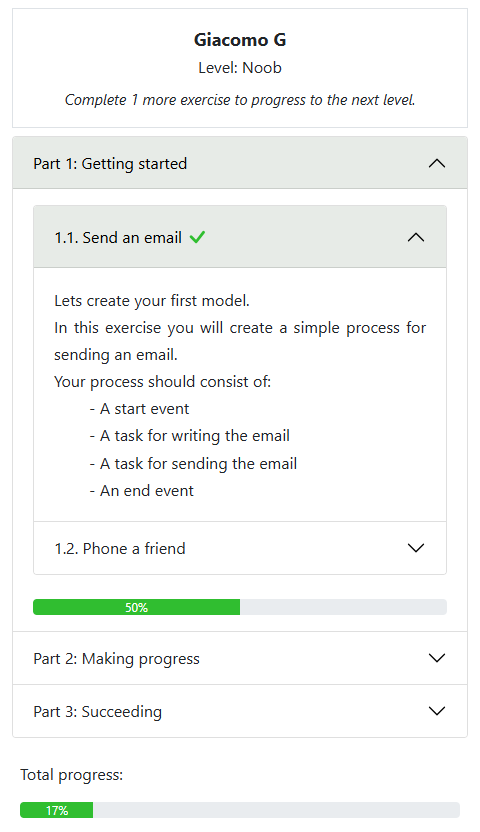
\includegraphics[width=0.4\linewidth]{Template_Latex_ScuDo_Tesi/Chapter3/progress_side.png}
    \caption{Application section showing the \textit{Progress} version}
    \label{fig:proto_progress}
\end{figure}

\begin{figure}[H]
    \centering
    \begin{subfigure}{0.48\linewidth}
        \centering
        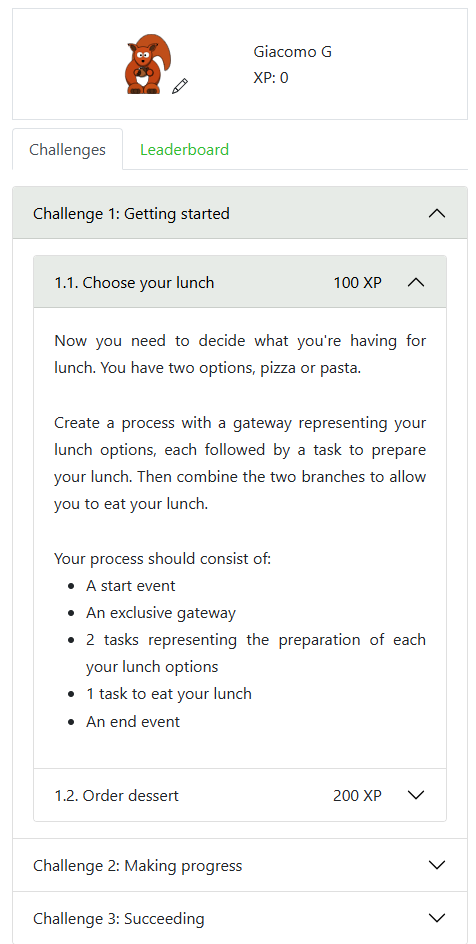
\includegraphics[width=\linewidth]{Template_Latex_ScuDo_Tesi/Chapter3/challenge_side1.png}
        \caption{Exercise text with the \textit{Competition} version's exclusive mechanic: obtainable experience points}
        \label{fig:proto_competition1}
    \end{subfigure}\hfill
    \begin{subfigure}{0.48\linewidth}
        \centering
        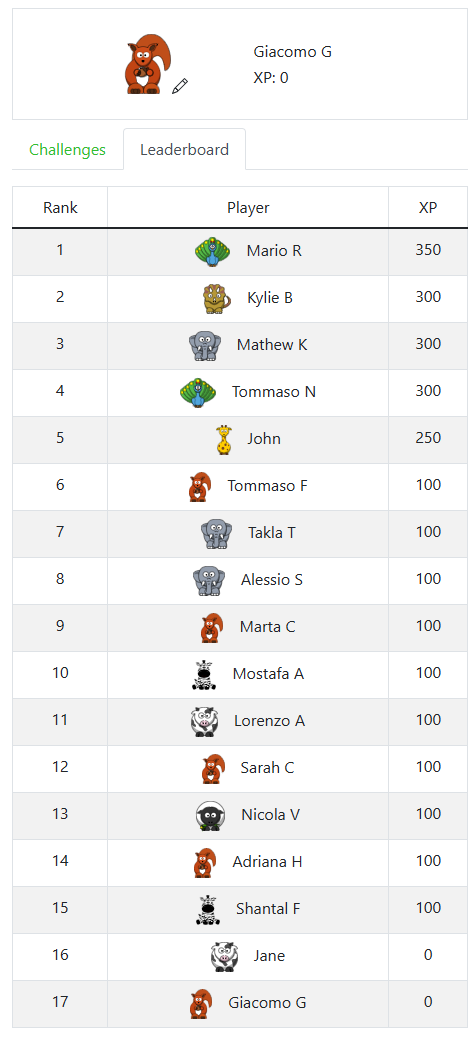
\includegraphics[width=\linewidth]{Template_Latex_ScuDo_Tesi/Chapter3/challenge_side2.png}
        \caption{Leaderboard shown in the \textit{Competition} version}
        \label{fig:proto_competition2}
    \end{subfigure}
    \caption{Application section showing the \textit{Competition} version}
    \label{fig:proto_competition}
\end{figure}

\begin{figure}[H]
    \centering
    \begin{subfigure}{0.48\linewidth}
        \centering
        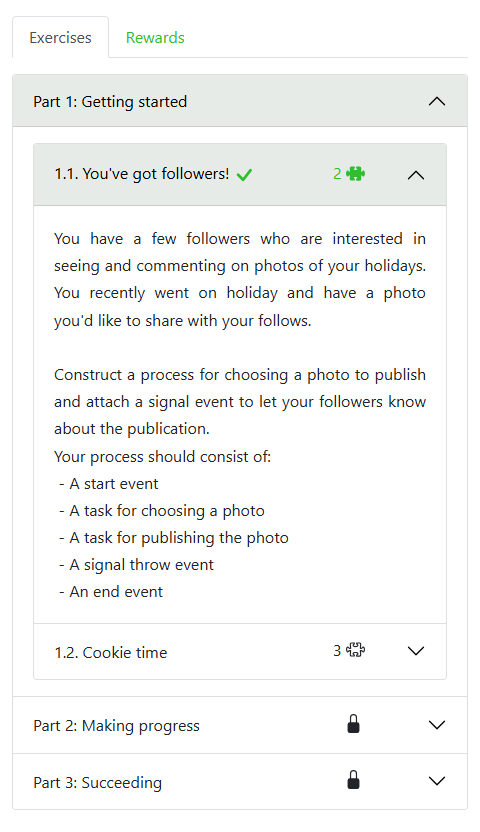
\includegraphics[width=\linewidth]{Template_Latex_ScuDo_Tesi/Chapter3/rewards_side1.png}
        \caption{Exercise text with the \textit{Rewards} version's exclusive mechanic: obtainable puzzle pieces and unlockable exercises}
        \label{fig:proto_rewards1}
    \end{subfigure}\hfill
    \begin{subfigure}{0.48\linewidth}
        \centering
        
\includegraphics[width=\linewidth]{Template_Latex_ScuDo_Tesi/Chapter3/rewards_side2.png}
        \caption{Completable puzzle shown in the \textit{Rewards} version}
        \label{fig:proto_rewards2}
    \end{subfigure}
    \caption{Application section showing the \textit{Rewards} version}
    \label{fig:proto_rewards}
\end{figure}

Following the definition of the three themes, and the subsequent identification of the associated game mechanics, the prototype was developed as a web application that offered three separate versions of the tool, each built around one theme. The underlying evaluation engine, the modeling environment adopted, the aesthetic layout of the application, and the feedback aspect were kept the same throughout the three versions, ensuring that any comparison between them would exclusively assess the impact of the different game mechanics, to identify the most effective ones in increasing motivation and interest.

Among the various options available for representing diagrams in an online canvas, \emph{bpmn.js} was selected, since it offered several benefits such as being easily integrable into web applications, the ability to create BPMN diagrams with ease thanks to drag-and-drop functionalities and easily editable elements, as well as offering developers easy access to the \emph{ElementRegistry}, a variable that contains all elements that are found in any given diagram, allowing easy access to the properties and information of the elements. The latter feature in particular was the one that let \emph{bpmn.js} stand out as the best option, as it allowed a way to define custom BPMN evaluation rules, leading to the creation of the dedicated evaluation engine. 

Another strong benefit of \emph{bpmn.js} consisted of it being an open-source project with an active online community where several extensions that enhance the modeling experience with additions such as providing graphical enhancements, simulating the process flow, allowing the insertion of custom elements, and identifying differences between two diagrams. Out of the several extensions available, the prototype was enhanced with one that offered linting capabilities: through a button added to the modeling environment, users would be able to have their diagram validated against BPMN modeling rules derived from good practices, and, if a diagram would contain errors, elements with errors would be enhanced with visual feedback. An example of how the feedback provided by the linter looks can be seen in Figure \ref{fig:linter}.

\begin{figure}[ht]
    \centering
    \frame{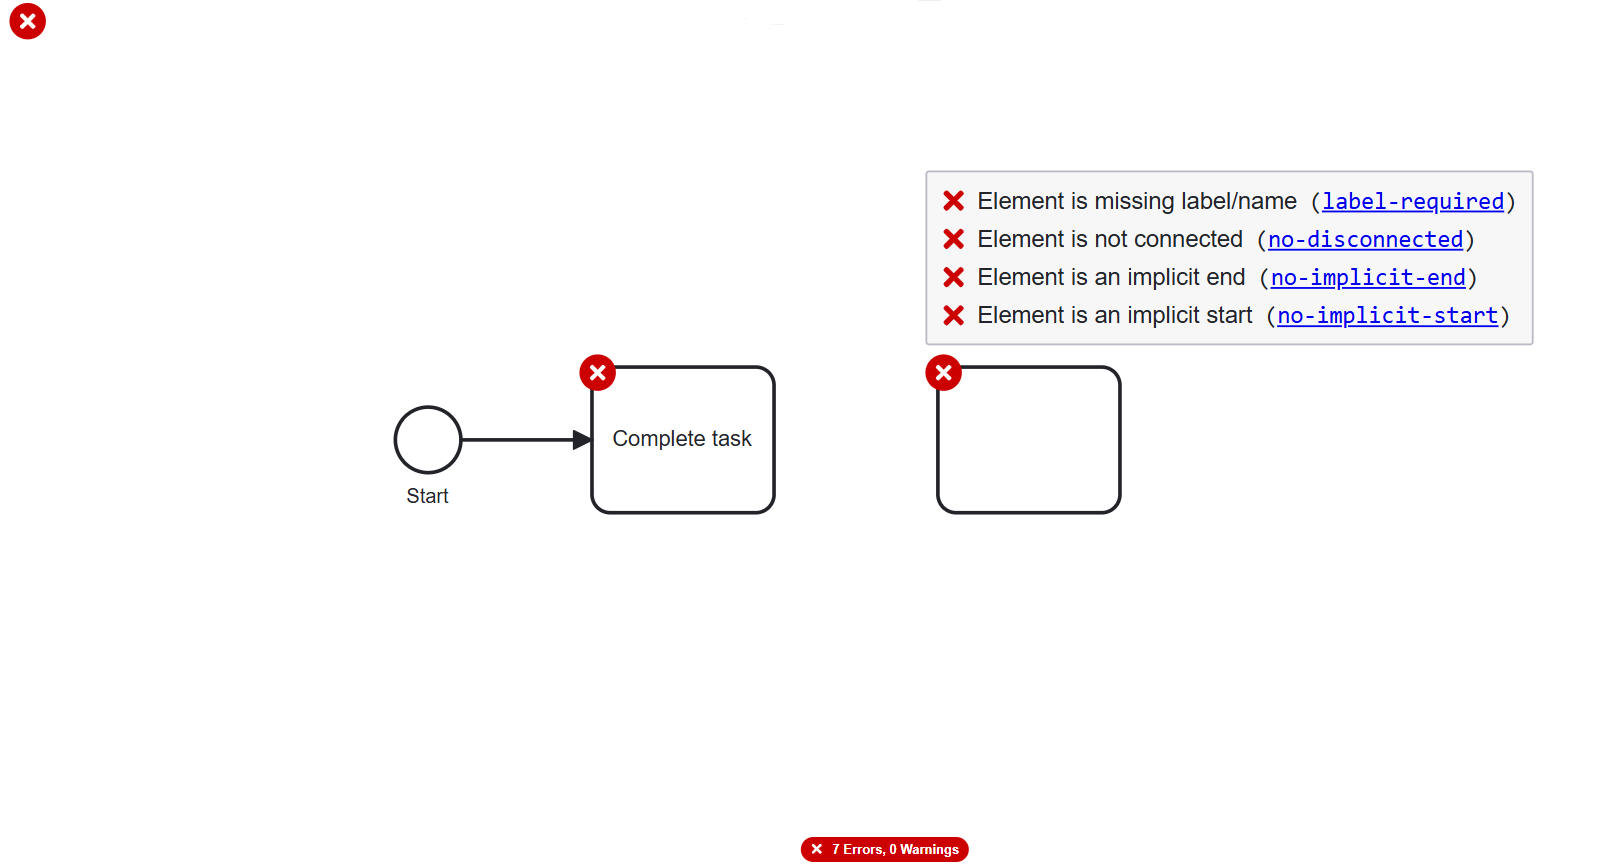
\includegraphics[width=1\linewidth]{Template_Latex_ScuDo_Tesi//Chapter3/bpmnlint.png}}
    \caption{BPMN linting extension highlighting elements with errors}
    \label{fig:linter}
\end{figure}

\subsection{Evaluation Engine}

A feature that was judged to be essential for the developed prototype is the implementation of an automated evaluation engine: by providing a way for students to submit their solution and receive automatic feedback the gamified tool would distinguish itself among the existing tools and approaches by allowing freedom in how students solve exercises, as the current educational options in the literature either offer static solution capabilities with element selection or are a real-life game where teacher feedback is required.

Furthermore, an automated feedback mechanism would solve the issue of BPMN education requiring practical assignments with teacher assistance, by easing the necessary workload and letting students receive preliminary assessments of their solutions, countering limited teacher availability and ensuring students are guided in a way that feels similar to what a human evaluator would do, with the teacher being available for complex assessments and corrections that the tool would not be able to catch.

The first step in the creation of this evaluation engine was achieved with the linting extension, which was selected due to it being able to identify violations to standard modeling constraints (e.g., processes requiring a single start event, elements not being disconnected from the main flow, execution flows needing to eventually reach an end event); the linter, however, would only be able to cover syntactic violations, while lacking a way to identify semantic ones (that is, it would not be able to understand whether a diagram is consistent with the domain it is supposed to represent).

For this purpose, six evaluation criteria have been defined for the prototype version of the tool, with the goal of identifying the first set of evaluation rules and conditions needed to have a valid automated evaluation procedure for BPMN diagrams; these first criteria were not exhaustive but would serve as the starting point for the creation of a complete engine. A specific section of the tool made it possible for a teacher to define evaluation conditions for an exercise by specifying the values related to each criterion by using the JavaScript Object Notation (JSON) format, using the element names defined by \emph{bpmn.js} to identify the required elements. (e.g., an activity would have to be specified as \emph{Task}, an exclusive gateway as \emph{ExclusiveGateway}).

The six criteria are as follows:
\begin{enumerate}
    \item Specific BPMN elements must be present in the diagram. This criterion is used to list the elements the student is expected to include in their diagram for it to be considered correct. Requires the teacher to state the type of element as key and the number of expected elements of that type as value:
    \begin{lstlisting}[language=json,firstnumber=1]
    {"StartEvent": 1, "Task": 2, "EndEvent": 1}
    \end{lstlisting}
    \item An element of a specific type must be followed by an element of a second type. This criterion allows teachers to define the expected order of elements in the diagram, letting them define the intended process flow. Works by specifying the target of preceding element as key and the destination element as value:
    \begin{lstlisting}[language=json,firstnumber=1]
    {"Target_ExclusiveGateway" : "Task"}
    \end{lstlisting}
    \item An element of a specific type must have a specific definition. Useful in case a solution requires events, this criterion lets teachers specify the intended cause of an event by using its type (start, intermediate, or end) as key and the definition as value:
    \begin{lstlisting}[language=json,firstnumber=1]
    {"Definition_IntermediateCatchEvent" : "TimerEventDefinition"}
    \end{lstlisting}
    \item An element of a given pool must send a message flow to one in a different pool. If communication between different pools must be represented, this criteria lets teachers specify which element is sending the message as key, and which element is receiving the message as value:
    \begin{lstlisting}[language=json,firstnumber=1]
    {"MessageFlow_Task" : "StartEvent"}
    \end{lstlisting}
    \item A gateway must have a given number of outgoing sequence flow. With this criterion, decision splits can be modeled by stating how many flows are supposed to go out of a gateway by specifying the type of gateway as key and the number of flows as value:
    \begin{lstlisting}[language=json,firstnumber=1]
    {"Outgoing_ExclusiveGateway" : 2}
    \end{lstlisting}
    \item A gateway must have a given number of incoming sequence flow. The final criterion mirrors the previous one by stating how many incoming flows are expected for gateways, with the two criteria being intended to be used in the same fashion if a solution includes gateways by specifying a pair of two (key, value) items for each gateway. The definition of data needed for this criterion is similar to that of the fifth one:
    \begin{lstlisting}[language=json,firstnumber=1]
    {"Incoming_ExclusiveGateway" : 2}
    \end{lstlisting}
\end{enumerate}

The automated evaluation engine works by retrieving the full set of rules specified according to the six criteria and, any time a student asks for an automated evaluation, iterates through the elements in the diagram to check if there are elements that satisfy the specified condition. A rule is satisfied if there is one element in the diagram that satisfies its corresponding condition, and this check applies to rules defined according to all criteria excluding the first one; rules defined according to the first criteria simply verify the number of elements of each given type, without any check on their properties.

The evaluation engine built for the prototype offers a basic automated grading system, not intended to act as a complete example of automated BPMN evaluation but instead serving as a guide that provides clarity on which elements are required for a diagram. Unfortunately, the implementation of the engine has a serious limitation: the fact that checks are based on the existence of nodes with no assessment of their name or position in the flow means that, for example, given two tasks that are supposed to be one after the other in the intended solution and have their positions swapped in a student's solution, the system would consider them correct anyway, because the rule simply states that two tasks must exist and that one must be followed by another.

This limitation meant that, at least in the first prototype version, the tool was not able to identify semantic violations, but would only be usable as a way for students to learn good modeling practices; these six criteria were meant to be a starting point to assess the impact of gamification mechanics for the solution of BPMN exercises: once the best mechanics would have been identified, an improved evaluation engine would have been created to support an improved version of the tool.

\subsection{Preliminary prototype assessment}

Once the first prototype had been successfully developed, and its name had been finalized as \textbf{BIPMIN}, a preliminary assessment in the form of a single trial was performed to evaluate both the usability of the tool and the effectiveness of the three different versions, with the corresponding game mechanics, in increasing student motivation. The purpose of the study was defined according to the Goal-Question-Metric (GQM) template and was expressed as \emph{evaluate and improve the usability and motivation of participants in using different game elements in motivating students to interact with a gamified BPMN modeling application from the point of view of software development researchers in the context of an educational environment}; Table \ref{tab:gqm3_proto} summarizes the study's purpose according to the GQM template.

\begin{table}[ht]
\small
\centering
\caption{GQM Template for the preliminary assessment of BIPMIN}
\begin{tabular}{@{}p{0.3\columnwidth} p{0.55\columnwidth}@{}}
\toprule
Object of Study & Gamified BPMN modeling application prototype\\ 
Purpose & Evaluate and improve \\
Focus & Effectiveness at encouraging student interest \\
Context & University SE courses \\
Perspective & Developers, researchers, teachers \\ \bottomrule
\end{tabular}
\label{tab:gqm3_proto}
\end{table}

\subsubsection{Study Design and Participants}

The preliminary trial was set up as a session where participants would have to complete a predefined number of tasks to evaluate the BIPMIN prototype. The first task consisted of getting familiar with the BPMN modeling environment implemented in the tool by solving a first assignment on the online platform \emph{bpmn.io}; this first task aimed at giving participants a baseline reference of how non-gamified BPMN modeling is performed, which would then be compared with the enhanced aspects brought by gamification. After completing the second task (successfully accessing the application via login), participants were asked to perform three tasks, consisting of completing one BPMN modeling exercise for each task; following successful completion of these three tasks, participants were asked to perform an additional exercise with the version they had found more interesting. The final task was optional, and consisted of participants solving further exercises with their preferred version if they wished to do so. Completion of two post-trial surveys was needed to complete the study. A summary of all seven tasks performed during the trial is presented in Table \ref{tab:tasks}.


\begin{table}[H] 
\centering
\footnotesize
\caption{List of tasks that composed the pilot trial} 
\begin{tabular}{cp{0.895\textwidth}} 
\toprule
 \textbf{Task} & \textbf{Description}\\ 
\midrule
\textbf{T1} & Complete the tutorial, then ask the facilitator to check your solution when you are done \\ 
\midrule
\textbf{T2} & Access your account using the credentials provided. \\ 
\midrule
\textbf{T3} & 1. Select the progress version and complete the first exercise. \\
   & 2. Check the skill level you reached after completing one exercise. \\
   & 3. Return to the homepage. \\ 
\midrule
\textbf{T4} & 1. Select the competition version and complete the first exercise. \\ 
   & 2. Check the position you reached on the leaderboard. \\ 
   & 3. Choose your avatar. \\ 
   & 4. Return to the homepage. \\ 
\midrule
\textbf{T5} & 1. Select the rewards version and complete the first exercise. \\ 
   & 2. Check how many puzzle pieces you have unlocked. \\ 
   & 3. Return to the homepage. \\ 
\midrule
\textbf{T6} & Complete 1 additional exercise from the version you prefer. \\ 
\midrule
\textbf{T7} & If you wish, complete further exercises with the version you prefer, then fill out the post-experiment survey. \\ 
\bottomrule
\end{tabular}
\label{tab:tasks}
\end{table}

The trial was performed in person at Politecnico di Torino for 10 participants, who used a version of the prototype running locally on a laptop and answered to paper copies of the questionnaire; the two remaining participants could only take part in the study remotely, and thus used remote desktop control to access the local prototype.

Participants were selected via convenience sampling among students of the Masters' degree in Computer Engineering at Politecnico di Torino as representative of students that would learn BPMN during their study career; due to the trial being a preliminary study, a small number of participants was selected, with a total of 12 volunteering students being involved. Participation in the study was rewarded with tangible prizes such as free snacks offered by the thesis student who was overseeing the development of the prototype, Ms. Kylie Bedwell. 

Since the trial consisted of comparing three different implementations of the BIPMIN prototype, the study design needed to ensure that participants could try all three versions to conduct fair judgment; it was thus not possible to adopt a between-subjects technique where each participant would try only one of the three versions of the prototype and there would be no way to compare the differences in game mechanics. For this purpose, a within-subjects design (see Section \ref{sec:empirical_methods}) was selected, so that participants could experience all three versions of the prototype for direct comparison; the design is also more suited for experiments with a small sample of participants, making it the better choice for the pilot study. To mitigate ordering biases, tasks were counter-balanced with the use of a balanced Latin square to ensure participants did not test the prototype with the same configuration; this resulted in a total of 6 different variations of how tasks T3, T4, and T5 were ordered, each assigned to two of the participants, as shown in Table \ref{tab:latinsquare}.

\begin{table}[H] 
\centering
\small
\caption{Task order based on a balanced Latin~square.} 
\setlength{\tabcolsep}{12.2mm}
\begin{tabular}{ccc} \toprule
\textbf{First} & \textbf{Second}& \textbf{Third}\\ \midrule
T3 & T4 & T5 \\
T4 & T5 & T3 \\
T5 & T3 & T4 \\
T3 & T5 & T4 \\
T4 & T3 & T5 \\
T5 & T4 & T3 \\ \bottomrule
\end{tabular}
\label{tab:latinsquare}
\end{table}

Finally, the exercises that were used for the trial were the same across the different versions, with the only difference being in the order in which they were supplied depending on the version used: for example, the first exercise to appear in the rewards version was used as the fourth one in the competition version; the exercises had a similar level of difficulty, ensuring that the level of challenge would remain the same over the different tasks, as well as making sure that participants were able to face different exercises and modeling topics throughout the study.

\subsubsection{Research Questions and Metrics}

Three research questions have been defined to frame the design of the preliminary assignment:
\begin{itemize}
    \item \textbf{RQ1: } Is the system effective in motivating students to perform modeling tasks? \\
        \emph{The expectation is that, by using BIPMIN, participants are able to successfully complete modeling assignments and are more encouraged in doing them}
    \item \textbf{RQ2: } What is the usability of the system?\\
        \emph{The goal of this question is to measure the usability of the prototype and identify potential improvement areas}
    \item \textbf{RQ3: } Which game elements are preferred by the users of the system?\\
        \emph{The goal of this question is to identify the elements that participants identify as the most motivating and enjoyable, to build upon them for a complete version of the tool suitable for classroom use}
\end{itemize}

To answer RQ1, the goal was to assess whether the prototype could help the participants by improving their performance in BPMN modeling tasks, as well as to evaluate whether the implemented mechanics could be effective in increasing the motivation to perform additional tasks. For this purpose, the tasks that composed the trial were defined to ensure that the participants to the study could:

\begin{itemize}
    \item Successfully access the application
    \item Navigate to their target location
    \item Understand how to perform and complete exercises within the application
    \item Understand the feedback provided by the application to fix any errors
    \item Interact positively with the different game elements
\end{itemize}

Additionally, quantitative measures were taken as a way to assess the impact, in terms of performance and motivation, of the BIPMIN tool: for all tasks and sub-tasks, excluding the optional task T7, the time needed was considered a relevant metric, with a reference value being defined as the reference time needed to complete the task (e.g., the time needed for successfully completing an exercise was estimated as 5 minutes, a time considered reasonable according to the difficulty of the various exercises). Another metric, for tasks related to completing exercises, was the number of times participants checked the solutions of their exercises; this metric was recorded to measure whether participants would understand the feedback mechanism of the tool. The summary of the tasks, with the corresponding criterion that was considered necessary for successful completion and reference time needed to achieve the criterion, is presented in Table \ref{tab:successCriteria}.

\begin{table}[ht] 
\centering
\footnotesize
\caption{RQ1-related success criteria and metrics for the tasks}
\begin{tabular}{cp{0.5\textwidth}p{0.365\textwidth}} \toprule
 \textbf{Task} & \textbf{Success Criteria} & \textbf{Metrics} \\ \midrule
T1 & The participant follows the instructions provided and is able to complete the exercise (in 5 min) & Time to complete \\
& & Number of requests to check the solution \\ 
\midrule
T2 & The participant logs in to the tool successfully (in 30 s) & Time to complete \\ 
\midrule
T3 & 1. The participant completes the first exercise (in 5 min) & Time to complete \\ 
& 2. The participant records their level (in 30 s) & Number of clicks on the check solution button \\ 
& 3. The participant returns to the home screen (in 30 s) & \\ 
\midrule
T4 & 1. The participant completes the first exercise (in 5 min) & Time to complete \\ 
& 2. The participant records their rank (in 30 s) & Number of clicks on the check solution button \\ 
& 3. The participant selects a new avatar (in 2 min) & \\ 
& 4. The participant returns to the home screen (in 30 s) &  \\ 
\midrule
T5 & 1. The participant completes the first exercise (in 5 min) & Time to complete \\ 
& 2. The participant records the number of pieces collected (in 1 min) & Number of clicks on the check solution button \\ 
& 3. The participant returns to the home screen (in 30 s)  & \\ 
\midrule
T6 & The participant completes an additional exercise on their preferred version (in 5 min) & Time to complete \\ 
& & Number of clicks on the check solution button \\ 
\midrule
T7 & N/A & \\ \bottomrule
\end{tabular} 
\label{tab:successCriteria}
\end{table}


To answer RQ2, which focused on assessing the usability of the BIPMIN prototype, the System Usability Scale described in Section \ref{sec:empirical_methods} \cite{brooke1996sus} was used, leading to the computation of the final score intended to measure the perceived usability of the BIPMIN prototype.

To answer RQ3, the three versions of the prototype were developed according to the themes discussed back in Section \ref{sec:proto_tool}, with the corresponding metrics being implemented, keeping the visual aesthetic of the application and the feedback mechanism the same over all three versions.

During the trial, multiple metrics were considered in relation to RQ3: the first one concerned participant behavior in terms of choosing their preferred version for task T6, which asked them to complete an additional fourth exercise after having tried the three versions once, clearly highlighting the preferred game elements. The optional task T7 was included to further reinforce the preference, to assess whether which of the implemented game elements were considered motivating and appealing enough to have students perform more exercises than what they were asked to.

Additional metrics were recorded through a post-study survey that aimed to record the participants' preference composed of seven questions. More precisely, the survey included: one question asking participants to select which versions of the prototype they would like to use if they were to keep learning BPMN; two questions where participants had to rank the three versions according to how motivating and enjoyable they felt, with a score of 3 indicating the most motivating/enjoyable version, and a score of 1 the least; two questions asking participants to rank the eight game elements according to how motivating and enjoyable they felt, with increasing scores from 1 to 8; a question where participants had to specify which game elements they recommended including in a complete version of BIPMIN. The questionnaire was then concluded with a section for open comments to gather feedback and participant responses. Through the inclusion of this survey it was possible to have a clear understanding of the relative perception of each mechanic in terms of increasing motivation, to then focus on the most appreciated mechanics for further development of the prototype and actual classroom use. 


\subsubsection{Results}

To answer RQ1, two metrics were taken: the time needed by the participants to complete all tasks, and the number of times each participant evaluated their solution during the tasks associated with modeling exercises. Regarding the time metric, Table \ref{tab:time} lists, for each participant, the time spent for each task and the overall average time among all participants; time measures are considered in relation to the success criteria defined back in Table \ref{tab:successCriteria}, with students being considered successful if their time score was less than the expected time for each task. A special mention regarding task timing needs to be given for tasks T3.3, T4.4, and T5.3, the three tasks that happened when a participant had successfully completed an exercise and had to return to the homepage. This activity could be completed by clicking on the application logo in the upper sidebar of the screen, and the corresponding tasks were repeated three times in different order, meaning that participants would get familiar with how to complete the task in the second and third exercise, and would thus need around 1-2 seconds to return home. The three tasks have been considered equivalent, in the sense that the time needed to complete the first of these tasks has been considered for computing the average time.

\begin{table}[h]
\centering
\footnotesize
\caption{Task completion times. Times that exceeded the expected duration are shown in bold.}
\resizebox{\textwidth}{!}{%
\begin{tabular}{lcccccccccccc}
\hline
\textbf{Participant} & \textbf{T1} & \textbf{T2} & \textbf{T3.1} & \textbf{T3.2} & \textbf{T4.1} & \textbf{T4.2} & \textbf{T4.3} & \textbf{T5.1} & \textbf{T5.2} & \textbf{T6} & \textbf{T7} & \textbf{T3.3/T4.4/T5.3} \\
\hline
P1  & 3:45 & 00:16 & 1:22 & 00:02 & 4:50 & 00:06 & 00:10 & \textbf{5:46} & 00:10 & 4:12 & Y & 00:12 \\
P2  & 4:14 & 00:10 & 2:22 & 00:04 & 3:45 & 00:05 & 00:04 & \textbf{7:01} & 00:06 & \textbf{5:50} &  & 00:03 \\
P3  & 2:57 & 00:08 & 2:53 & 00:05 & 4:31 & 00:16 & 00:04 & 4:00 & 00:02 & 3:10 & Y & 00:05 \\
P4  & 3:47 & 00:08 & 1:48 & 00:18 & 3:41 & 00:02 & 00:05 & 4:49 & 00:12 & 4:21 &  & 00:07 \\
P5  & 4:02 & 00:05 & 2:58 & 00:02 & 4:10 & 00:03 & 00:04 & \textbf{6:34} & 00:09 & 3:03 &  & 00:02 \\
P6  & 2:52 & 00:10 & 1:03 & 00:15 & 3:15 & 00:10 & 00:09 & 4:45 & 00:02 & 3:47 & Y & 00:12 \\
P7  & 2:22 & 00:10 & \textbf{5:56} & 00:02 & 3:58 & 00:03 & 00:02 & 3:02 & 00:02 & \textbf{6:11} &  & 00:14 \\
P8  & N/A  & 00:10 & 3:32 & 00:02 & \textbf{8:53} & 00:15 & 00:04 & \textbf{5:05} & 00:02 & \textbf{6:46} &  & 00:12 \\
P9  & N/A  & N/A  & 4:57 & 00:02 & \textbf{7:50} & 00:01 & 00:03 & \textbf{9:31} & 00:12 & \textbf{9:09} &  & 00:30 \\
P10 & 3:13 & 00:28 & 1:51 & 00:22 & 4:03 & 00:14 & 00:08 & 1:56 & 00:03 & 3:55 &  & \textbf{00:36} \\
P11 & 3:29 & 00:30 & 2:23 & 00:08 & 1:26 & 00:08 & 00:06 & 2:48 & 00:03 & 2:23 &  & 00:06 \\
P12 & 4:49 & 00:21 & 2:59 & 00:06 & 4:09 & 00:09 & 00:13 & 4:25 & 00:03 & \textbf{5:21} &  & 00:25 \\
\hline
Average & 3:33 & 00:14 & 2:50 & 00:07 & 4:32 & 00:07 & 00:06 & 4:58 & 00:05 & 4:50 & N/A & 00:13 \\
\hline
\end{tabular}
}
\label{tab:time}
\end{table}


By observing the resulting set of collected times, it can be seen that the time needed by participants to complete each task is, on average, below the corresponding success criteria for the task, implying that participants were able to successfully use BIPMIN for its intended purpose of being an engaging modeling environment. 

Going more into detail, there were 13 instances of participants taking more than the expected 5 minutes to complete a modeling exercise, and six of these happened to the participants who were performing the trial remotely, with interaction lag being caused by the remote control, implying that the corresponding scores could have been lower and more in line with the scores obtained by the in-person participants (although still above the expected threshold) if the task had been performed live.

By observing the overall distribution of tasks requiring more time than expected, most of them happened in task T5.1, the one associated to the \textit{Rewards} theme: the fact that the order of execution was different, as well as the order in which exercises are faced, suggests that this version of the prototype could possibly be perceived as more interesting, as participants would spend more time exploring it compared to the other two while also completing exercises.

Finally, 5 participants out of 13 did not manage to complete task T6 in less than 5 minutes; this result is in line with the overall design of the study, as the exercises were designed to have a growing difficulty level, with the fourth exercise being slightly more complex than the preceding three, and thus requiring more time than the others.

The second metric that was collected for RQ1 consisted of the number of times participants checked their solution with the automated evaluation engine when performing a task associated with a modeling exercise. Through this metric, the goal was to assess the effectiveness in the feedback mechanism in helping users fix errors present in their diagrams, and, with feedback being a common mechanic and successful completion being necessary for satisfying each of the three versions' game mechanics, assess whether BIPMIN could be effective in motivating students. The count of checks for each participant in the four modeling tasks, as well as for the tutorial task T1 performed outside BIPMIN, can be viewed in Table \ref{tab:checks}.

\begin{table}[H]
\centering
\small
\caption{Number of automated evaluation checks performed during exercise-related tasks.} 
\setlength{\tabcolsep}{8.7mm}
\begin{tabular}{lccccc} \toprule
\textbf{Participant}& \textbf{T1} & \textbf{T3.1} & \textbf{T4.1} & \textbf{T5.1} & \textbf{T6}\\ 
\midrule
P1 & 2 & 1 & 3 & 4 & 3 \\
P2 & 1 & 5 & 3 & 1 & 3 \\
P3 & 1 & 2 & 3 & 2 & 1 \\
P4 & 1 & 3 & 3 & 3 & 1 \\
P5 & 1 & 3 & 2 & 2 & 2 \\
P6 & 2 & 1 & 2 & 2 & 1 \\
P7 & 1 & 3 & 1 & 1 & 2 \\
P8 & 1 & 2 & 2 & 2 & 2 \\
P9 & 1 & 1 & 2 & 1 & 1 \\
P10 &1 & 2 & 2 & 1 & 1 \\
P11 &1 & 1 & 2 & 2 & 2 \\
P12 &1 & 4 & 2 & 2 & 6 \\ 
\bottomrule
\end{tabular}
\label{tab:checks}
\end{table}

It can be observed that most participants needed a low number of checks before reaching a correct solution, implying that the feedback mechanism was effective in guiding them towards successful exercise completion; furthermore, the cases where participants needed 4 or more checks before completing an exercise happened when performing later tasks such as the third in their planned order, or during T6, meaning that these values were obtained when performing more complex exercises. The fact that the number of necessary checks was still somewhat low even for the more complex exercises highlights the effectiveness of the evaluation engine's feedback mechanism and the game mechanics associated with the results of an evaluation.

\answer{RQ1}{The average time needed to complete modeling tasks being below the expected necessary time implies that applying gamification had no negative impact in successful BPMN modeling, and could actually be seen as a motivating factor. The implementation of a feedback mechanism and of game mechanics being tied to exercise completion, tied with the on average low number of checks needed to complete exercises further reinforces this assumption, as gamification could be seen as having a strong impact on guiding students to the creation of correct solutions.}

To answer RQ2, the System Usability Scale (SUS) was given to the participants to fill at the end of the study, to measure its perceived usability by students and assess whether it would be appreciated if it were to be used in a classroom environment. After computing the score with the answers given by all participants (a summary of which can be found in Table \ref{tab:sus}), the final SUS score obtained by the BIPMIN prototype was computed as the average of the scores given by all participant, resulting in a total score of 85.8. The resulting score is above 68, the score canonically considered to be the average usability score of software applications, implying good usability characteristics and a user-friendly design for the prototype. However, the low number of participants is not sufficient to draw a conclusion in terms of the actual usability level of the application.

%This number indicates that the BIPMIN application exhibits good usability characteristics, being more than above the average computed by Sauro \cite{sauro2011practical}, the most extensive study on the SUS survey, which ranks five hundred different evaluations made with the scale. To add more perspective, a study by Pekpazar et al. \cite{Pekpazar} ranked four of the most commonly used mobile applications by a sample of 222 participants (YouTube, Facebook, WhatsApp, Mail app) with the SUS survey: results show an average score, respectively, of 84.02, 73.19, 87.32 and 76.72. The score obtained by the BIPMIN tool is comparable to the ones obtained by the four applications, but the small sample of participants must be considered: a large-scale experiment with more participants is almost certain to yield a different score, which may be in line with the one obtained in this study.


\begin{table}[ht]
    \centering
    \caption{System Usability Scale (SUS) scores given by the participants}
    \begin{tabular}{lccccccccccc}
    \toprule
    \textbf{Participant} & \textbf{Q1} & \textbf{Q2} & \textbf{Q3} & \textbf{Q4} & \textbf{Q5} & \textbf{Q6} & \textbf{Q7} & \textbf{Q8} & \textbf{Q9} & \textbf{Q10} & \textbf{Score}\\
    \midrule
         P1 & 4 & 2 & 5 & 1 & 5 & 1 & 4 & 1 & 5 & 2 & 90 \\
         P2 & 4 & 2 & 3 & 2 & 4 & 1 & 4 & 2 & 4 & 4 & 70 \\
         P3 & 5 & 1 & 4 & 1 & 5 & 1 & 5 & 1 & 5 & 2 & 90 \\
         P4 & 5 & 5 & 5 & 1 & 5 & 1 & 5 & 1 & 4 & 1 & 97.5\\
         P5 & 4 & 3 & 3 & 3 & 4 & 1 & 4 & 3 & 3 & 2 & 65 \\
         P6 & 4 & 1 & 5 & 1 & 5 & 1 & 5 & 1 & 5 & 3 & 92.5\\
         P7 & 5 & 1 & 5 & 2 & 5 & 1 & 3 & 2 & 5 & 1 & 90 \\
         P8 & 4 & 1 & 4 & 2 & 5 & 1 & 5 & 2 & 4 & 2 & 85 \\
         P9 & 4 & 1 & 4 & 1 & 4 & 1 & 3 & 2 & 4 & 2 & 80 \\
         P10& 5 & 1 & 5 & 1 & 5 & 1 & 5 & 1 & 5 & 2 & 97.5\\
         P11& 5 & 1 & 4 & 1 & 5 & 1 & 5 & 2 & 4 & 1 & 92.5\\
         P12& 4 & 1 & 4 & 2 & 5 & 1 & 4 & 1 & 3 & 3 & 80 \\
    \bottomrule
    \end{tabular}
    \label{tab:sus}
\end{table}

In addition to the SUS score, positive comments by the participants when using the tool were also noted and highlighted key points such as the pleasant application design, its ease of use and intuitive functionalities, as well as the intention to continue using the application for BPMN modeling. While the high SUS score and favorable opinions imply that BIPMIN could be easily understood and used by students during courses, the fact that there is no indication of how usability translate to increased efficiency must be considered, as well as the fact that with the SUS survey it is not possible to identify potential improvement areas in the tool design.

\answer{RQ2}{The BIPMIN prototype obtained a System Usability Score rating of 85.8, which is more than the average usability value for software applications; the score, together with the positive comments given by the participants when using the application, implies that the tool could be used in classroom environments and easily understood and appreciated. However, a high usability value may not necessarily imply effectiveness for improving BPMN modeling knowledge, meaning that additional work may be required.}

To answer RQ3, measures were taken to record the participants' preferences in terms of which version they liked the most, as well as their preferences on the game mechanics, observing not only which ones the participants liked the most, but which ones they had found motivating and enjoyable as well. The first step to observe these preferences was achieved with the inclusion of tasks T6 and T7: the first one explicitly asked participants to complete an additional exercise on their preferred version, while the latter was optional and asked participants to perform further exercises, using multiple versions if they wished. 

Participants showed a clear preference towards the \textit{Rewards} version, which was selected by 8 out of the 12 participants for task T6, while the remaining two versions were picked by two participants each; regarding T7, only three participants opted to solve more exercises, with one participant continuing to work on the \textit{Rewards} version, one continuing to use the \textit{Progress} version, and one moving from the \textit{Competition} version to the \textit{Rewards} one. The high appreciation for the \textit{Rewards} version can probably be attributed to how it ties successful modeling to receiving tangible, in-game, rewards: the fact that exercises have to be unlocked gives a sense of fulfillment when solving harder exercises, and the element of mystery represented by the hidden puzzle also encourages participants to choose said version over one that focuses on a single-use leaderboard or that indicates progression with no changes but the title.

Furthermore, the post-study survey aimed at exploring the participants' preferences more in detail; the first question focused on asking participants to mark which of the three versions they would use if they were to keep studying BPMN in the future, allowing for multiple versions to be selected. The selections have been combined to identify the relative level of preference between the three versions; the total count of answers to the first question can be seen in Figure \ref{fig:proto_rq3_pref_versions}.

\begin{figure}[H]
    \centering
    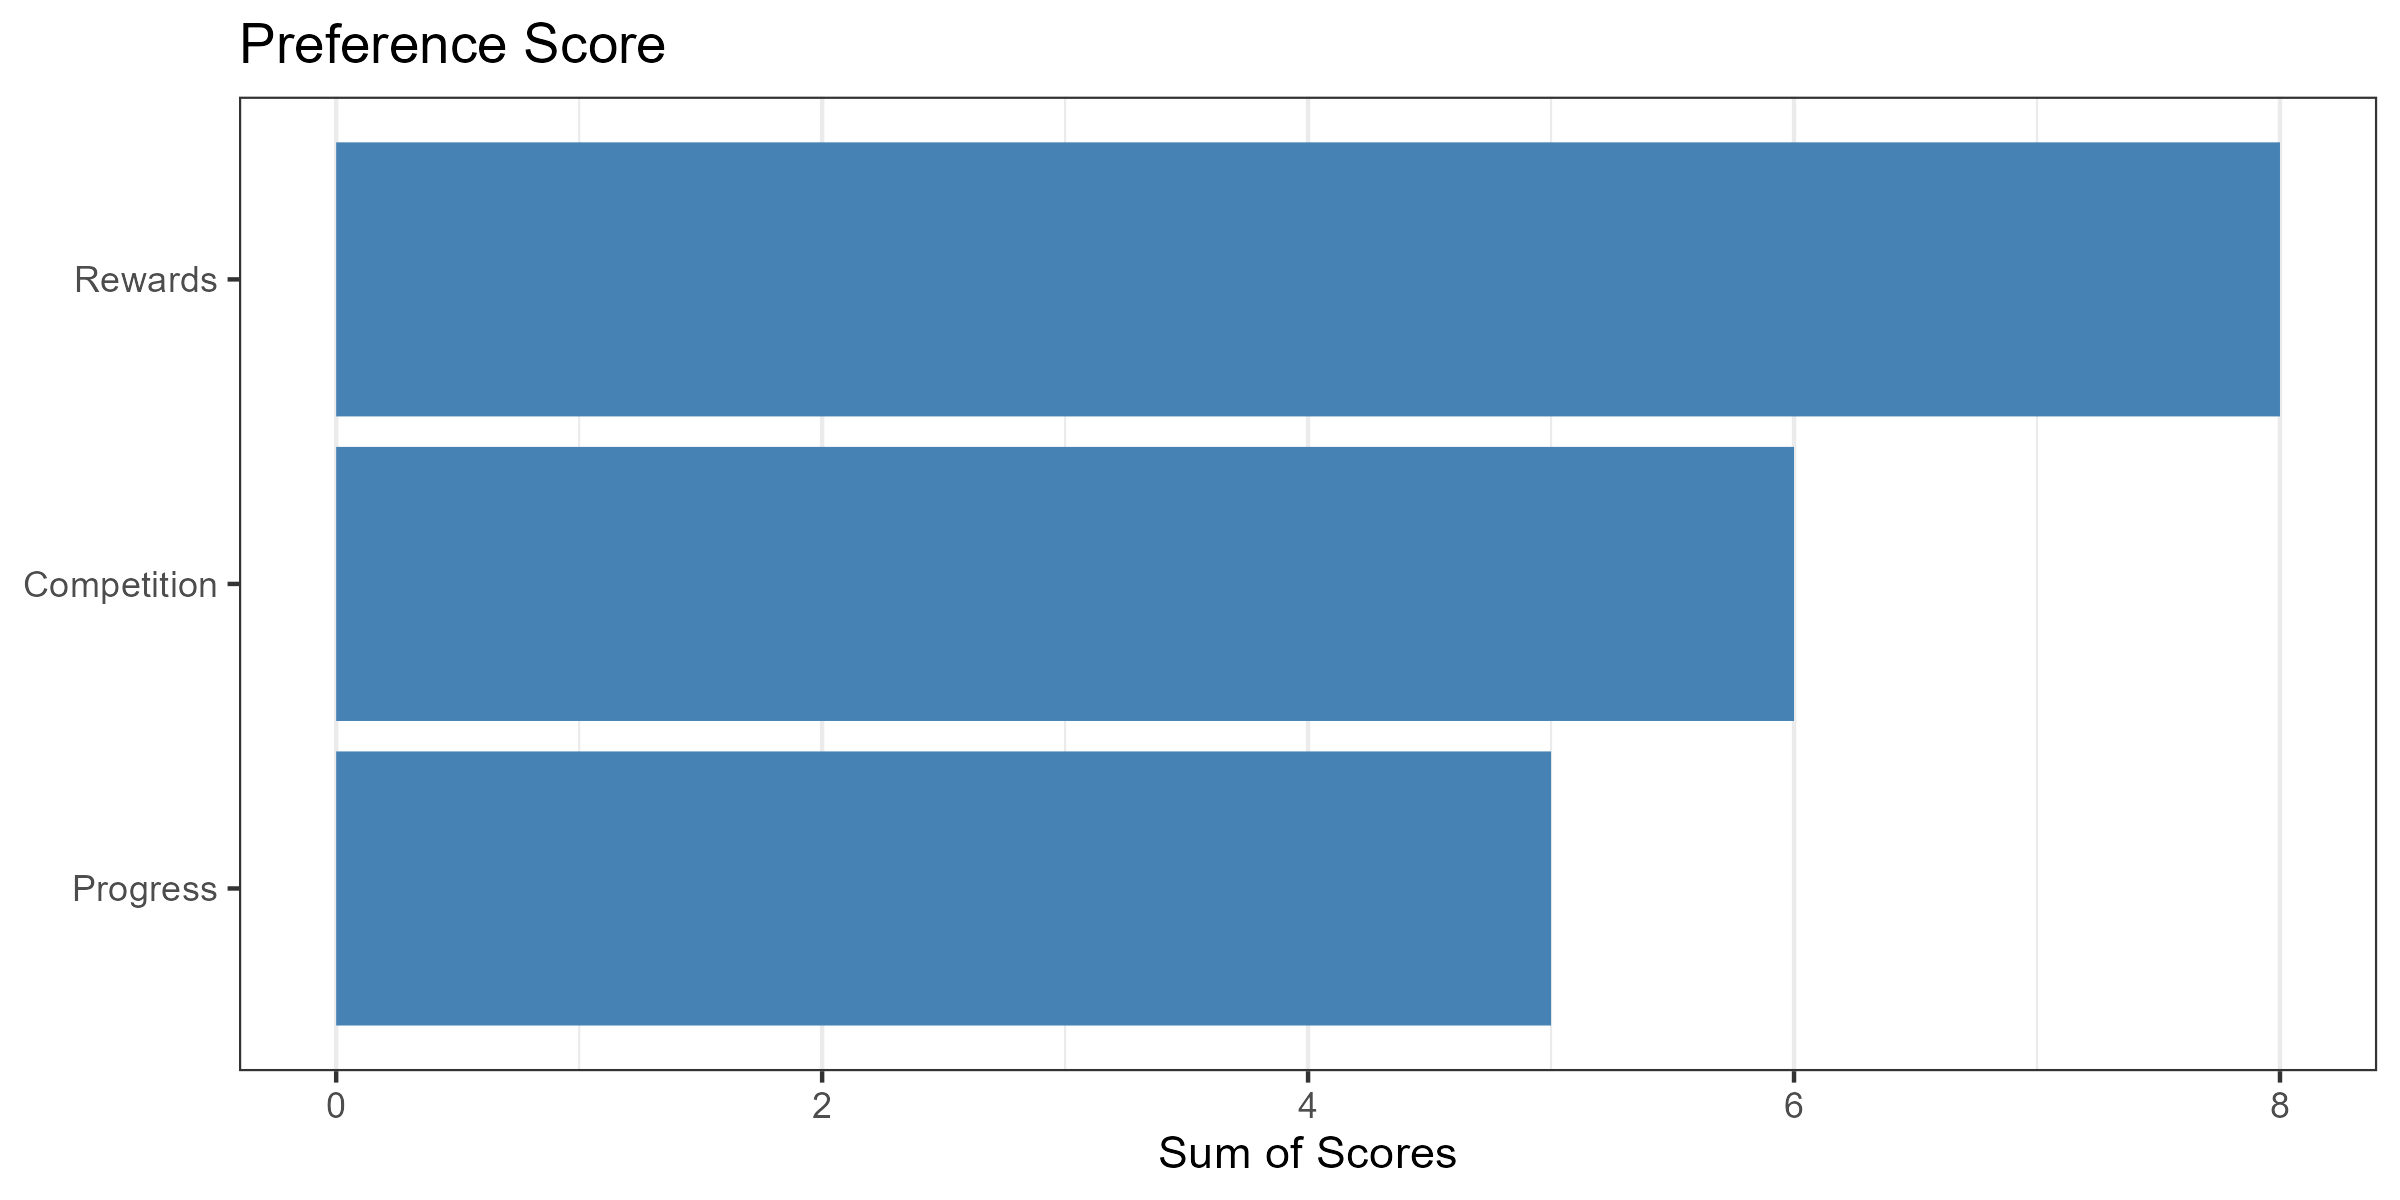
\includegraphics[width=1\linewidth]{Template_Latex_ScuDo_Tesi//Chapter3/proto_rq3_pref_versions.png}
    \caption{Count of the preferences expressed by participants about which versions they would be more likely to use}
    \label{fig:proto_rq3_pref_versions}
\end{figure}

Here as well, the \textit{Rewards} version appears as the most appreciated, with 8 participants stating they would like to use it again; the \textit{Competition} version was also fairly appreciated, with half of the participants selecting it, while the \textit{Progress} version was appreciated slightly less, gaining only 5 positive answers. This distribution further reinforces the hypothesis that unlockable elements are more appreciated, at least for a single session, and that users tend to prefer having tangible rewards tied to their progression rather than just visual feedback such as a growing progress bar.

To further explore the preferences related to the three versions, the survey also asked participants to rank the three game versions according to how motivating and enjoyable they found them, giving scores from 1 to 3; in two cases, two participants assigned the same score to two versions, leading to the score being split evenly to ensure a valid distribution of preference. The total scores for each version have been added together to compute the \textit{Enjoyment Score} and \emph{Motivation Score} for the three versions, and the distribution of these scores can be seen in Figure \ref{fig:proto_rq3_enj_versions} and \ref{fig:proto_rq3_motiv_versions}, respectively.

\begin{figure}[H]
    \centering
    \begin{subfigure}{0.9\linewidth}
        \centering
        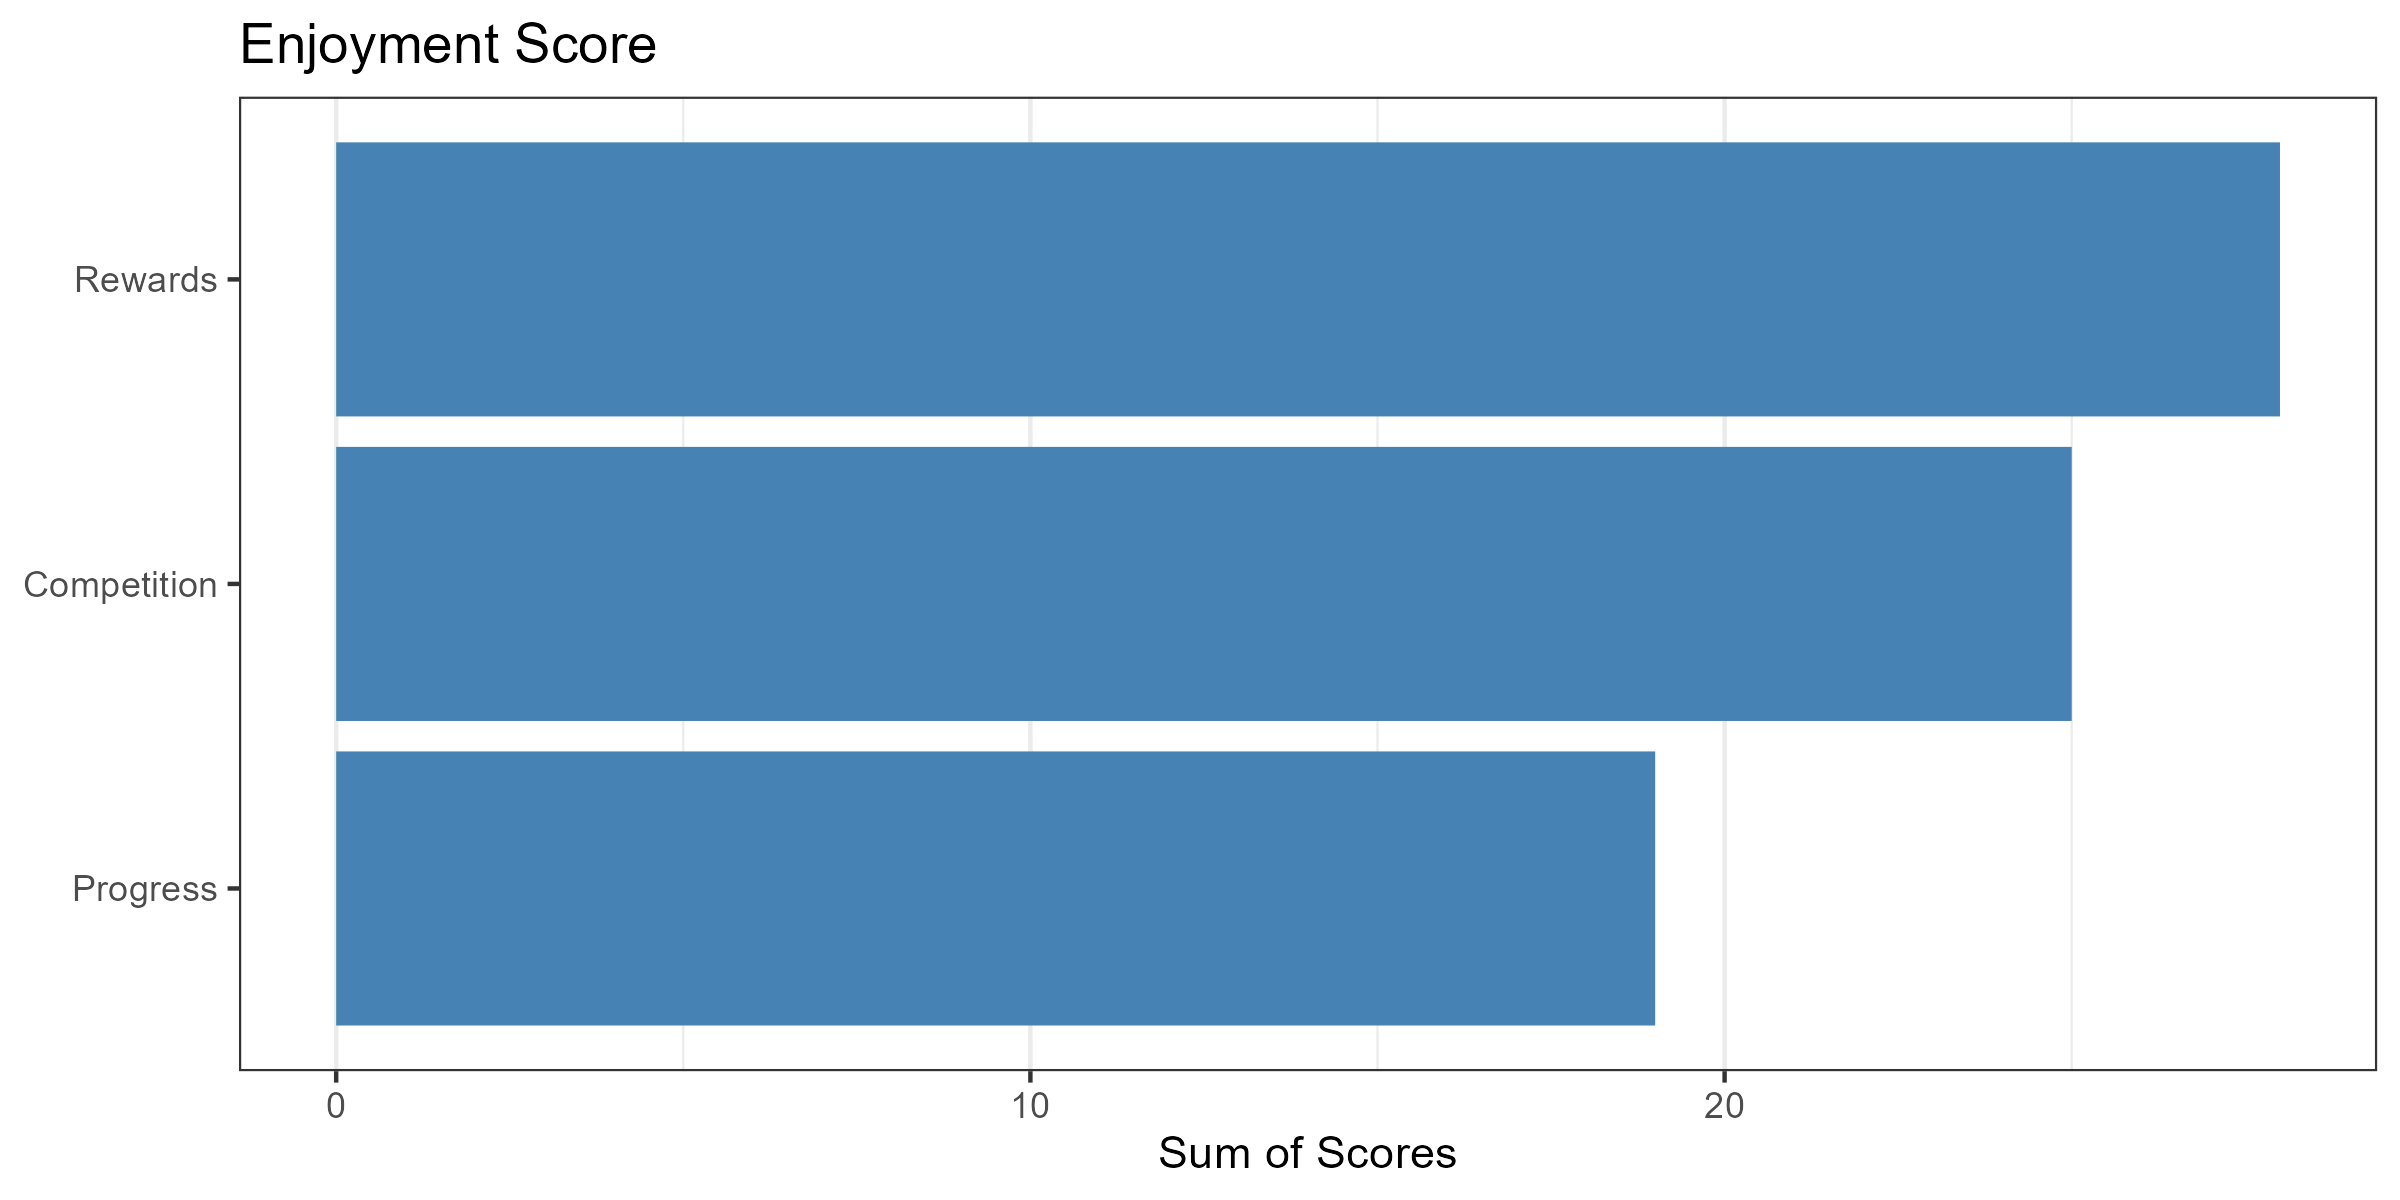
\includegraphics[width=\linewidth]{Template_Latex_ScuDo_Tesi/Chapter3/proto_rq3_enj_versions.png}
        \caption{Distribution of the Enjoyment Score for the three prototype versions}
        \label{fig:proto_rq3_enj_versions}
    \end{subfigure}\hfill
    \begin{subfigure}{0.9\linewidth}
        \centering
        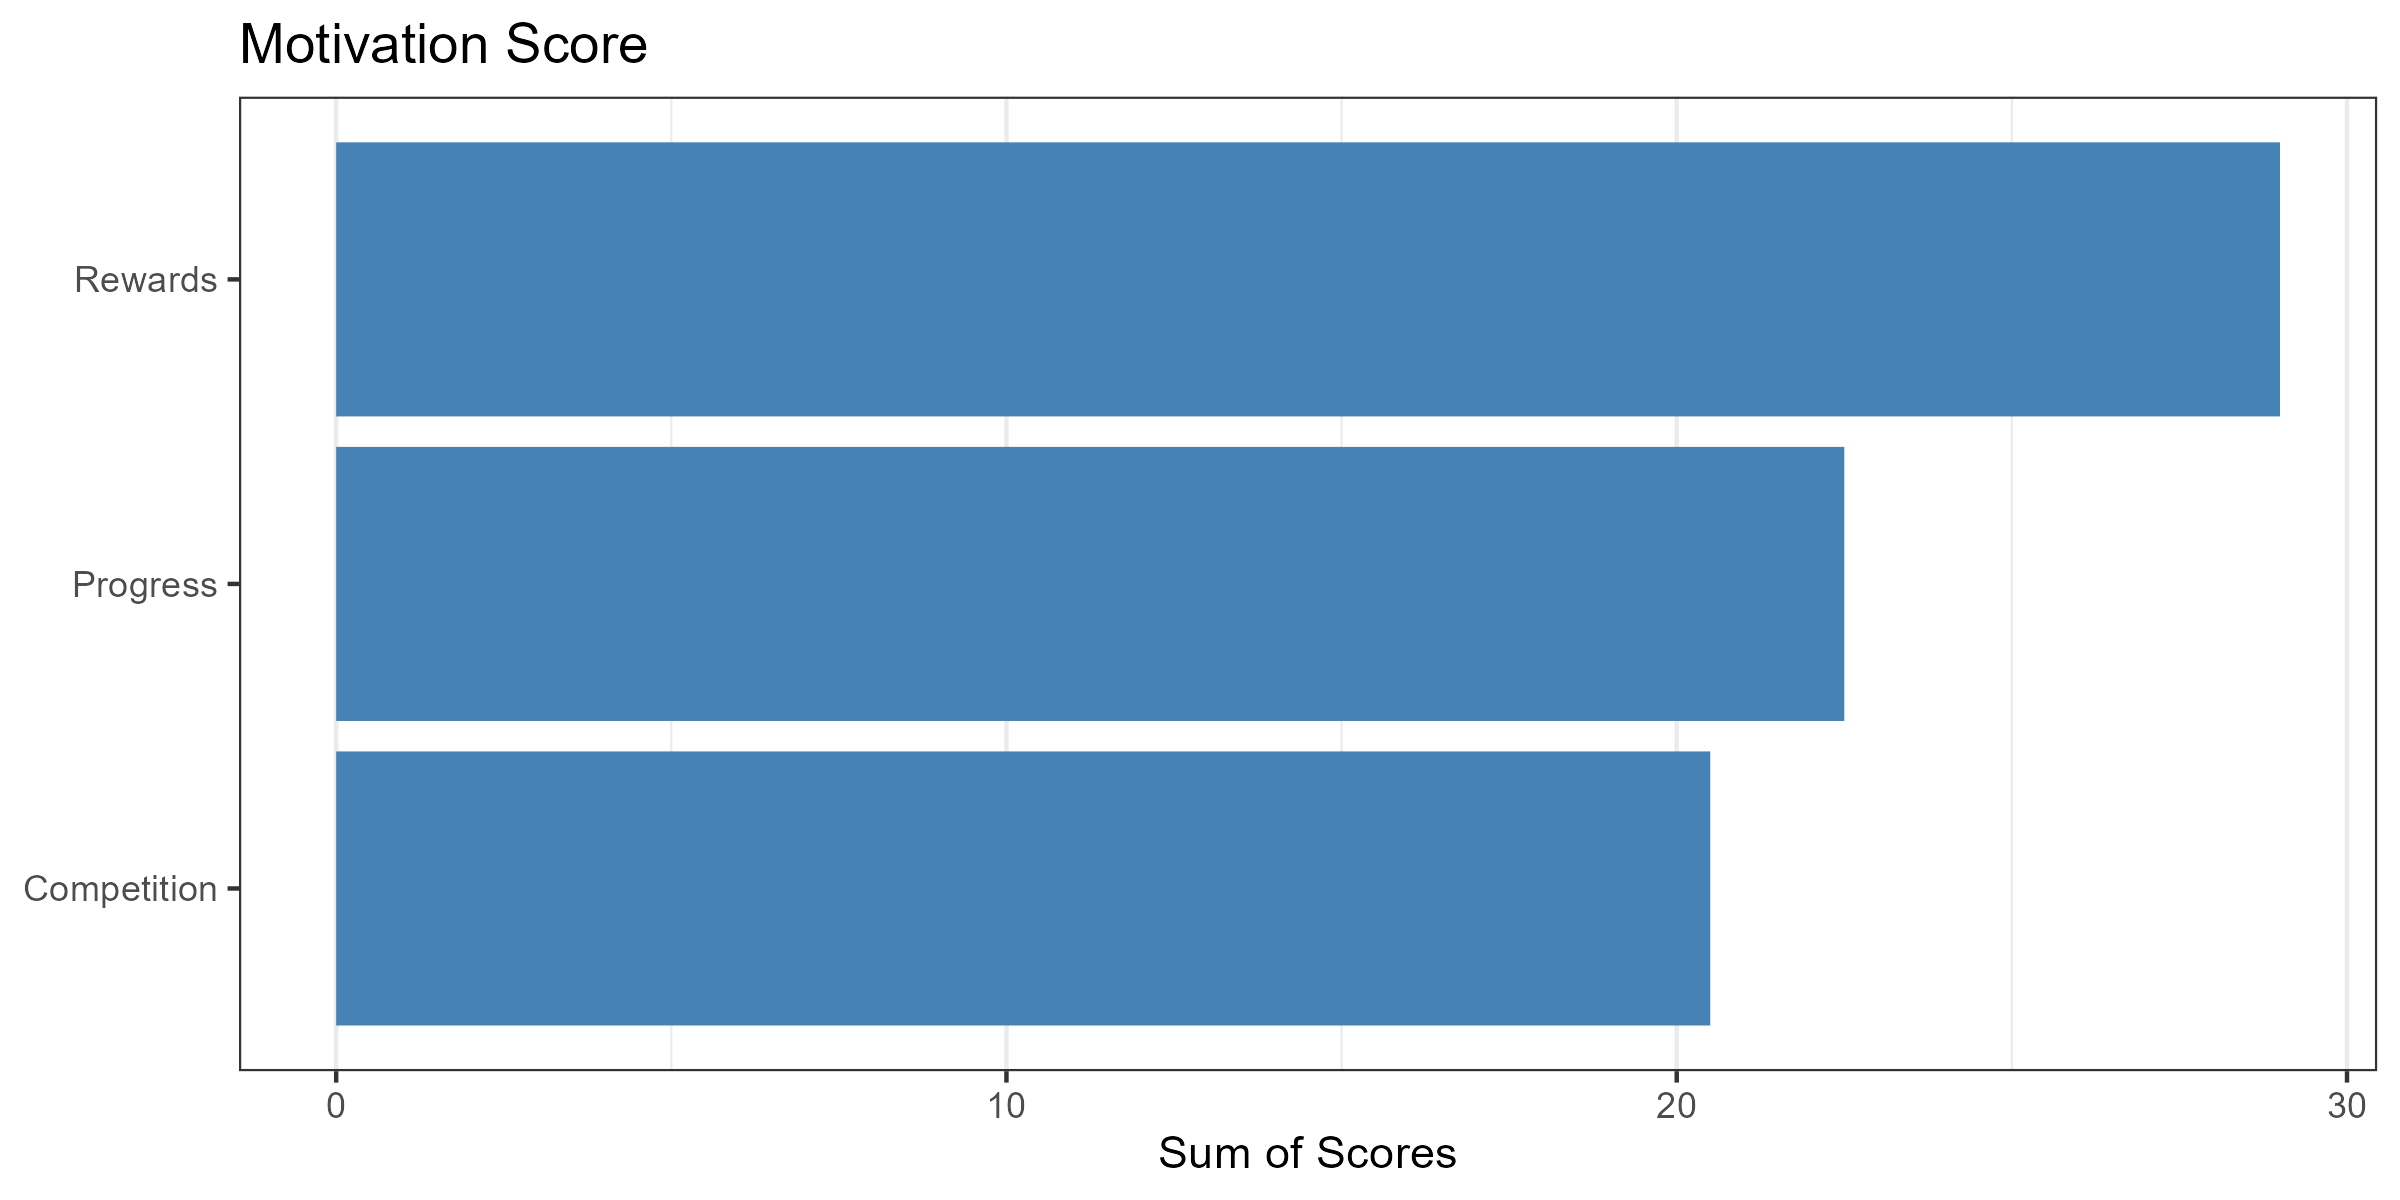
\includegraphics[width=\linewidth]{Template_Latex_ScuDo_Tesi/Chapter3/proto_rq3_motiv_versions.png}
        \caption{Distribution of the Motivation Score for the three prototype versions}
        \label{fig:proto_rq3_motiv_versions}
    \end{subfigure}
    \caption{Scores assigned to the three game versions in the post-study survey}
    \label{fig:proto_rq3_version}
\end{figure}

Overall, the \textit{Rewards} version emerged as the winner of these two comparisons as well, gaining a total of 28 Enjoyment Score and 29 Motivation Score, while the remaining two versions presented some differences in their ranking: the \textit{Progress} version was judged as the second most motivating one with a score of 22.5 but as the least enjoyable, scoring only 19, while the \textit{Competition} version got an enjoyment score of 25 and a motivation score of 22,5. This result further confirmed the position of the \textit{Rewards} version as the best received out of the three, implying that further development of BIPMIN would have needed to consider the elements present in said version as the starting point.

Additional questions on the survey aimed at constructing the participants' ranking of the game mechanics, to identify which were the most appreciated and perceived as most motivating and enjoyable, to build on them with the goal of creating a complete version of BIPMIN.

The first question related to the game mechanics asked participants to state whether they would have liked the mechanic to return or not in a complete version of the game used in a classroom environment; the sum of the preferences expressed by the participants was computed to retrieve a score that would give the appreciation of the various mechanics. Figure \ref{fig:proto_rq3_pref_mechanics} displays the distribution of these preference scores. 

\begin{figure}[H]
    \centering
    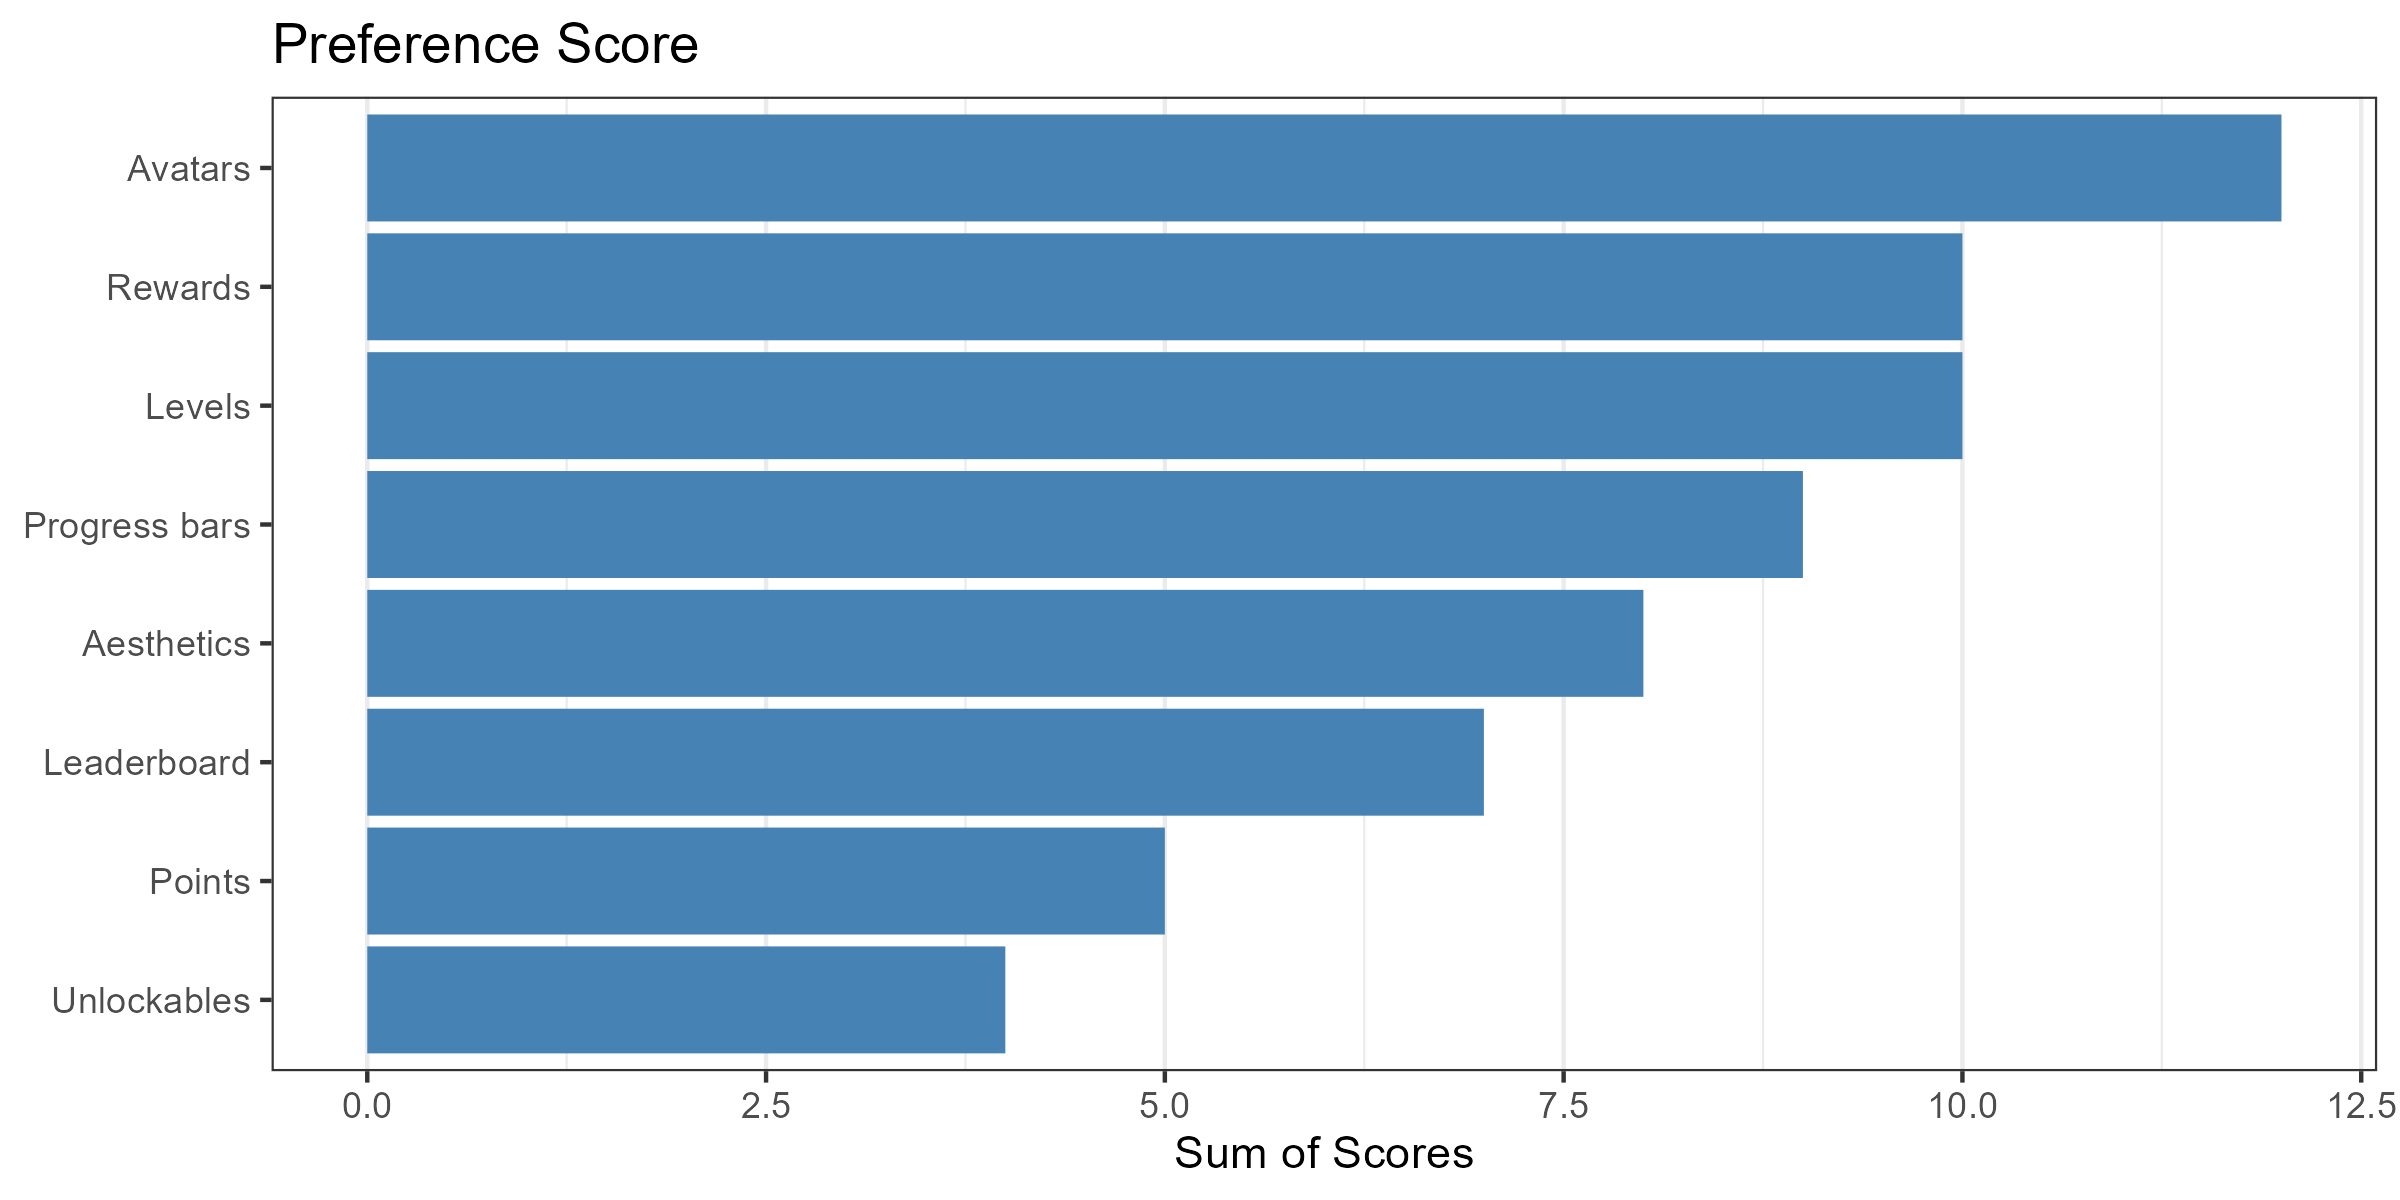
\includegraphics[width=1\linewidth]{Template_Latex_ScuDo_Tesi//Chapter3/proto_rq3_pref_mechanics.png}
    \caption{Preference scores assigned to the eight game mechanics}
    \label{fig:proto_rq3_pref_mechanics}
\end{figure}

In an unexpected contrast with the results obtained by the \textit{Progress} version, its mechanics did not score as favorably: while rewards were appreciated by almost all participants (10 out of 12), unlockable exercises were not as requested to be kept for a complete version; a possible interpretation of this result is that locking exercises behind progression may not be as appreciated if the application is to be used over multiple lectures and sessions, as it would reduce the ability for users to play and try different exercises. A second surprising outcome is the fact that avatars, a mechanic present only in the \textit{Competition} version, was appreciated by all participants: the interpretation is that avatars provide freedom for users to express themselves, and with the perspective of unlockable avatars and the ability to display them to a classroom of peers, participants may enjoy playing with them the most. Other mechanics such as levels and progress bars were also appreciated by at least 75\% of the participants, implying the possible positive reception of titles tied to progression and visual indicators of success and correctness for the exercises.

The two other questions that focused on the game mechanics aimed at measuring the \textit{Enjoyment Score} and \textit{Motivation Score} for them, by asking participants to rank them from 1 (least enjoyable/motivating mechanic) up to 8, with the scores being computed as the sum of rankings given by all participants. The resulting scores are shown in Figures \ref{fig:proto_rq3_enj_mechanics} and \ref{fig:proto_rq3_motiv_mechanics}.

\begin{figure}[H]
    \centering
    \begin{subfigure}{0.9\linewidth}
        \centering
        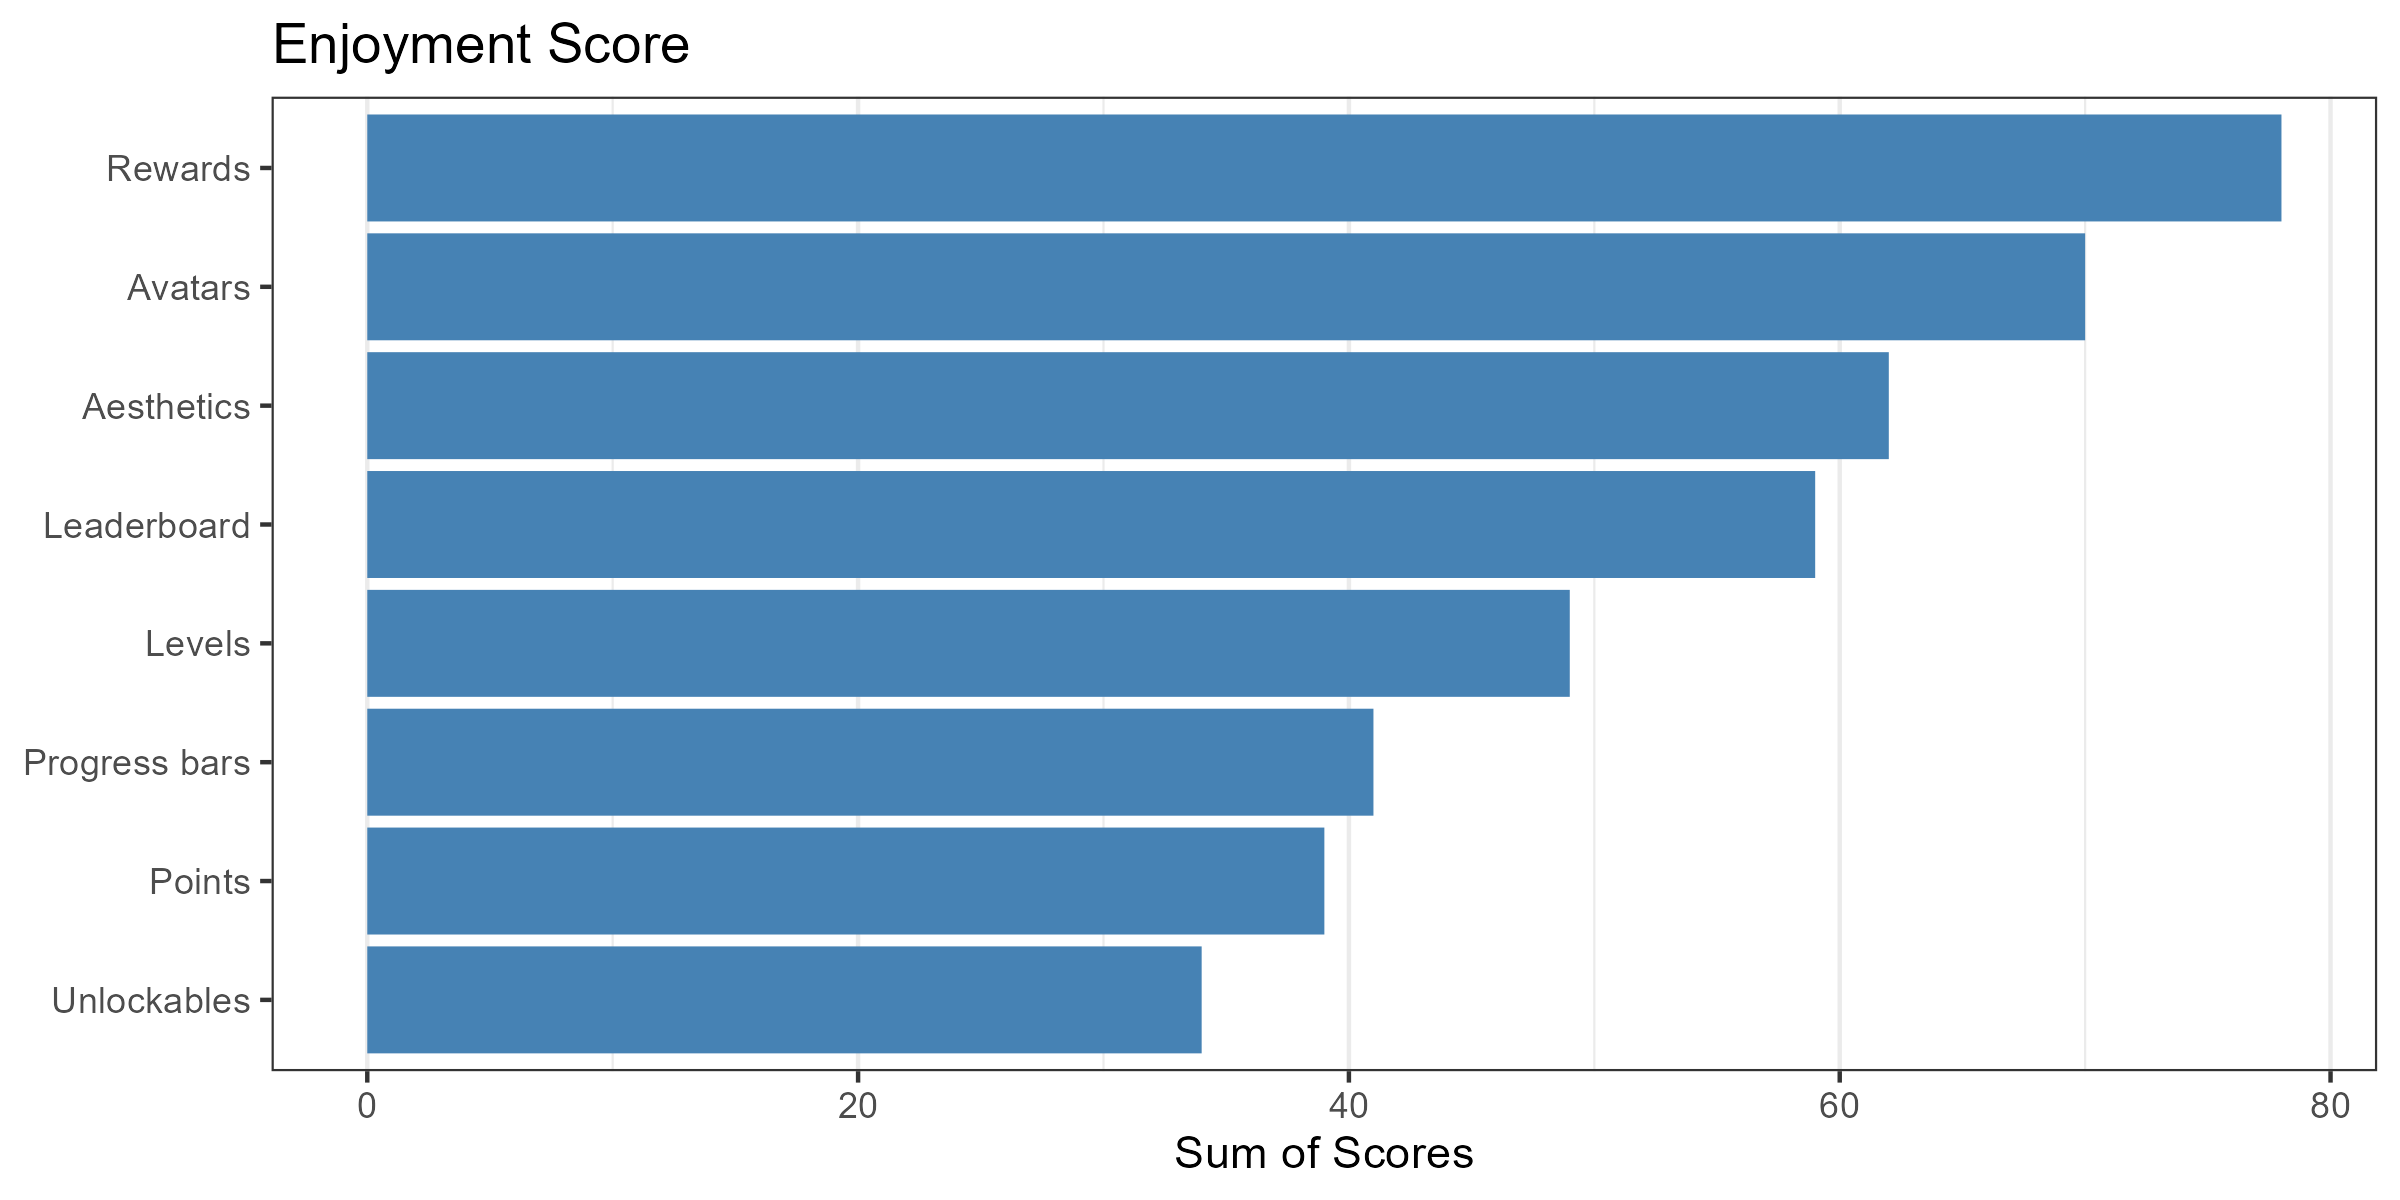
\includegraphics[width=\linewidth]{Template_Latex_ScuDo_Tesi/Chapter3/proto_rq3_enj_mechanics.png}
        \caption{Distribution of the Enjoyment Score for the eight game mechanics}
        \label{fig:proto_rq3_enj_mechanics}
    \end{subfigure}\hfill
    \begin{subfigure}{0.9\linewidth}
        \centering
        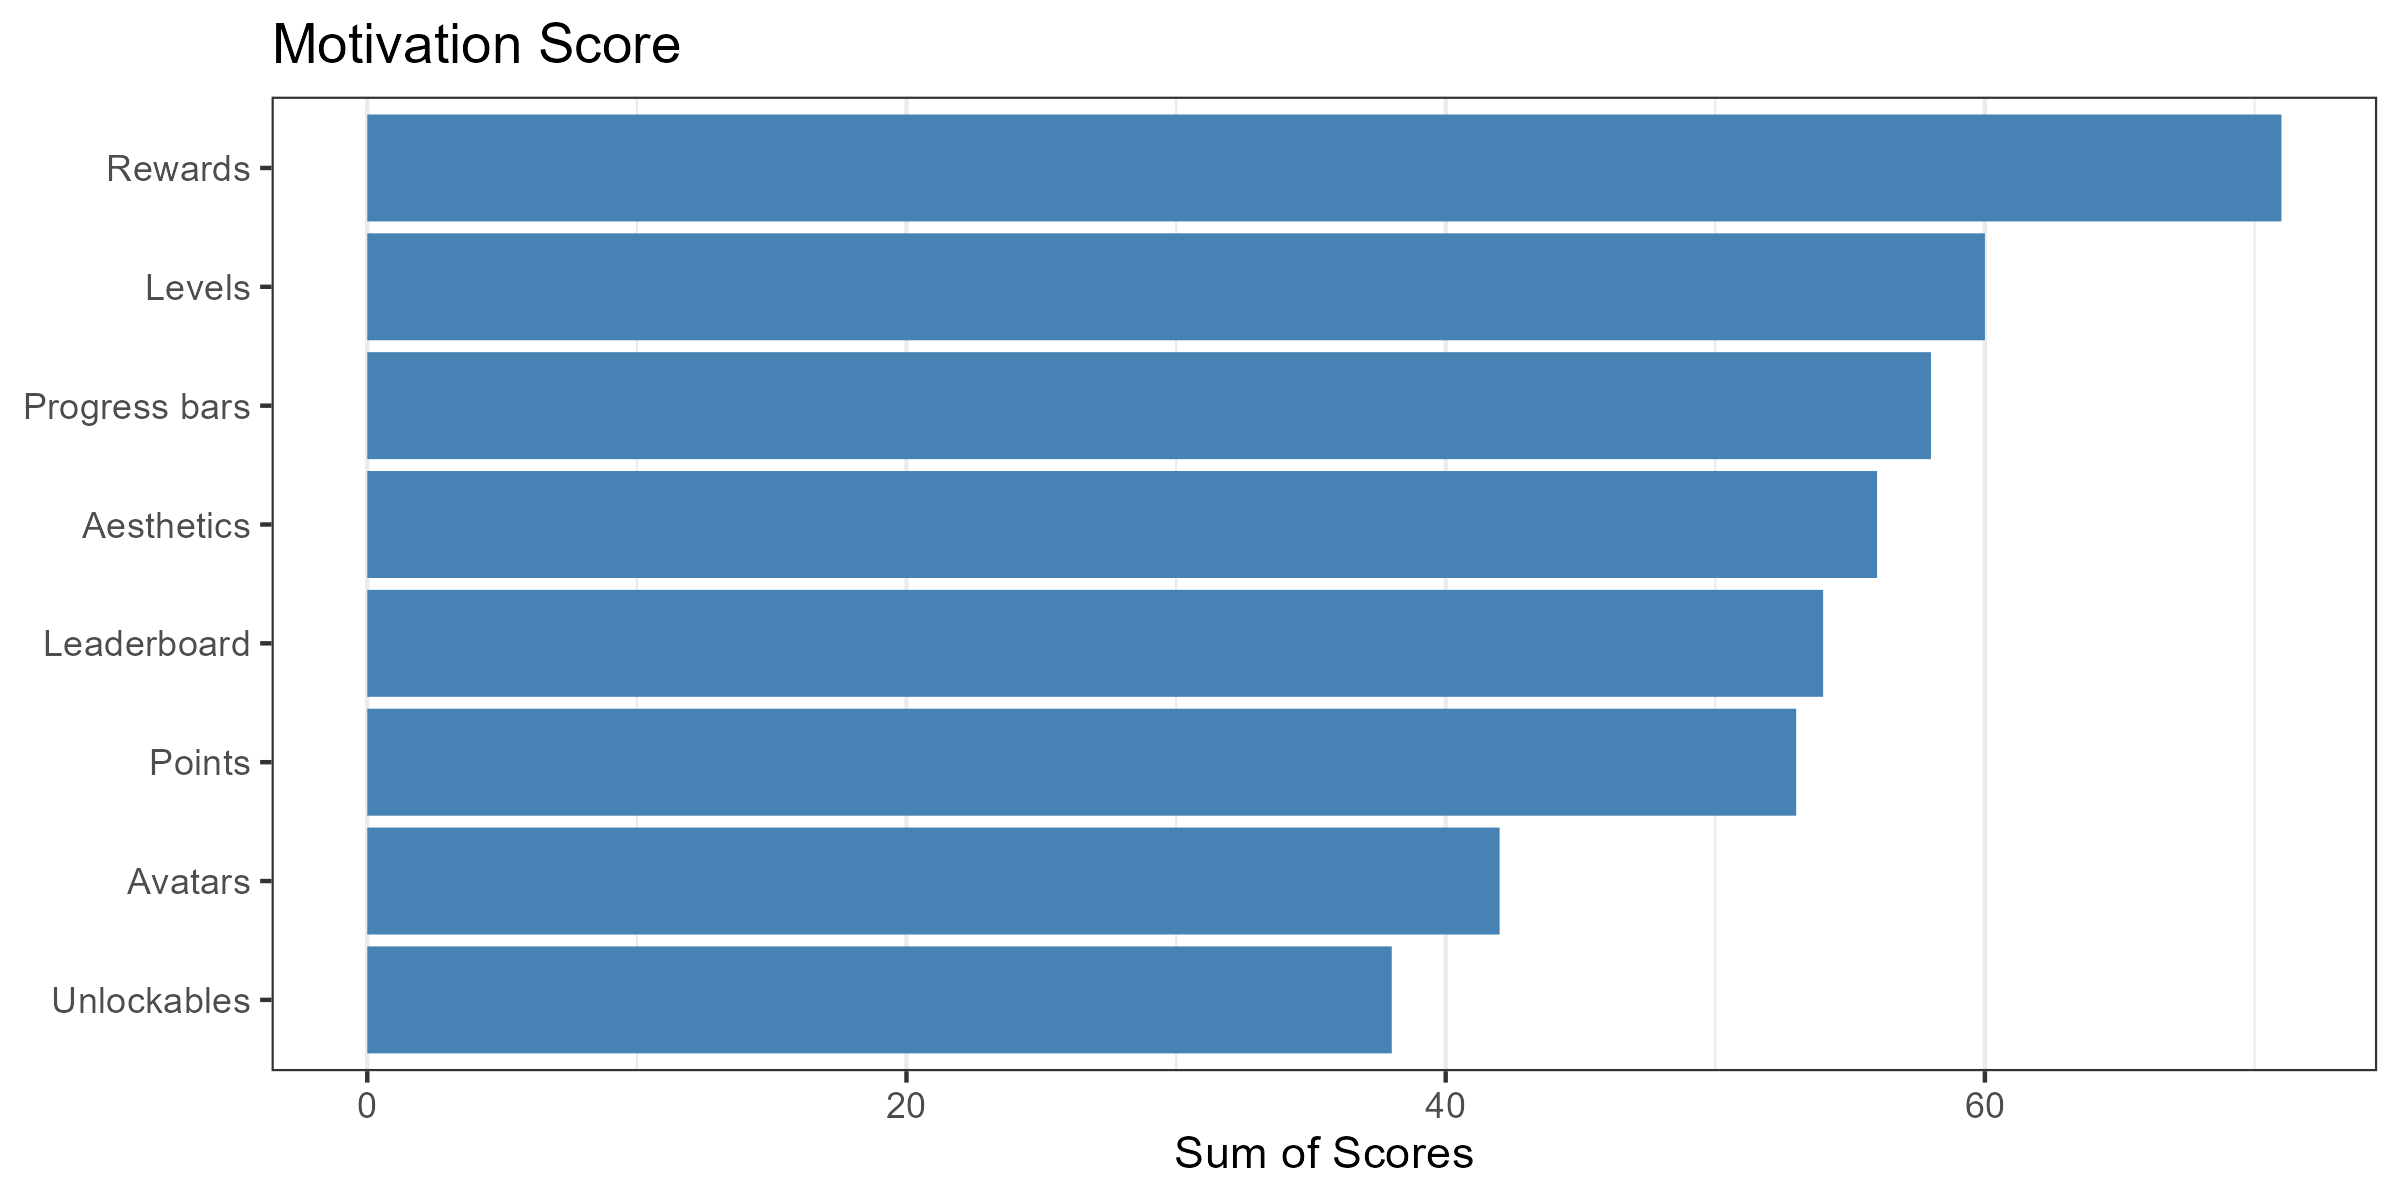
\includegraphics[width=\linewidth]{Template_Latex_ScuDo_Tesi/Chapter3/proto_rq3_motiv_mechanics.png}
        \caption{Distribution of the Motivation Score for the eight game mechanics}
        \label{fig:proto_rq3_motiv_mechanics}
    \end{subfigure}
    \caption{Scores assigned to the eight game mechanics in the post-study survey}
    \label{fig:proto_rq3_mechs}
\end{figure}

Regarding the enjoyment score, rewards were considered the most engaging mechanic, obtaining a total score of 78 and being ranked as the highest by 4 out of 12 participants, strengthening even further the positive perception of this mechanic; other appreciated mechanics were avatars, with a score of 70, then aesthetics with 62 and the leaderboard with 59. In line with the results tied to the preference of mechanics, experience points and unlockable exercises ranked as the least enjoyable mechanics. It can be assumed that these mechanics may be better perceived in a long-term environment, where students can better appreciate the impact of leveling up and unlocking new elements.

Regarding the motivation score, rewards were again confirmed as the best received mechanic, ranking first with a total score of 71 and 5 participants considering it the most motivating mechanic; other well-received mechanics in this aspect differed from the enjoyment score, with levels and progress bars being considered the second and third best mechanics, with 60 and 58 points respectively. The takeaway from this resulting ranking is that these two mechanics, while not being perceived as particularly enjoyable or fun, acted as a strong motivating force, with a sense of personal growth being tied to successful exercise completion and visual feedback for following correct modeling practices. On the other hand, unlockable exercises were also confirmed as the lowest ranking mechanic, implying that a full version of BIPMIN could benefit from the removal of this particular mechanic, or at least from a rework so that other elements are unlocked instead. 

Another mechanic that was not perceived as particularly motivating was the use of avatars: this result feels surprising, considering that they were the mechanic with the highest preference score and second highest enjoyment score; a possible explanation may be the fact that all avatars were unlocked by default and thus, while the ability to select a stylized animal to represent oneself was perceived as fun and interesting, there were no other changes to the mechanic over time, implying that the feeling of novelty could have worn off quickly. A way to strengthen this mechanic could be to change the set of avatars so that not all of them are available immediately, and some of them can only be unlocked over time, tying the concept of avatars and unlockable elements together.

The survey also included an open question where participants could leave comments regarding feedback or suggestions to improve the prototype: only half of the participants answered this question, and their comments included suggestions such as the inclusion of a BPMN tutorial, the addition of an achievement system, the creation of a one-on-one competition mode, and the conviction that the leaderboard could be useful in a classroom environment, despite the participant themselves noting they were not a competitive person.

Additionally, many of the participants expressed opinions throughout the trial focusing mainly on the \textit{Competition} version, which was not perceived as favorably as the \textit{Rewards} one; however, the participants noted that the version would have probably been perceived differently if used during a course, noting that they would have liked to compete with their colleagues. The fact that trial sessions were conducted independently of one another may have had an impact on the low appreciation of the \textit{Competition} version, meaning that the mechanics that it employed may be more impactful if used over a longer period and with students being able to interact with each other while using the tool.

\answer{RQ3}{The \textit{Rewards} version was considered the most preferred, enjoyable, and motivating version out of the three, with the reward in the form of puzzle pieces being perceived as the most enjoyable and engaging mechanic; the other game mechanic implemented in this version, unlockable exercises, was not perceived as favorably, however, implying that unlockable elements could still be effective, but may need to be refined into other elements such as avatars or badges. The design of the study as a set of independent single-sessions may have impacted the perception of the \textit{Competition} version, with its mechanics perhaps being better-received in a long-term classroom environment.}



\subsubsection{Threats to validity}
\label{sec:threats}

The threats to the validity of study are discussed in line with the four categories reported by Wohlin et al.\cite{wohlin2012experimentation} and discussed in Section \ref{sec:empirical_methods}.\\

\textbf{Threats to internal validity:} for the trial study, threats to internal validity are related to how the BIPMIN prototype was designed and regard mostly the game mechanics that were implemented: these mechanics were selected since they were among the most commonly used and discussed in gamification literature, with known potential benefits and drawbacks. There is no guarantee, however, that the mechanics that were implemented are actually the most beneficial, or that other mechanics could have been more effective. 
A similar reasoning applies to how the mechanics were grouped in three different versions: the results may have been different if the three versions included different mechanics, for example, or a different combination of the existing ones.

Finally, the implementation of the evaluation engine could also qualify as a potential threat, since it only assesses the syntactic quality of a diagram and limits the semantic aspect to checking whether specific elements are present or not, without any check on their order or actual textual content. The fact that not all aspects of BPMN modeling rules are covered by the evaluation engine could affect the impact of BIPMIN on student performance.

\textbf{Threats to conclusion validity:} rhe main concern on this aspect is the fact that this study was a preliminary evaluation focused mainly on the usability of the prototype and on the perception of the game mechanics. The results and the conclusions gathered after the study may not hold after a future empirical evaluation of BIPMIN more focused on the educational aspect of gamification impacting BPMN modeling education.

Additionally, the time constraints in the study, as well as the design of the study as a single session, could possibly affect the evaluation of both the \textit{Progress} and \textit{Competition} versions: for the former, the study being composed by multiple small tasks means that it is not easy to evaluate progression fully, and multiple tasks supplied over time may be more effective. A similar reason applies for the second version, since single and independent sessions are not suitable to evaluate leveling mechanisms and leaderboards, that conventionally better appreciated over longer time periods.

\textbf{Threats to external validity:} this study was designed as a preliminary evaluation of a prototype gamified educational tool for process modeling focused specifically on BPMN. The results cannot be generalized to other process modeling notations, to non-educational context where BPMN can be employed, or to educational contexts focused on other topics. Furthermore, the results cannot also be generalized depending on the selected game elements and mechanics, meaning that results cannot be compared to those that other approaches, focused on different game mechanics, could obtain.

\textbf{Threats to construct validity:} for this study, the metrics that have been measured (e.g., enjoyment and motivation scores, time spent completing tasks, preferred versions and mechanics) have not been mapped to the effectiveness of BIPMIN as an educational tool, meaning that its effectiveness on improvement of student performance is still not known.

\subsection{Key findings and lessons learned}

This first research activity had the goal of developing the prototype for a gamified educational application focused on BPMN modeling. The prototype was implemented with three different versions centered around themes (rewards, competition, progress), each with specific game mechanics in place to distinguish the impact of the three themes. A preliminary evaluation focused on the usability, the potential benefits in modeling performance, and the perception of the game mechanics was performed, involving 12 Masters' students.

The preliminary trial showed that the prototype achieved a good usability score, measured via the System Usability Scale, implying a good design to use as the starting point for an effective educational application; part of the analysis focused on the performance showed that students were, on average, able to complete their assigned modeling tasks within the expected time period, and were able to understand the provided feedback and reduce the number of attempts needed to reach successful exercise completion. The gamification aspect was well received, with the version focused on rewards being the most appreciated of the three.

Overall, the evaluation showed that gamification of BPMN modeling can be well received by students, with many participants stating that they would have liked to have something similar to BIPMIN when learning BPMN: the positive reception warrants a continued development of the prototype to ensure it can be used to enhance classroom activities. Something that should be considered, however, is how some of the mechanics have been received by the participants: competition elements such as experience points and the leaderboard were noted to have been less appreciated due to the study being performed as a single session with no interaction among students, implying that these mechanics would be more suitable for long-term usage.

Another mechanic that was less favorably received was the use of unlockable exercises: while it belonged to the most appreciated version, the one focused on rewards, this mechanic was considered neither motivating nor enjoyable by the participants; the interpretation is that using unlockable elements could potentially be more appreciated by the users of the BIPMIN application if those elements were not exercises, which are necessary to proceed, but rather tangible rewards such as the puzzle pieces that were used in the prototype. A possible improvement of the platform that builds on the best-received version could be the introduction of achievements and badges, or possibly the use of more unlockable avatars, a mechanic that was considered among the most enjoyable ones but one of the less motivating, perhaps due to the fact that avatars were all available since the start of the trial.

Lastly, the main point of concern after the end of the preliminary study is perhaps the most significant one: the current state of the BIPMIN tool offers very little in terms of actual educational benefits, since the application is considered fun and motivating by students but does not offer a way to learn good modeling practices in terms of semantic validity. The evaluation engine, in its current implementation, is able to tell whether a diagram contains the necessary elements and their connections, but is not able to tell whether these elements are in the intended order, for example, or if the element has the intended meaning: for example, given an exercise focused on a food delivery application, a solution might expect a start event followed by task related to ordering a dish. The evaluation engine would be satisfied as long as those two elements were present, even if the task stated a completely different activity.

\articleSummary{
color1
}{
Summary of the BIPMIN prototype study
}{
The preliminary study on the BIPMIN prototype showed that gamification of BPMN modeling can be well received by students, with mechanics that give tangible rewards being preferred over others that are more suitable for long-term use. The most obvious limitation of the prototype is the absence of semantic evaluation of the produced solutions, an issue that needs to be addressed before revising the implementation of game mechanics. Regarding the three versions, although one has emerged as the clear favorite, the remaining two also showed some possibly effective elements, meaning that future development should consider a combination of multiple mechanics, rather than develop just a single version. 
}



\section{Revisal of the first prototype}

Following the results of the first preliminary study on the prototype, a development cycle focused on improving the tool started in November 2022. The goal of the development process was to create a new version of BIPMIN that could be used to perform an empirical study to identify whether gamification could help students improve their BPMN modeling practices compared to standard modeling approaches, rather simply being perceived as a fun and motivating activity.

For this purpose, the prototype had to be changed according to two main requirements: extending the evaluation engine so that it could also identify semantic errors in a student diagram and assess the actual content of the elements (names and labels) rather than just the element types, and selecting a subset of the existing game mechanics to merge all three versions into a single one.

\subsection{Enhanced evaluation engine}

To improve the evaluation engine, the first necessary step was to define a way to ensure semantic errors could be identified in an automated way, with the end goal of creating a mechanism that would simulate the evaluation process performed by a human when supplied with a BPMN diagram to evaluate. The target evaluation process was the one where a teacher looks at a diagram drawn by a student and identifies which expected elements in the solution are present or are missing, which ones belong to the correct pool or not, which ones are placed in the wrong order, and which ones have the wrong type. 

To execute this evaluation procedure through an automatic evaluator, it was necessary to define a way for the evaluator to know which elements a diagram was supposed to contain, their types, their expected meaning, their position in pools and lanes, and their order relative to the rest of the process; all this necessary information would serve as the baseline for the evaluator, by giving it data that a student's diagram would be compared to. 

The necessary data and information was thus defined in the form of the \textit{Reference Solution}, a structure that would represent a BPMN diagram containing all the necessary elements in their correct form and order. The definition of this structure came after observing the way modeling assignments are handled in practical laboratories in certain courses at Politecnico di Torino: students are expected to solve practical exercises on their own at first, and an example of a valid solution for those exercises is then drawn and explained by the course professor at a later date, providing guidance on how to represent certain constraints and what are the possible errors that can happen when modeling the exercise's requirements.

The improved automated evaluator would simulate the scenario where a teacher looks at a student's diagram and, while knowing the intended reference solution, compares the student's diagram to the expected one, and provides feedback by explaining which elements are correct and which ones are not. For elements to be considered correct, they would have to be equivalent to those in the reference solution and appear in the same order in the diagram: for example, given an exercise about a system for handling internship registrations for a university with its reference solution expecting the first element to be a task where a student chooses an internship proposal, the evaluator would consider this requirement to be correctly represented if a diagram included a task with a name/label that expresses the same meaning.

Given the variable nature of BPMN modeling, with its multiple types of elements and alternative ways to represent the same set of requirements (e.g., an exchange of information between participants could be represented with either message events or message tasks, notification could be represented as either service tasks or with message exchanges between an actor and an external pool), the automated evaluator would also need to consider possible alternative representations, not limited to simply considering the different possible names of elements, but also their types and combinations as well. 

Another serious point of concern came from the order the elements would take in the process: considering the fact that requirements could be represented in various ways, and that requirements come in a fixed order, the need to represent subsets of the full set of requirements for modeling exercises was identified as the key challenge in the development of the improved evaluation engine.

The solution that was found to address this need was the introduction of the conceptual division of the set of requirements, with the corresponding sections of the reference solution, into \textit{Process Parts}: similar to how a student would read paragraphs of an exercise's text and, as they identify a specific requirement, draw the corresponding element or elements in the diagram, the evaluator would need to define data structures containing the necessary information to represent the various requirements in BPMN format. The evaluation procedure activated by student input would then iterate through the submitted diagram, looking for elements that match the requirements specified by the data structures, giving feedback and updating the game mechanics according to the student performance.

The definition of process parts was implemented in a similar way to the six evaluation criteria that were implemented in the prototype by keeping JSON as the selected notation to express the necessary information for the required BPMN elements, with keys representing the process parts and values being used to define the criteria to satisfy to correctly model the process part. Keys were structured using the notation \textit{$E_t\_P_n$}, where \textit{$P_n$} is used to represent the name of the given process part and \textit{$E_t$} specifies whether the process part contains one element (in which case it will be equal to the element type following the \textit{bpmn.js} specifications) or multiple connected ones (in which case it will be \textit{GroupRules}). The naming structure for defining process parts also acts as the first condition to check: in case a process part is represented by a single element, subsequent checks defined by the values in the JSON will be performed only elements of said type; if, instead, a process part is composed of multiple elements the corresponding value will be a list of objects with element types as keys and objects with criteria as values, with checks being made only on elements with the same type as the inner keys.

%\GG{magari immagine/tabella/altro con mapping testo <-> elementi?}

The evaluation procedure which, similarly to how it was done in the prototype version, is activated by students choosing to have an automated assessment of their diagram, works by iterating through all process parts defined for an exercise and checking if there is an element (or group of elements) with the corresponding type that satisfies all criteria associated with the process part. These criteria are defined to represent the various conditions that are checked during a human-led BPMN evaluation and, as a consequence, should be checked by the evaluation engine; two conditions apply in all scenarios and are thus always checked:

\begin{itemize}
    \item An element represents a process part if its name conveys the intended meaning. For example, a process part where a given actor needs to verify a document is represented if a task's textual content contains a verb that expresses verification and the noun \textit{document} (or a valid synonym). In the evaluator, this condition is represented by defining an attribute in the process part's data structure named \textit{Label}: this attribute is a list of strings, and the condition is verified if there is an element of the required type whose label contains at least one of the specified strings.
    \item An element is considered valid if it belongs to the expected pool. This condition has an associated attribute in the data structure named \textit{Pool}, which is a list of strings; the condition is satisfied if the target element belongs to a pool whose name contains at least one of the strings in the list.
\end{itemize}

Other conditions concern the relationship between process parts, which is an additional important element to consider during a human evaluation: to represent a process part, it may not be sufficient to have an element with the correct name and in the correct pool, the order of requirements is also something that impacts the correctness of a diagram. Assuming that two requirements are specified one after another in the process description and, consequently, their chronological order also sees one come after the other, the corresponding elements in the diagram must also come one after another. As a consequence, process parts in the reference solution can also specify the information relative to the process part that comes immediately before or immediately after with the use, respectively, of the \textit{Parent} and \textit{Target} labels. The data structures associated with these labels are objects that work in the same way as the structures that define the elements for the process parts, meaning that they have their own \textit{Label} attribute, to specify the strings a preceding/following element is expected to include in its label, as well as an attribute called \textit{Element}, that specifies the type of element. If an element specifies conditions related to its preceding/following element, then it must be preceded/followed by an element that satisfies its inner condition, and it must satisfy its own condition as well.

Additionally, other criteria have been defined to cover conditions related to specific elements: for example, event types (e.g., timer, message, error) are defined through a specific attribute in the corresponding object instead of being separate object types; to cover this requirement, event elements have an additional constraint called \textit{EventDefinition}, requiring events to also have the corresponding definition to be considered valid, in addition to other constraints.

Other criteria concern boundary events, a special type of events that can be appended to tasks to signify non-standard process execution in case the event's condition is verified before the task terminates. To represent a process part that involves this type of events, both the event and the task need to have additional definition: for the former, an attribute called \textit{BoundingElement} is used in the same vein as the constraints that specify preceding/following elements, by listing the conditions that the element a target message is attached to must satisfy; an additional condition for boundary events depends on whether they are interrupting (if the event activates then the bounding task can never proceed and the process continues from the event) or not, with the boolean attribute \textit{Interrupting} stating whether the event under evaluation needs to be interrupting or not.

Message exchanges may also be considered required conditions in some cases: if two elements exchange messages they will have attributes \textit{MessageSender} or \textit{MessageTarget} that specify the condition of the element the message is received from, or is sent to, respectively. In case an element has one of these conditions, it will be considered valid for its process part if it exchanges a message with an element that satisfies the inner properties.

%\GG{una volta fatto l'esempio con mapping testo -> parte, fare esempio parte -> regole}

The reworked version of the evaluation engine addresses its main limitation with the original implementation, that is, the inability to evaluate the semantic quality of a diagram: with the definition of a mechanism that checks for process parts and assesses whether a diagram contains the required elements, BIPMIN can now be used to give detailed feedback when students ask for an evaluation of their diagrams. Furthermore, the ability to check for syntactic quality is still implemented with the same library that was used in the prototype (\textit{bpmnlint.js}), ensuring that the feedback covers both best practices about modeling rules and ability to represent the intended domain; pragmatic quality, however, remains something that is complex to automatically evaluate, since it focuses more on the readability and understandability of a diagram, features that are better assessed via human evaluation. The new version of the evaluation engine only assesses the content of the various elements and their position in the process flow in relation to one another, with no focus on the elements' positioning in the available space or their size; naming conventions are also not strictly enforced, since the only check on element labels is on ensuring that specific, context-defining words are included. 


\subsection{Selected and revised game mechanics}

Building on the results of the preliminary usability trial, the second main point of development was the selection of the game mechanics to keep in the revised version of BIPMIN. The first decision was to move away from the division in three separate versions and merge them into a single tool that supports multiple kinds of game mechanics. Additionally, the goal for the improved version of the tool was to conduct an empirical study with a large cohort of students to assess the educational impact of gamification on BPMN modeling; this decision guided the selection of game mechanics, with a focus on mechanics that could be most effective into a single-use session, as well as those that could be helpful in guiding students toward producing correct diagrams with the support of the improved evaluation engine.

Following this decision, all mechanics implemented on the prototype had been reanalyzed to decide if they were going to be considered for development for the revised version focused on the study, or if they were going to be focused on when developing a version of BIPMIN focused on long-term use:
\begin{itemize}
    \item The leaderboard, which had been described by multiple participants in the pilot study as a mechanic that would have been more successful if used in an actual classroom environment.
    \item Experience points, which were something that built up over multiple exercises in the prototype, were discarded due to being related to the leaderboard, and thus judged as more suitable for a long-term study where students could solve multiple exercises.
    \item Avatars, despite being well-received in the pilot study, were tied to the leaderboard and, in general, are a mechanic that relies on interaction between players to be appreciated. A decision was taken to combine avatars and unlockable elements in a future version of the tool, more focused on long-term use, in case the results of the empirical study proved the effectiveness of gamification on learning modeling practices. 
    \item Progress bars were implemented in the prototype for the progression in a single exercise, as well as the progression over all the available exercises. The progression of a single exercise was kept, as a way to help students easily understand how close they were to reach exercise completion.
    \item The skill level, in a similar fashion to experience points, was considered something that could have a better impact if used over time;
    \item Prizes were the overall most appreciated game mechanic, and were considered as a mechanic that needed to be kept, with them being considered both the most enjoyable and motivating mechanic. Although the original implementation used multiple exercises to provide the available puzzle pieces as rewards, this mechanic was deemed to be easy to implement in the execution of a single exercise.
    \item Unlockable exercises were the least appreciated mechanic in the prototype's evaluation, and were already considered for a rework after the analysis of the trial's results. Due to unlockable elements being something that reflects learning progression over time, it was decided that such a mechanic was not needed for the planned study.
    \item The overall aesthetic of the application was also evaluated as a mechanic in the pilot study, and was somewhat well-received. The graphical feel of the application was thus kept, even with the combination of multiple versions into a single one; however, it was decided that the aesthetic aspect of the tool was not going to be considered a game mechanic for the empirical evaluation, focusing exclusively on the actual game mechanics that could have an impact on the learning experience, rather than on the app layout and look.  
\end{itemize}

After having selected progress bars and prizes as mechanic, it was decided to refer to them during development and analysis by considering their original themes in the prototype, as they better encompassed the intended meaning of the mechanics; thus, the new version of BIPMIN had to implement mechanics related to \textit{Rewards} and \textit{Progress} that could support learning modeling practices. By selecting these two mechanics for implementation, BIPMIN was envisioned as a tool where students could solve modeling exercises by knowing how much of the intended process representation they were covering and they would get rewarded by following modeling rules and representing parts of the target domain; other mechanics had to be selected with a focus on further strengthening the educational aspects, as well as being easy to blend together with the new evaluation engine. 

To blend together the game mechanics with the evaluation engine, it was decided to turn the output itself of the automated evaluations into a game mechanic, leading to the definition of the \textit{Feedback} mechanic, reinforcing the interpretation of the automated engine as a simulation of the explanation that a teacher gives when evaluating the diagram; at this point, however, the game mechanics were going to provide an imbalanced experience according to the tenets of the Octalysis framework, focusing too much on White Hat gamification and an excess of positive motivators.

As a way to counteract this imbalance, the simulation aspect of BIPMIN was revised further: in the simulation, the student was intended to be performing modeling assignments with the help of an automated teaching assistant and a reward for successful completion; the target assignments were interpreted as graded assignments where errors are discouraged through the use of a \textit{Penalty} related to the presence of errors.

After selecting these four mechanics for the implementation of the new version, the main goal was to revise them so that they could interact with the evaluation engine: the first step was to define the feedback produced by an automated evaluation so that, given an exercise with the set of expected process parts, the evaluator could return which of the parts were not modeled (in the sense that no elements in the diagram could satisfy all defined constraints for the element/elements in the part) and the ones that were, together with the reference to the corresponding elements in the diagram. The game mechanics were then implemented in the following way:

\begin{itemize}
    \item The \textit{Rewards} kept the original structure as the prototype, as a puzzle whose pieces had to be unlocked with good modeling practices. The implementation was shifted to rely on a single exercise, with students being able to obtain points the first time they could model successfully each of the process parts that composed the exercise's reference solution. Points could then be spent to purchase pieces of the puzzle, with an indication of how many points the user had available, as shown in Figure \ref{fig:sidebar}. Points have different values depending on how complex to model their corresponding part is, with simpler parts being worth half or one point, and parts with multiple elements and additional conditions being worth more than one point.
    \begin{figure}[H]
        \centering
        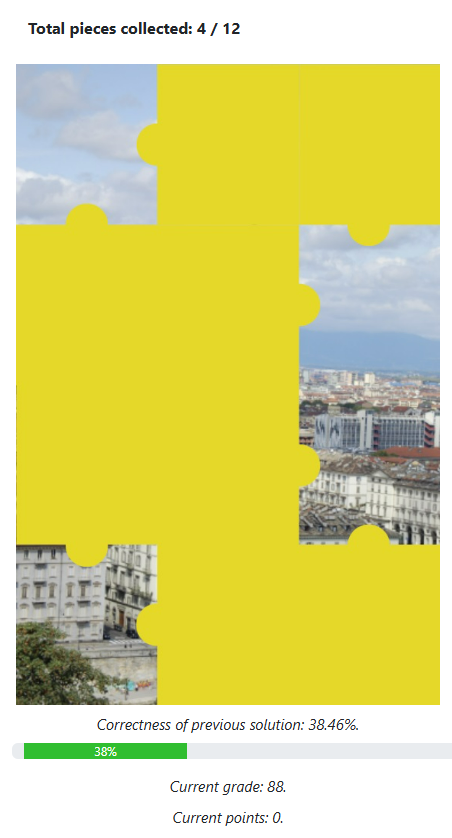
\includegraphics[width=0.5\linewidth]{Template_Latex_ScuDo_Tesi//Chapter3/sidebar.png}
        \caption{Exercise page sidebar implementing the \textit{Rewards}, \textit{Progress}, and \textit{Penalty} mechanics}
        \label{fig:sidebar}
    \end{figure}
    \item The \textit{Progress} concept was kept as a progress bar displayed in the exercise's user interface that updated depending on the results of an evaluation. The bar would originally be empty when starting an exercise and would update after every check activated by a student, reporting the completeness percentage of the exercise as the number of correctly modeled part (that is, parts with matching elements) over the total number of parts that compose the exercise. An example of what the progress bar looks like can be seen in Figure \ref{fig:sidebar}.
    \item In line with how it was decided to structure the simulated experience, the \textit{Penalty} mechanic was implemented in the form of the grade assigned to the exercise: any time a student uses the evaluation engine to check the correctness of their solution, the grade gets reduced by a value tied to the number of process parts that do not have matching elements in the diagram. The grade reduction is applied after every check, to deter students from submitting the same diagram over and over with no changes. This mechanic mirrors the points that can be traded for puzzle pieces, as the reduction for non-modeled parts is the same as the number of points that are obtained for including a process part (meaning that less complex part reduce the grade less compared to more detailed ones). Figure \ref{fig:sidebar} shows the indication of the current grade's value in the application sidebar.
    \item The \textit{Feedback} mechanic was implemented in two steps: first of all, a dedicated modal window is displayed after every automated evaluation, displaying the list of parts that are not represented, as well as those that have matching diagram elements, with the number of points that have been deducted from the grade or obtained, respectively, as displayed in Figure \ref{fig:feedback_modal}. 
    \begin{figure}
        \centering
        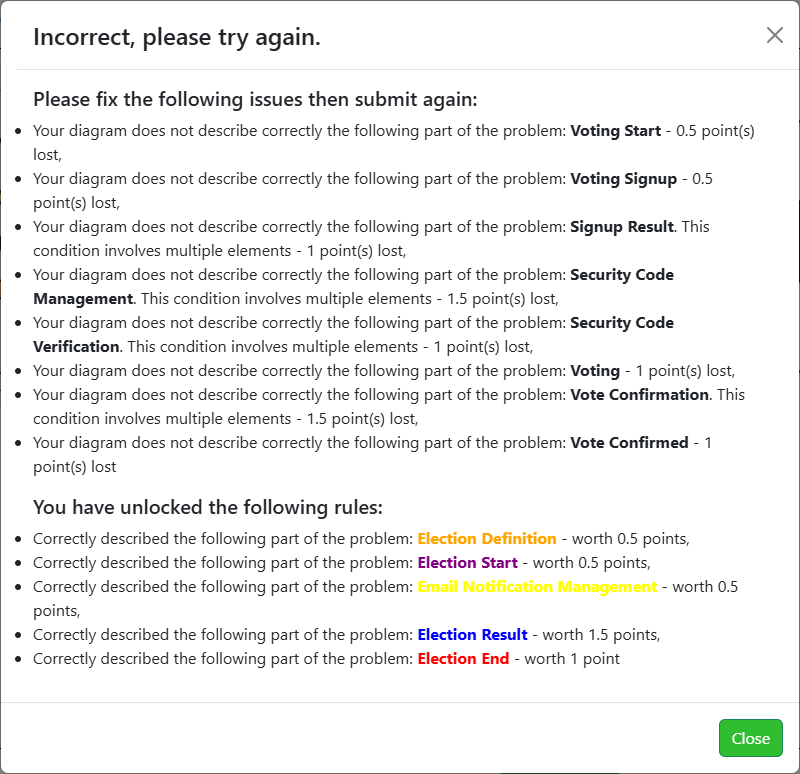
\includegraphics[width=0.6\linewidth]{Template_Latex_ScuDo_Tesi//Chapter3/feedback_modal.png}
        \caption{Modal window shown after an automated evaluation listing which process parts are modeled and which ones are still missing}
        \label{fig:feedback_modal}
    \end{figure}
    Moreover, each process part has an associated color, which is used when presenting the parts that have been modeled correctly in the modal window; the main purpose of the color, however, is to change the background of the elements that have been considered matching for the process parts in the same way, highlighting which parts of the student's diagram are considered correct and which ones are not. An example of what the feedback mechanism looks like in practice is shown below, with Figure \ref{fig:clean_diagram} showing a BPMN diagram before an automated evaluation, and Figure \ref{fig:feedback_diagram} showing the same diagram after the automated evaluation, with the colored elements signifying that the upper pool is correctly representing part of the requirements, while the lower one needs to be improved.
    \begin{figure}[H]
    \centering
    \begin{subfigure}{0.48\linewidth}
        \centering
        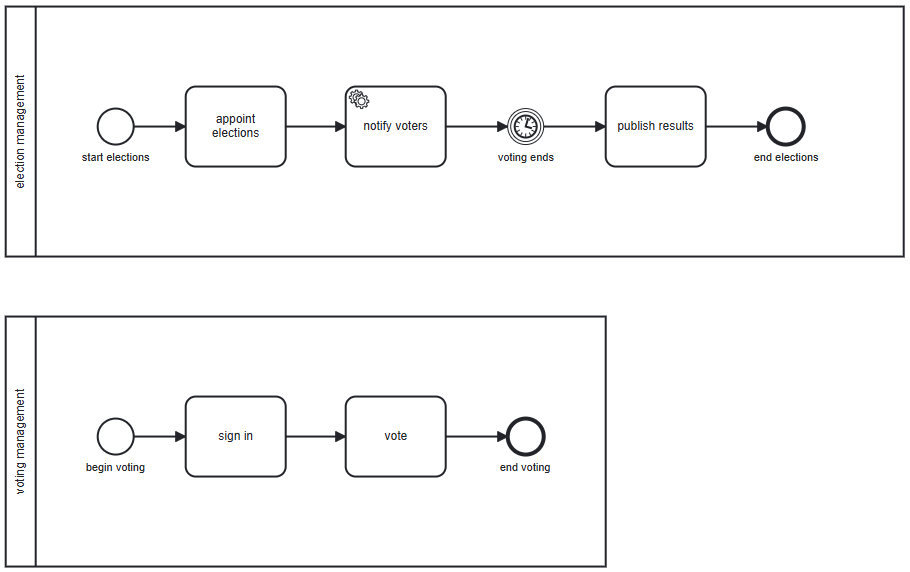
\includegraphics[width=\linewidth]{Template_Latex_ScuDo_Tesi/Chapter3/clean_diagram.png}
        \caption{BPMN diagram not yet submitted to an automated evaluation}
        \label{fig:clean_diagram}
    \end{subfigure}\hfill
    \begin{subfigure}{0.48\linewidth}
        \centering
        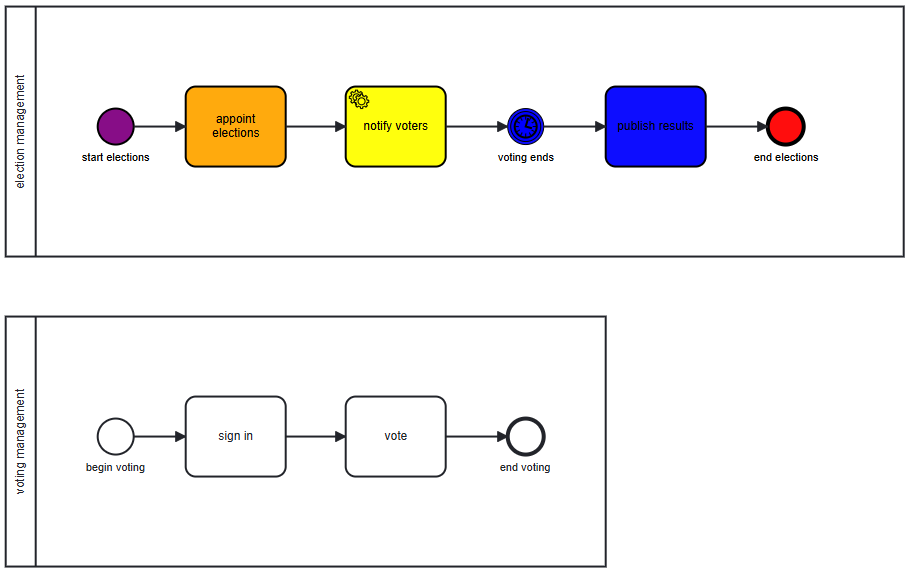
\includegraphics[width=\linewidth]{Template_Latex_ScuDo_Tesi/Chapter3/feedback_diagram.png}
        \caption{BPMN diagram with changes applied after an automated evaluation and coloring for elements that satisfy conditions for certain process parts}
        \label{fig:feedback_diagram}
    \end{subfigure}
    \caption{Implementation of the \textit{Feedback} mechanic via the changes to a student's diagram}
    \label{fig:feedback_example}
    \end{figure}
\end{itemize}


\subsection{Empirical experiment on the improved prototype}

After the implementation of the improved evaluation engine, and the refactoring of game mechanics to be compatible with it, the intended empirical experiment was planned for execution in January 2023. The goal of the experiment was to investigate whether gamification could have an impact on learning BPMN modeling practices, leading to an increase of productivity and correctness. For this purpose, the experiment was framed according to the Goal-Question-Metric (GQM) template, with its purpose being expressed as \emph{assess the impact of gamification on the production of BPMN diagrams and their correctness from the point of view of BPMN modeling teachers in the context of university courses}, while the summary of the experiment according to the GQM template is presented in Table \ref{tab:gqm3}.

\begin{table}[ht]
\small
\centering
\caption{GQM Template for the empirical experiment on the improved BIPMIN}
\begin{tabular}{@{}p{0.3\columnwidth} p{0.55\columnwidth}@{}}
\toprule
Object of Study & BPMN modeling education\\ 
Purpose & Compare the traditional and gamified approach \\
Focus & Productivity, Correctness \\
Context & University modeling courses, modeling tools \\
Perspective & Researchers, teachers \\ \bottomrule
\end{tabular}
\label{tab:gqm3}
\end{table}

\subsubsection{Study Design and participants}

Participants were recruited for the experiment via convenience sampling among the students enrolled in the \textit{Information Systems} course offered by the Masters' level in Management Engineering at Politecnico di Torino. Participants were selected via voluntary participation, which was awarded with 2 additional points out of the 30 assigned to the course's final exam grade; furthermore, students were reassured that participation was optional since the beginning of the course, and that there would have been no negative consequences for not attending the experiment, nor for performing sub-optimally during the experiment itself. The resulting cohort of participants was a total of 200 students, with 95 female students and 105 male ones. The experiment was conducted in a mixed way: to account for the students' availability, it was possible to participate either in person at Politecnico di Torino's computer laboratories or remotely with one's personal device; for students participating remotely, an online chat room was set up to provide assistance during the study, ensuring that instructions and general feedback were available for all participants involved.

Since the study focused on the impact of gamification on BPMN modeling practices, the experimental design needed to introduce a way for participants to compare regular BPMN modeling with the enhancements brought by BIPMIN. For this reason, the within-subjects design was selected once again, meaning that participants would have to execute modeling tasks both with and without gamification. The participants were recruited from the students of a course where BPMN is taught as a topic with both theory lectures and practical laboratory sessions where students complete modeling assignments on their own using an online platform called Signavio Academic; this platform offers a way for its users to check if a BPMN diagram contains BPMN syntax violations, in a way that is similar to what the \textit{bpmnlint.js} library implemented in BIPMIN allows to do, meaning that students were already used to modeling with syntactic assessment.

To ensure fairness in the comparison between the presence of the treatment (gamification) or not, it was decided that students would not use Signavio for the non-gamified task: a modified version of BIPMIN with no gamified mechanics was developed instead; this version offered the basic syntax evaluation features, to be in line with what the students were using during the course. The two treatments were thus finalized according to the version in use, with the original BIPMIN representing the \textbf{Gamified} version and the non-gamified version with simple syntax checking being named the \textbf{Vanilla} version.

After settling on the experiment design and how to administer the treatment, the number of tasks was finalized as a total of two exercises, one per each treatment: this resulted in a 2x2 full factorial crossover experiment where, depending on the combination of both the treatment (Gamified-then-Vanilla or Vanilla-then-Gamified) and task (Exercise 1 followed by Exercise 2 or vice-versa), a total of four possible experimental conditions could be possible; the four possible combinations defined four possible groups and are presented in Table \ref{tab:exp_design_3}. To ensure fairness, participants were randomly assigned to the four groups, ensuring that each group had a total of 50 participants.


\begin{table}[H]
\centering
\footnotesize
\caption{Experiment Design}
\label{tab:exp_design_3}
\resizebox{\textwidth}{!}{%
\begin{tabular}{l c c c c}
\toprule
& \multicolumn{2}{c}{Task 1} & \multicolumn{2}{c}{Task 2} \\
& Exercise & Tool & Exercise & Tool \\
\midrule
Group 1 & Exercise 1 & Vanilla & Exercise 2 & Gamified \\
Group 2 & Exercise 1 & Gamified & Exercise 2 & Vanilla \\
Group 3 & Exercise 2 & Vanilla & Exercise 1 & Gamified \\
Group 4 & Exercise 2 & Gamified & Exercise 1 & Vanilla \\
\bottomrule
\end{tabular}%
}
\end{table}

The two exercises were selected among the exercises defined by the course's supervisors for the exam calls in years before 2023, and consist of the description of real-life scenarios where an Information System is used to facilitate a process involving multiple actors and activities. The exercises were judged by the supervisors to be of average difficulty, and thus suitable for students to solve during the experiment. The experiment was performed at the end of the course, a few weeks before the final exam, and it was assumed that students had the necessary knowledge and preparation to solve the two exercises in a reasonable amount of time: a time constraint was then enforced during the experiment, as participants were imposed a time limit of 45 minutes for each of the two exercises they had to solve.
%The full text of the two exercises is reported in Appendix \ref{app:exercises}, \RO{and examples of solutions accepted by the evaluation engine are available as an online resource\footnote{\url{https://doi.org/10.6084/m9.figshare.22811123.v3}}.} \ROremoved{while Appendixes E and F show examples of solutions accepted by the evaluation engine.} 

Additionally, after the participants had completed the two exercises, a questionnaire was administered to collect their opinion about the overall experience with BIPMIN: this questionnaire included the GAMEX questionnaire, a survey used to measure user perception when using gamified environments, as well as questions that measured the participants' opinions about the game mechanics.

\begin{comment}

We also analyzed the participants' skills in BPMN modeling by observing the sum of the grade assigned to BPMN-related exercises in the course's written exam (up to eight points) with the grade assigned to the BPMN exercise of an optional course assignment (up to two points). 
Results, which are reported in Figure  \ref{fig:grades}, show that most students are fairly skilled in BPMN modeling, with the mean value being 7 points out of 10 total.

\begin{figure}[t]
\includegraphics[width=\columnwidth]{Fig6.eps}
\centering
\caption{Distribution of points for BPMN tasks in exams}
\label{fig:grades}
\end{figure}

For the experiment, we developed a React-based web application, of which we provide a replication package as a Docker container available online\footnote{\url{https://hub.docker.com/r/giacomogaraccione/bipmin}}; additionally, we provide the data analyzed in the experiment (diagrams produced by students, results of the evaluations, answers to the questionnaire) as an online resource\footnote{\url{https://doi.org/10.6084/m9.figshare.24893601.v2}}. 


\end{comment}

\subsubsection{Research Questions and Metrics}

The experiment was designed so that it could provide answers to the following research questions:
\begin{itemize}
    \item \textbf{RQ1:} Does gamification improve the students' \textit{productivity} in modeling BPMN diagrams compared to non-gamified BPMN modeling?\\
    \emph{The intent of this question is to measure whether gamification can make BPMN modeling more appealing, leading to them making more evaluations and control the size of their diagrams.}\\
    This question is further refined into:
    \begin{itemize}
        \item \textbf{RQ1.1:} Does the application of gamification impact the \textit{Size} of the diagrams produced by the students?
        \item \textbf{RQ1.2:} Does the application of gamification impact the \textit{Attempts} made by students?
    \end{itemize}
    \item \textbf{RQ2:} Does gamification improve the \textit{Correctness} of the diagrams modeled by the students compared to non-gamified BPMN modeling?\\
    \emph{The expectation with this question is that gamification can provide a more engaging environment and its mechanic can lead students to produce more correct diagrams.}\\
    This question is further refined into:
    \begin{itemize}
        \item \textbf{RQ2.1:} Does the application of gamification impact the \textit{Syntactic correctness} of the diagrams produced by the students?
        \item \textbf{RQ2.2:} Does the application of gamification impact the \textit{Semantic correctness} of the diagrams produced by the students?
    \end{itemize}
    \item \textbf{RQ3:} What is the students' \textit{Perception} of gamified BPMN modeling?\\
    \emph{The goal of this question is to measure how students perceive gamification.}
    \item \textbf{RQ4:} Does gamification improve \textit{enjoyment} and \textit{perceived usefulness} compared to non-gamified BPMN modeling?\\
    \emph{The assumption behind this question is that students see gamification in a favorable way.}\\
    This question is further refined into:
    \begin{itemize}
        \item \textbf{RQ4.1:} How do students feel about the implemented \textit{Game Mechanics}?
        \item \textbf{RQ4.2:} What are the \textit{Issues} the students found with BIPMIN?
        \item \textbf{RQ4.3:} What are the possible \textit{Improvement areas} for the tool according to the students?
    \end{itemize}
\end{itemize}


The design of the experiment depends on three independent variables, with the treatment being the application of gamification or not, and two other independent variables being the two exercises being used as the experiment tasks and the order in which the treatments are applied. Dependent variables, instead, relate to the potential benefits that gamification could bring when applied to BPMN modeling in terms of student productivity and diagram correctness. Furthermore, the post-experiment questionnaire is used to measure the student's perception of the gamified experience (with the GAMEX constructs), the enjoyment and perception of the game mechanics, and the students' opinions collected with open-ended questions.

The collection of experiment results was performed in two separate ways depending on the source of related data: for metrics related to research questions RQ1 and RQ2, which focus on the diagrams produced by their students and the corresponding feedback produced by the evaluation engine, data was collected automatically by BIPMIN, which saves the students' diagram after each evaluation, keeping for each account and exercise the history of the five most recent evaluations and the corresponding feedback; the diagram and feedback that was last saved at the end of each modeling task were selected as data for analysis.
Regarding the metrics for RQ3 and RQ4, the survey was offered online as a Google Form, which automatically collects all given answers in a single spreadsheet.

The metrics under analysis have been distinguished according to the different research questions: regarding RQ1, \textit{Productivity} was measured with the \textit{Size} of diagrams, computed as the count of all elements in the diagram, and the \textit{Attempts} made by students, counted as the number of times each student had their solution assessed by the automated evaluator. This metric was further divided into syntax checks, existing in both the non-gamified and gamified versions, and correctness checks focused on semantic quality available only in the gamified version, and only after a diagram was found to have no syntax errors with the first check.

Size was selected as a metric with the assumption that, since the reference solutions were defined with a necessary minimum set of elements for a diagram to be evaluated as correct, there was not going to be high variability in terms of the number of elements that could have been included in the students' diagrams. Additionally, solutions did not cover alternative ways to represent the same process part, with the only variation allowed being in the labels assigned to the elements by allowing synonyms. This way, with a fixed number of required elements for a diagram to be considered correct, it was decided that producing diagrams with more elements equated to being more productive, and that by not allowing variations in the allowed types of elements the risk of considering wrong a diagram that was actually correct was reduced.

As for answering RQ2, \textit{Correctness} was split into \textit{Syntax correctness} and \textit{Semantic correctness}. The former was measured as the percentage of syntax rules satisfied by a diagram over the total number of syntax rules, while the latter was computed as the number of process parts modeled by a diagram over the total number of parts. This metric represents diagram correctness, and should not be confused with the semantic error count metric used in Chapters \ref{ch4} and \ref{ch5}, a metric that measures incorrect domain representation choices.

RQ3 related to the students' perception of the gamified experience, which was assessed with the GAMEX questionnaire described in Section \ref{sec:empirical_methods}, using a Likert scale ranging from 1 - \textit{Strongly Disagree} to 5 - \textit{Strongly Agree} to express the answers %The full list of questions is visible in Tables \ref{tab:q12}, \ref{tab:q34}, and \ref{tab:q56} of Appendix \ref{app:questionnaire}.

To answer RQ4, the questionnaire included questions about the four game mechanics implemented in BIPMIN: more precisely, three questions were included for each mechanic, asking the participants how the mechanic had influenced their experience, whether they thought the mechanic was useful, and how much they had appreciated the mechanic. Answers to these questions were also expressed as Likert scale questions, with the same range as the GAMEX questions. Furthermore, the questionnaire included two open-ended questions: the first one asked participants to describe any issues they had experienced during the study, while the second asked them to report comments and opinions that they believed could help improve the overall experience. %Appendix \ref{app:questionnaire} lists the questions related to the gamified mechanics in Table  \ref{tab:game_questions}: those questions allowed answers in the form of Likert-scale values, using the same range used for RQ3. The two open questions are also included in the same Appendix.

\subsubsection{Analysis Method}

To answer RQ1 and RQ2, null hypotheses have been formulated around the metrics discussed above. These hypotheses are presented as follows:

\begin{itemize}
    \item ${H_{s_{0}}}$: Gamification has no statistically significant impact on the \textit{Size} of the diagrams submitted by students
    \item ${H_{as_{0}}}$: Gamification has no statistically significant impact on the \textit{Attempts} made by students
    \item ${H_{syc_{0}}}$: Gamification has no statistically significant impact on the \textit{Syntax Correctness} of the diagrams submitted by students
    \item ${H_{sec_{0}}}$: Gamification has no statistically significant impact on the \textit{Semantic Correctness} of the diagrams submitted by students
\end{itemize}

Given that the experiment was designed as a full factorial crossover study, the data was analyzed using a repeated measures linear mixed models, according to the guidelines by Vegas et al. \cite{vegas2016crossover}; furthermore, the two exercises and the order of treatment have also been considered design factors during the analysis, to counteract possible threats to validity related to the design.

RQ3 and RQ4, instead, were evaluated through a questionnaire whose answers could not be analyzed with statistical hypothesis testing; the answers were analyzed through descriptive statistics, with a focus on the distribution of scores for Likert-scale questions (RQ3 and RQ4.1). For these questions, the analysis method consisted of computing the average score assigned to each set of questions as the overall opinion for each student, and then plotting the distribution. Lastly, RQ4.2 and RQ4.3 were answered with open-ended questions where students could present their opinions: these answers were analyzed using the open coding strategy from Straussian Grounded Theory (see Section \ref{sec:empirical_methods}) \cite{strauss1998basics}. Each answer was labeled with the most compatible topic from a growing set, with two subsequent passes to refine assignments and identify answers for which multiple topics were suitable.

\subsubsection{Results}

Table \ref{tab:m1stats} lists summary statistics about the metrics selected for answering RQ1, that is, the minimum, maximum, mean, median, and standard deviation of the diagram size of each student's final saved diagram, as well as the number of attempts made by students, computed as the number of evaluation checks performed during each task; these metrics are grouped depending on the exercise first, then on the treatment, and then over both exercises depending on the treatment (with or without gamification). The distributions of the two metrics over the two exercises depending on the application of gamification or not have been represented in a combined box and violin plot, and can be seen in Figure \ref{fig:m1boxplots}.

\begin{table}[ht]
  \centering
  \small
  \caption{Summary statistics for \textit{Productivity} metrics}
  \label{tab:m1stats}
  \resizebox{\columnwidth}{!}{%
  \begin{tabular}{llcccccc}
    \toprule
    & & \multicolumn{2}{c}{Exercise 1} & \multicolumn{2}{c}{Exercise 2} & \multicolumn{2}{c}{Total} \\
    & & \multicolumn{1}{c}{V} & \multicolumn{1}{c}{G} & \multicolumn{1}{c}{V} & \multicolumn{1}{c}{G} & \multicolumn{1}{c}{V} & \multicolumn{1}{c}{G} \\
    \midrule
    Size & Min & 19 & 27 & 25 & 27 & 19 & 27 \\
    & Max & 119 & 93 & 78 & 79 & 119 & 93 \\
    & Mean (SD) & 61.7 (13.3) & 61.2 (12.3) & 48.6 (10.6) & 50.5 (10.6) & 55.1 (13.7) & 55.9 (12.7) \\
    & Median & 60.0 & 60.0 & 48.5 & 50.5 & 54.0 & 56.0 \\
    \midrule
    Attempts & Min & 1 & 1 & 1 & 1 & 1 & 1 \\
    & Max & 25 & 61 & 17 & 55 & 25 & 61 \\
    & Mean (SD) & 6.5 (4.28) & 14.6 (10.9) & 5.7 (3.37) & 14.5 (10.07) & 6.1 (3.86) & 14.5 (10.47) \\
    & Median & 6.0 & 11.5 & 5.0 & 12.0 & 5.0 & 12.0 \\
    \bottomrule
  \end{tabular}%
  }
\end{table}

\begin{figure}[H]
    \centering
    \begin{subfigure}{0.7\linewidth}
        \centering
        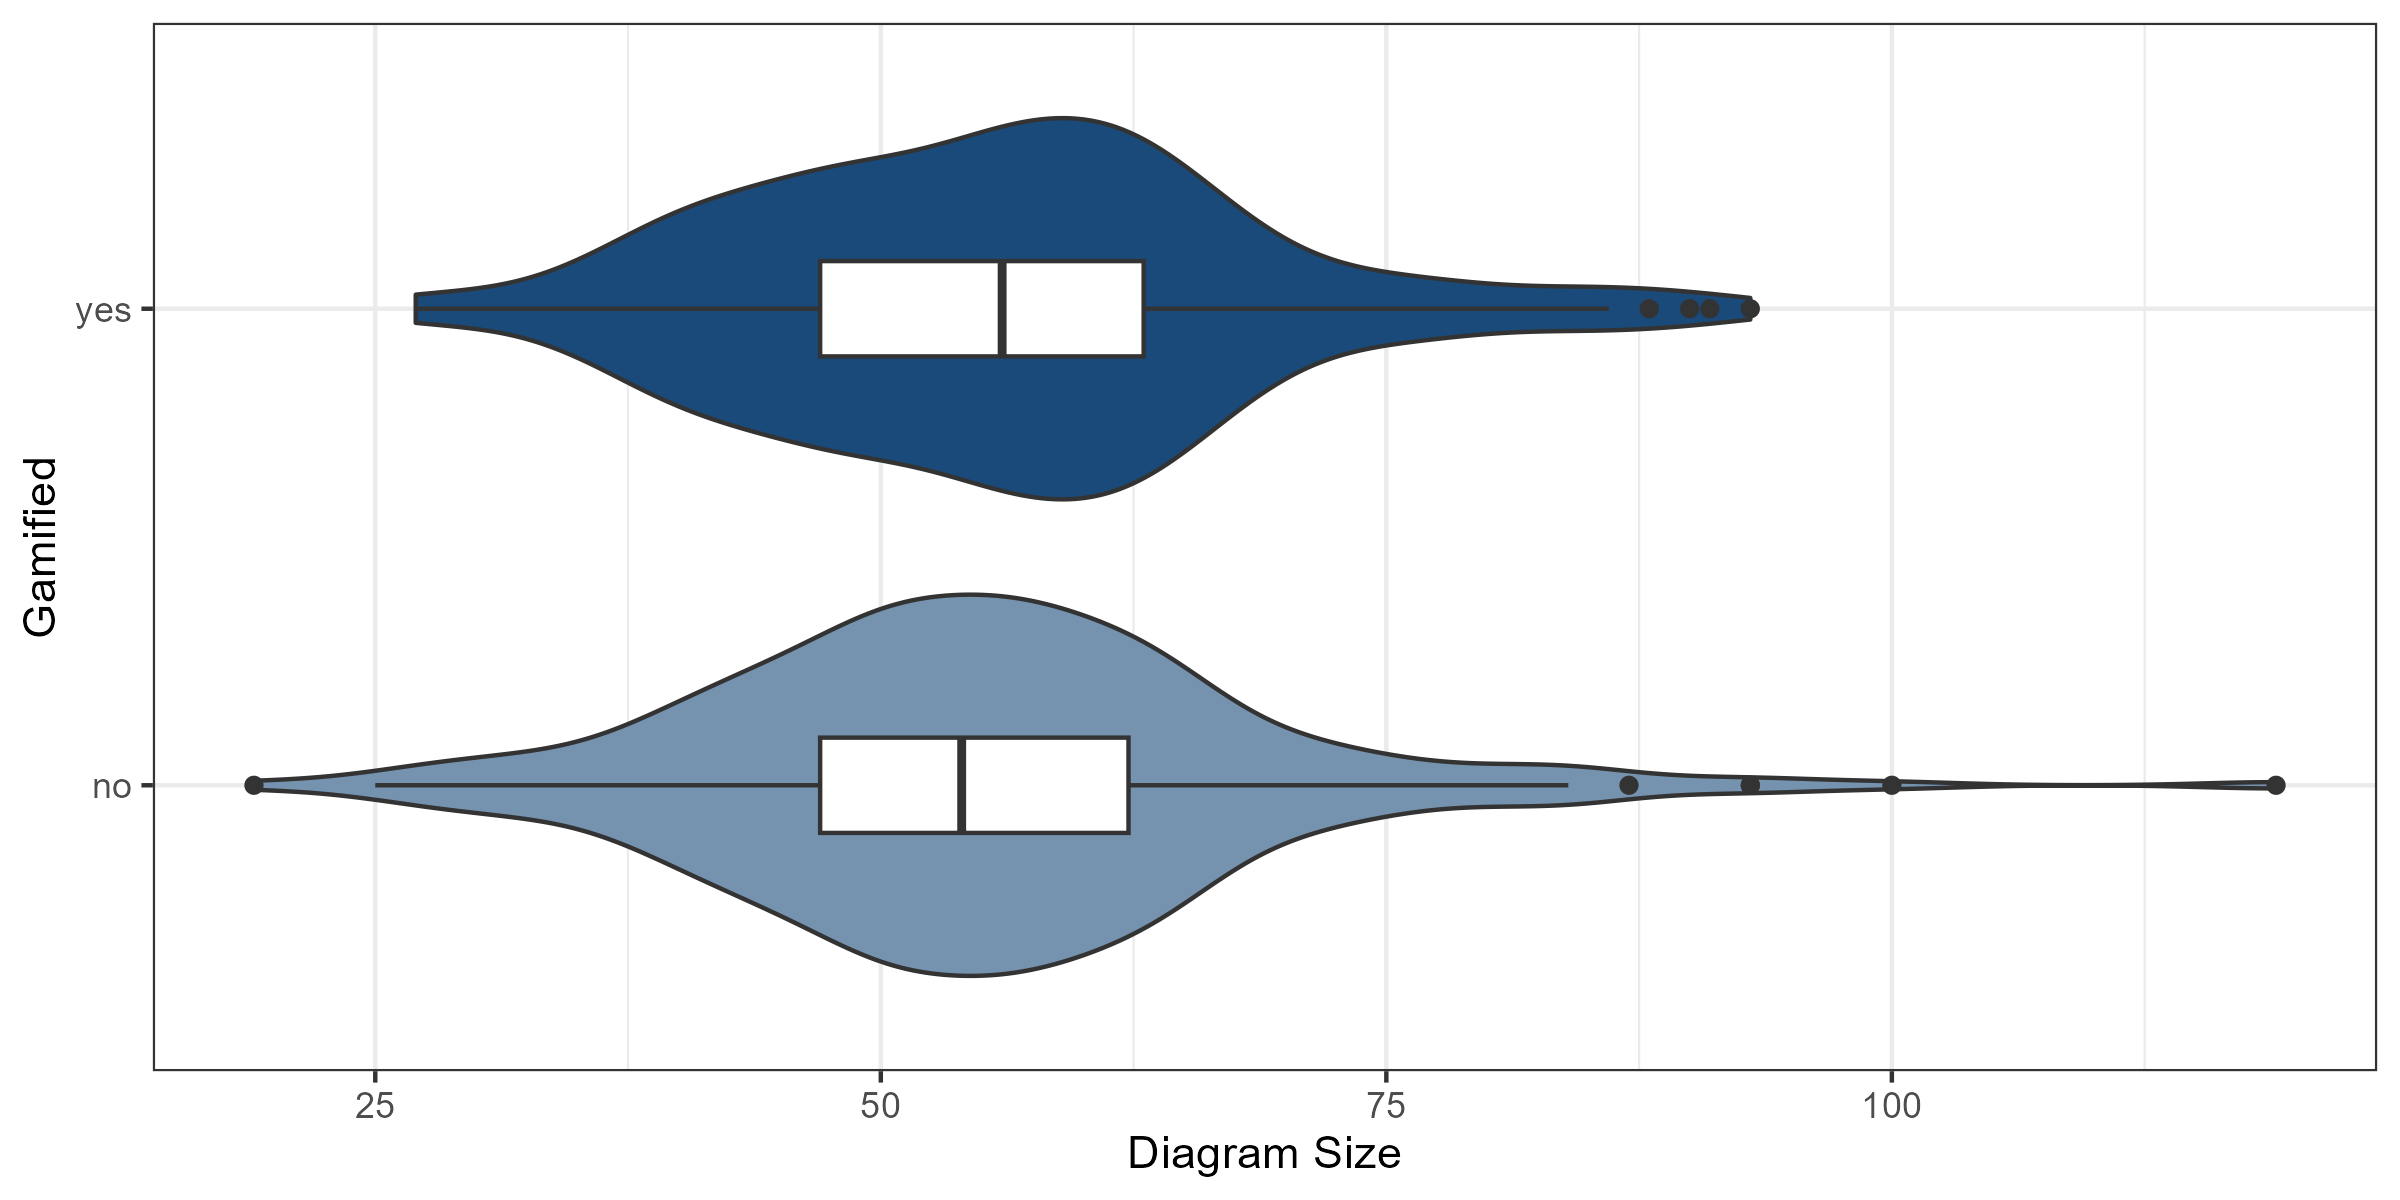
\includegraphics[width=\linewidth]{Template_Latex_ScuDo_Tesi/Chapter3/exp_size_violin.png}
        \caption{Box and violin plot for the \textit{Size} metric}
        \label{fig:boxplotsize}
    \end{subfigure}\hfill
    \begin{subfigure}{0.7\linewidth}
        \centering
        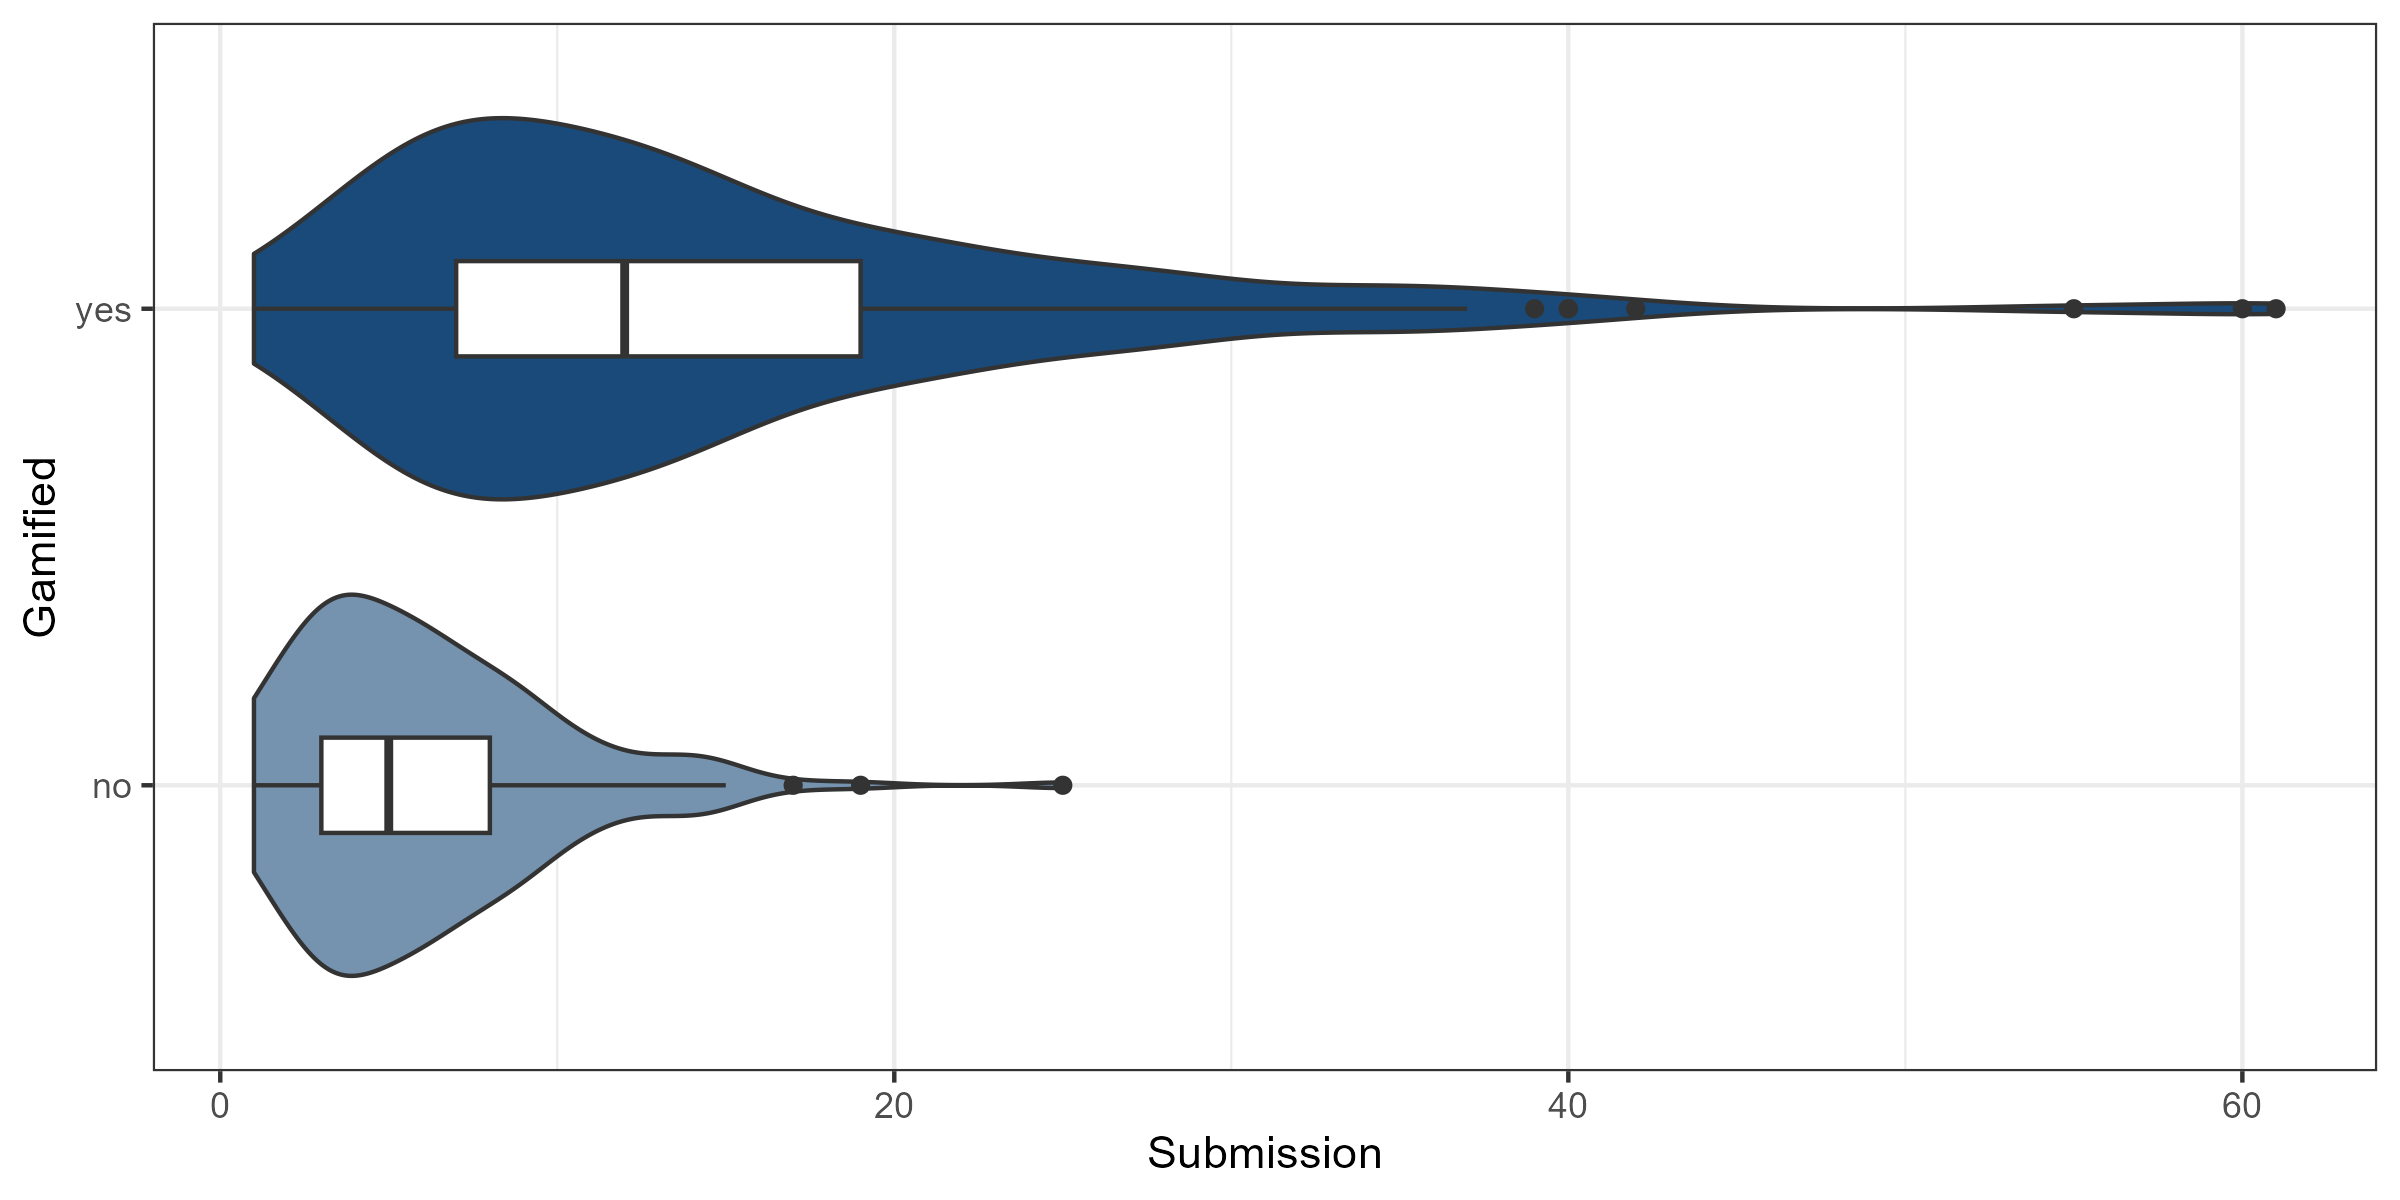
\includegraphics[width=\linewidth]{Template_Latex_ScuDo_Tesi/Chapter3/exp_subs_violin.png}
        \caption{Box and violin plot for the \textit{Attempts} metric}
        \label{fig:boxplotsubs}
    \end{subfigure}
    \caption{Box and violin plots for RQ1 metrics}
    \label{fig:m1boxplots}
\end{figure}

When considering the \textit{Size} metric, it can be seen immediately that, on average, there are no differences when it comes to the treatment, meaning that this value remains almost identical (55.1 elements to 55.9), with a minor increase for the gamification version. When comparing the combination of treatment and task, that is, use of gamification and exercise to solve, a similar result is obtained for the first exercise, where the average size is almost identical both with and without gamification; the second exercise, instead, has a slight difference, with diagrams produced with gamification having a slightly higher average size (50.5 against 48.6). It could be assumed that, on average, applying gamification to BPMN modeling exercises does not lead students to make substantial changes to their diagrams by adding or removing elements.

Some differences can actually be observed with regards to the \textit{Attempts} metric, since there is a much higher average number of solution checks made by students when using the gamified version, considering both exercises and considering the overall distribution of these attempts: the immediate interpretation of this result is that the implemented game mechanics lead students to perform more evaluations of their diagrams, since the results of an evaluation impact the four game mechanics.

To answer RQ1, two null hypotheses have been defined, and a repeated measures linear mixed models has been used to analyze the distribution of diagram size and evaluation attempts: Table \ref{tab:tabrq1_anova} lists the results of the statistical analysis, showing the difference in average metric scores depending on the use of gamification (Treatment), the task attempted (Exercise), and on whether gamification was applied in the first or second task.

\begin{table}[ht]
  \centering
  \footnotesize
  \caption{Results of the statistical analysis for RQ1 metrics: Size and Attempts. Statistically significant p-values are in bold}
  \label{tab:tabrq1_anova}
    \begin{tabular}{lcccc}
         \toprule
         Factor / vars:& 
         \multicolumn{2}{c}{Size (${H_{s_{0}}}$)} & \multicolumn{2}{c}{Attempts (${H_{as_{0}}}$)} \\
         & coeff. & p-value & coeff. & p-value \\
         \midrule
         Treatment & -0.3775	& 0.2170 & -4.215 & \textbf{$\lt$ 2e-16} \\
         Exercise & -5.9700 & \textbf{ $\lt$ 2e-16} & -0.2100 & 0.2525\\
         Order & 0.4750 & 0.4230 & -2.2300 &	\textbf{0.0056}\\
         \bottomrule
    \end{tabular}

\end{table}

The results of the statistical analysis focused on the treatment use as reference the non-gamified version: as a consequence, it can be deduced that diagrams produced without gamification tend to have a smaller size and require fewer attempts by students. Furthermore, there is a statistically significant effect on the number of attempts: this, in combination with the resulting coefficient, means that the null hypothesis ${H_{as_{0}}}$ can be rejected, and it can be said gamification leads students to perform more correctness checks on their produced diagram compared to simply allowing for syntactic assessments. The corresponding p-value for the diagram size, however, is not significant: ${H_{s_{0}}}$ cannot be rejected, meaning that gamification does not impact the students' tendency to make significant changes to their diagrams by increasing their element count.

The analysis of confounding factors shows that there is a statistically significant difference in diagram size depending on the exercise: the analysis considered the second exercise as reference, and thus it can be said that it required students fewer elements for them to be satisfied compared to the first, due to the negative value of the coefficient; no significant difference was found for the number of attempts, with a negligible difference between the two exercises. The order of treatment, used the order where gamification was applied in the second task as reference: this yielded no significant result in the diagram size, with a difference of around half an element on average, and a very slightly significant difference in terms of attempts, with the coefficient being negative; the result can be interpreted by assuming that moving from a version with no game elements to one that had them led students to need less checks to be satisfied.

\answer{RQ1}{The use of gamification to enhance BPMN modeling education had no relevant effect on the size of the student-produced diagrams, implying that it does not cause students to make significant changes; it does, however, have a positive effect on the number of attempts, computed as the number of correctness checks performed by the students: by adopting gamification students were more willing to evaluate the correctness of their produced diagrams. Other factors in the experiment's design also had an impact: one exercise required fewer elements to be done by the students, and performing the gamified exercise as the second task made students perform fewer evaluations on their diagram compared to those who had it as the first exercise.}

To answer RQ2, completeness scores have been computed for each saved student diagram as percentages: for syntactic correctness, the score was computed as the number of syntax rules implemented in BIPMIN for which a diagram contained no violations over the total number of syntax rules, while semantic correctness was computed as the number of correctly modeled process parts, according to the predefined reference solutions for the two exercises. Summary statistics for these two variables can be found in Table \ref{tab:m2stats}, which lists them depending on the combination of exercise and treatment, as well as over both exercises depending on whether gamification was used or not; for the latter distribution of scores, a graphical representation is also included in Figure \ref{fig:m2boxplots}.

\begin{table}[ht]
  \centering
  \small
  \caption{Summary statistics for \textit{Correctness} metrics}
  \label{tab:m2stats}
  \resizebox{\columnwidth}{!}{%
  \begin{tabular}{llcccccc}
    \toprule
    & & \multicolumn{2}{c}{Exercise 1} & \multicolumn{2}{c}{Exercise 2} & \multicolumn{2}{c}{Total} \\
    & & \multicolumn{1}{c}{V} & \multicolumn{1}{c}{G} & \multicolumn{1}{c}{V} & \multicolumn{1}{c}{G} & \multicolumn{1}{c}{V} & \multicolumn{1}{c}{G} \\
    \midrule
    Syntactic (\%) & Min & 40 & 43 & 62 & 50 & 40 & 43 \\
    & Max & 100 & 100 & 100 & 100.0 & 100 & 100 \\    
    & Mean (SD) & 90.8 (11.0) & 91.7 (10.5) & 91.4 (9.01) & 92.6 (10.9) & 91.1 (10.0) & 92.2 (10.7) \\
    & Median & 92.0 & 93.5 & 92.0 & 100.0 & 92.0 & 97.0 \\
    \midrule
    Semantic (\%) & Min & 0 & 0 & 0 & 0 & 0 & 0 \\
    & Max & 38 & 85 & 31 & 62 & 38 & 85 \\
    & Mean & 13.2 (11.8) & 19.4 (17.2) & 11.2 (8.8) & 13.0 (10.4) & 12.2 (10.5) & 16.2 (14.6) \\
    & Median & 15.0 & 15.0 & 8.0 & 15.0 & 8.0 & 15.0 \\
    \bottomrule
  \end{tabular}%
  }
\end{table}

\begin{figure}[H]
    \centering
    \begin{subfigure}{0.6\linewidth}
        \centering
        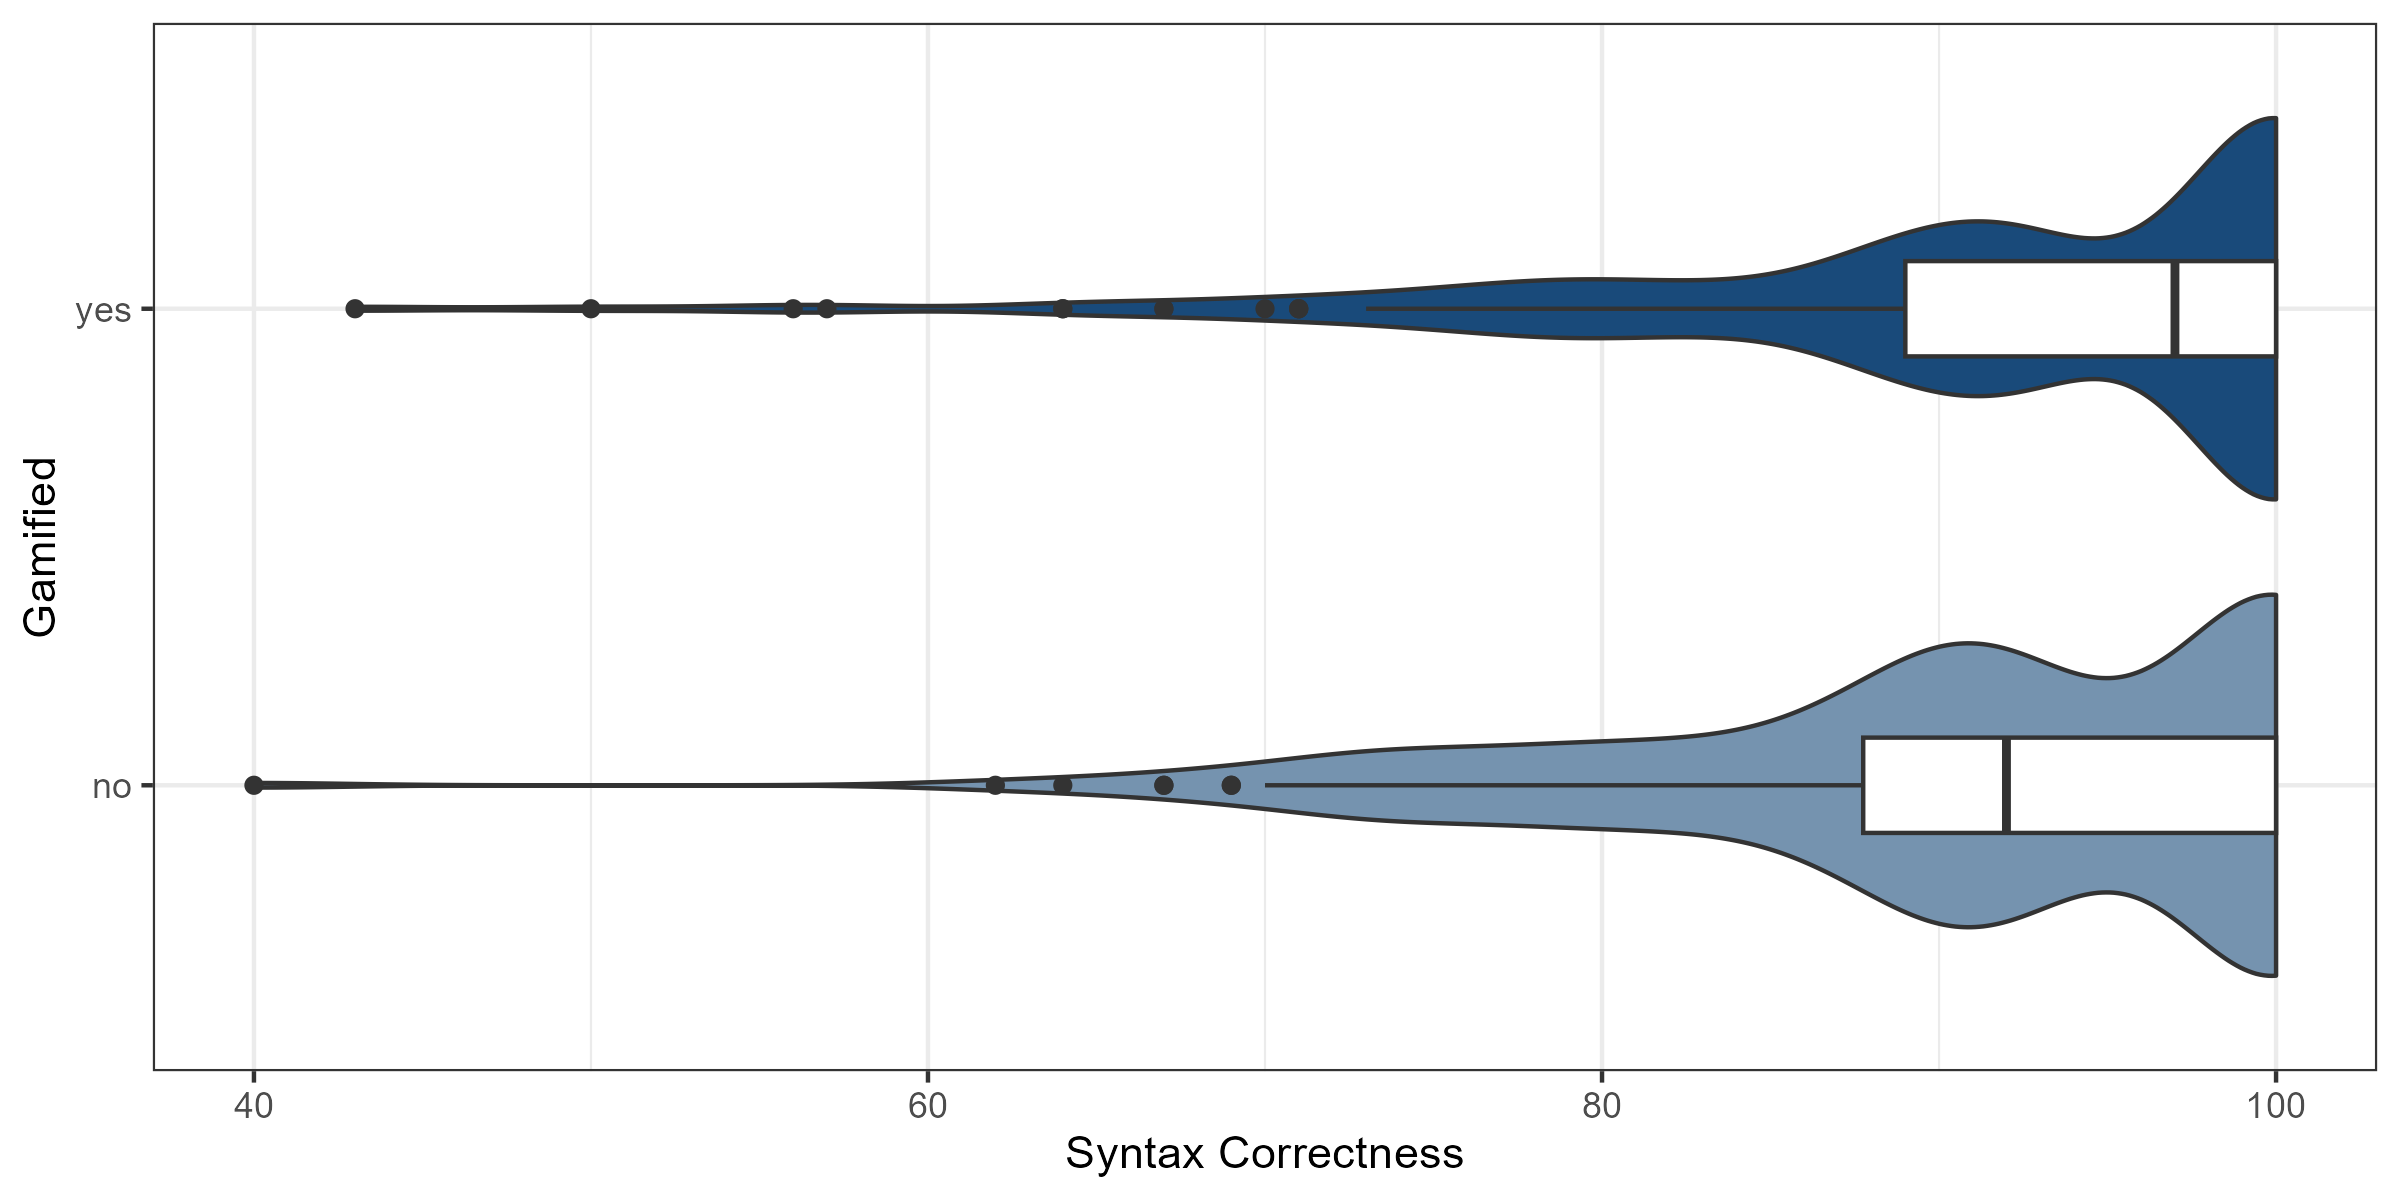
\includegraphics[width=\linewidth]{Template_Latex_ScuDo_Tesi/Chapter3/exp_syn_violin.png}
        \caption{Box and violin plot for the \textit{Syntactic correctness} metric}
        \label{fig:boxplotsyn}
    \end{subfigure}\hfill
    \begin{subfigure}{0.6\linewidth}
        \centering
        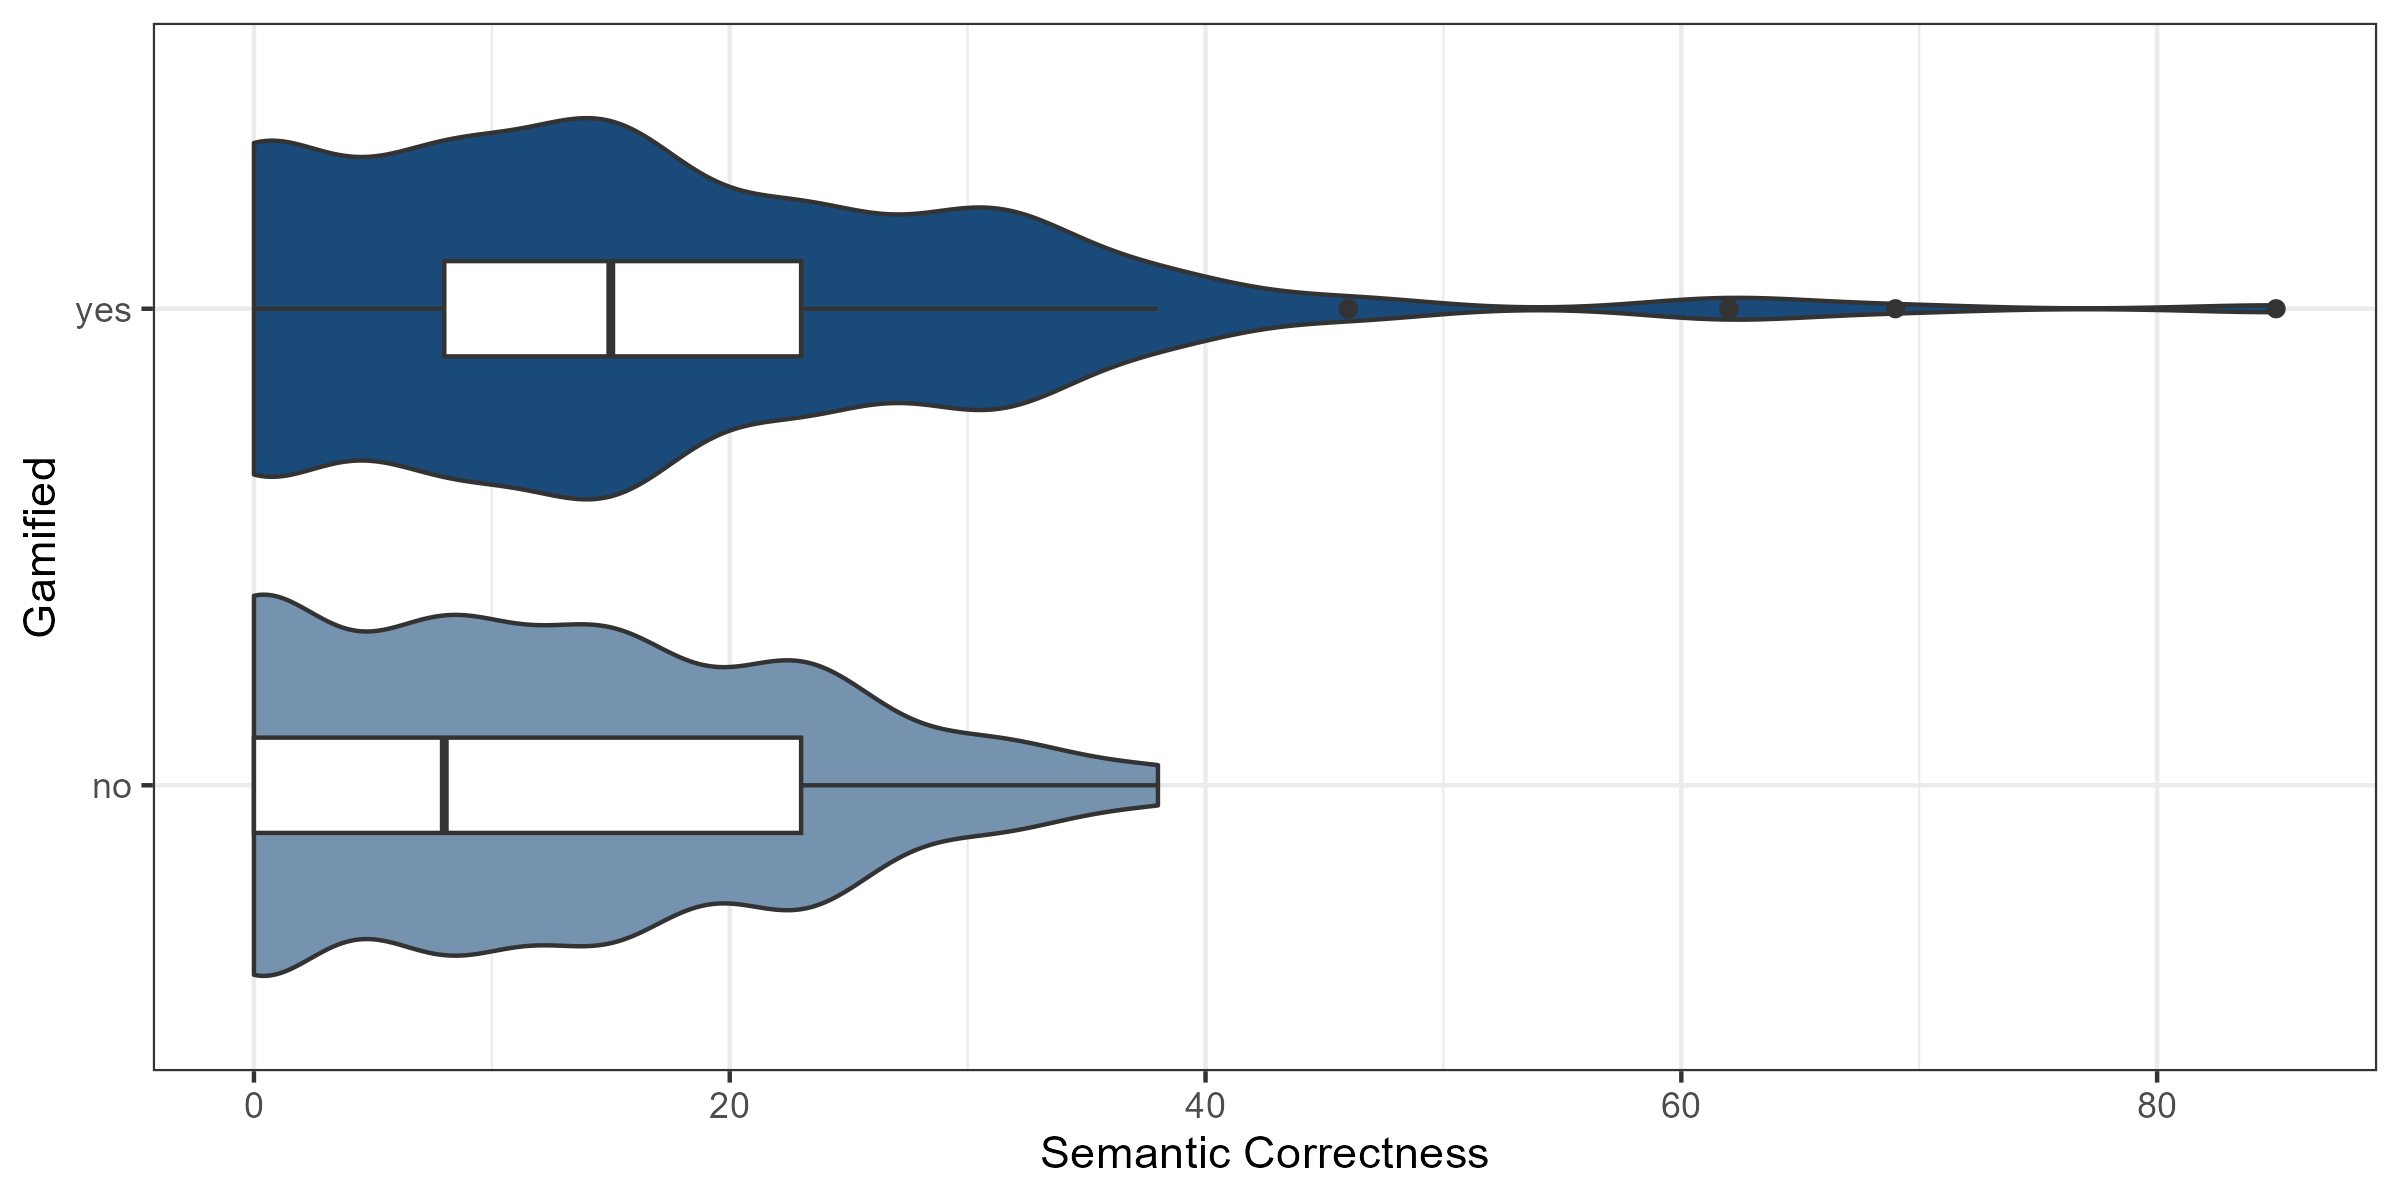
\includegraphics[width=\linewidth]{Template_Latex_ScuDo_Tesi/Chapter3/exp_sem_violin.png}
        \caption{Box and violin plot for the \textit{Semantic correctness} metric}
        \label{fig:boxplotsem}
    \end{subfigure}
    \caption{Box and violin plots for RQ2 metrics}
    \label{fig:m2boxplots}
\end{figure}

Regarding syntactic correctness, it can be seen that the scores are, on average, quite similar between the use of gamification and its absence, implying that the basic implementation of the tool was able to represent an environment similar to the one students were used to, and they were thus able to perform well on said aspects on both versions; no differences can be seen when looking at the combinations of exercise and treatment either, meaning that syntactic performance was similar between the two exercises: it is an expected result, since the two exercises were selected with the assumption that they offered a similar level of difficult and tested similar knowledge requirements, These high scores can also be attributed to the fact that the experiment was performed at the end of the course, and students were consequently more likely to have enough modeling knowledge to avoid syntax errors.

Results related to semantic errors, instead, are slightly more diverse and, unfortunately, do not paint an encouraging picture: the somewhat low mean scores mean that many students performed sub-optimally for the expected preparation level at the end of the course, and it can then be assumed that low performance may depend on the selected exercise or on the effects of BIPMIN itself. The difference in scores between treatments show that the gamified version obtained higher maximum scores, as well as on average, implying that there could have been some benefits brought by gamification.

The results of the statistical analysis focused on RQ2 metrics are presented in Table \ref{tab:tabrq2_anova}: just like for RQ1, results are computed considering the treatment as the factor under analysis and the exercise and order of treatment as possible confounding factors. The analysis considers the non-gamified version as reference for the treatment, and the second exercise and doing the second task with the gamified version as references for the second factor.

\begin{table}[ht]
  \centering
  \footnotesize
  \caption{Results of ANOVA for RQ2 metrics: Syntactical and Semantic Correctness}
  \label{tab:tabrq2_anova}
    \begin{tabular}{lcccc}
         \toprule
         Factor / vars:& 
         \multicolumn{2}{c}{Syntactic (${H_{syc_{0}}}$)} & \multicolumn{2}{c}{Semantic (${H_{sec_{0}}}$)} \\
         & coeff. & p-value & coeff. & p-value \\
         \midrule
         Treatment & -0.5250 &	0.2480 &	-2.0180 & 	\textbf{0.0002}\\
         Exercise & 0.3650 &	1.0000 &	-2.0980 &	\textbf{$\lt$ 2e-16} \\
         Order & -1.7100	& 0.9800 	& -1.0250 &	0.3180 \\
         \bottomrule
    \end{tabular}
\end{table}

The statistical analysis on the treatment shows that, when applying gamification, there is a very slight and non-statistically significant reduction in the syntactic correctness, meaning that ${H_{syc_{0}}}$ cannot be rejected; conversely, the p-value obtained when analyzing the semantic correctness is statistically significant, and ${H_{sec_{0}}}$ can thus be rejected, and it can be said that gamification impacts the semantic correctness of the produced diagrams and, since the negative value of the coefficient implies that the probability of having high semantic correctness is higher when applying gamification, as a consequence, it can be assumed that it can help students better represent and model the required constructs in their exercises.

With respect to confounding factors, no statistically significant difference is found in relation to syntactic quality, strengthening the assumption that, by placing the experiment at the end of the course, students had the sufficient theoretical BPMN knowledge to avoid making syntactic mistakes, and neither the similarly challenging exercises nor moving from regular modeling to gamification enhanced modeling (or vice-versa) impacted their skill. A different result, however, can be found when analyzing results accounting for the exercises: the second exercise yielded a negative coefficient compared to the first and a statistically significant p-value: the first exercise may actually have been slightly easier compared to the second, impacting the overall results. The treatment order had no statistically significant impact on semantic correctness as well, with a very minor reduction in correctness when moving from regular modeling to gamified modeling compared to the opposite order.

\answer{RQ2}{Syntactic correctness was not impacted by any of the factors composing the experiment, due to it being placed at a moment in time when students had sufficient BPMN modeling expertise. Applying gamification had a positive effect on the semantic correctness, however, leading to more correct and complete diagrams in comparison to regular modeling; semantic correctness was also affected by the two selected exercises, with one of them being easier to model than the other.}

To answer RQ3 and RQ4, a post-study questionnaire was given to the participants, aimed at collecting their opinions about the experience and how they had perceived the gamified tool; out of the 200 participants, one of them did not answer, resulting in a total of 199 answers gathered and analyzed.

To answer RQ3, the questionnaire included questions taken from the GAMEX questionnaire, with the sets of questions considered during the analysis being its six constructs; the distribution of answers can be seen in Figure \ref{fig:m3overview}.

\begin{figure}[t]
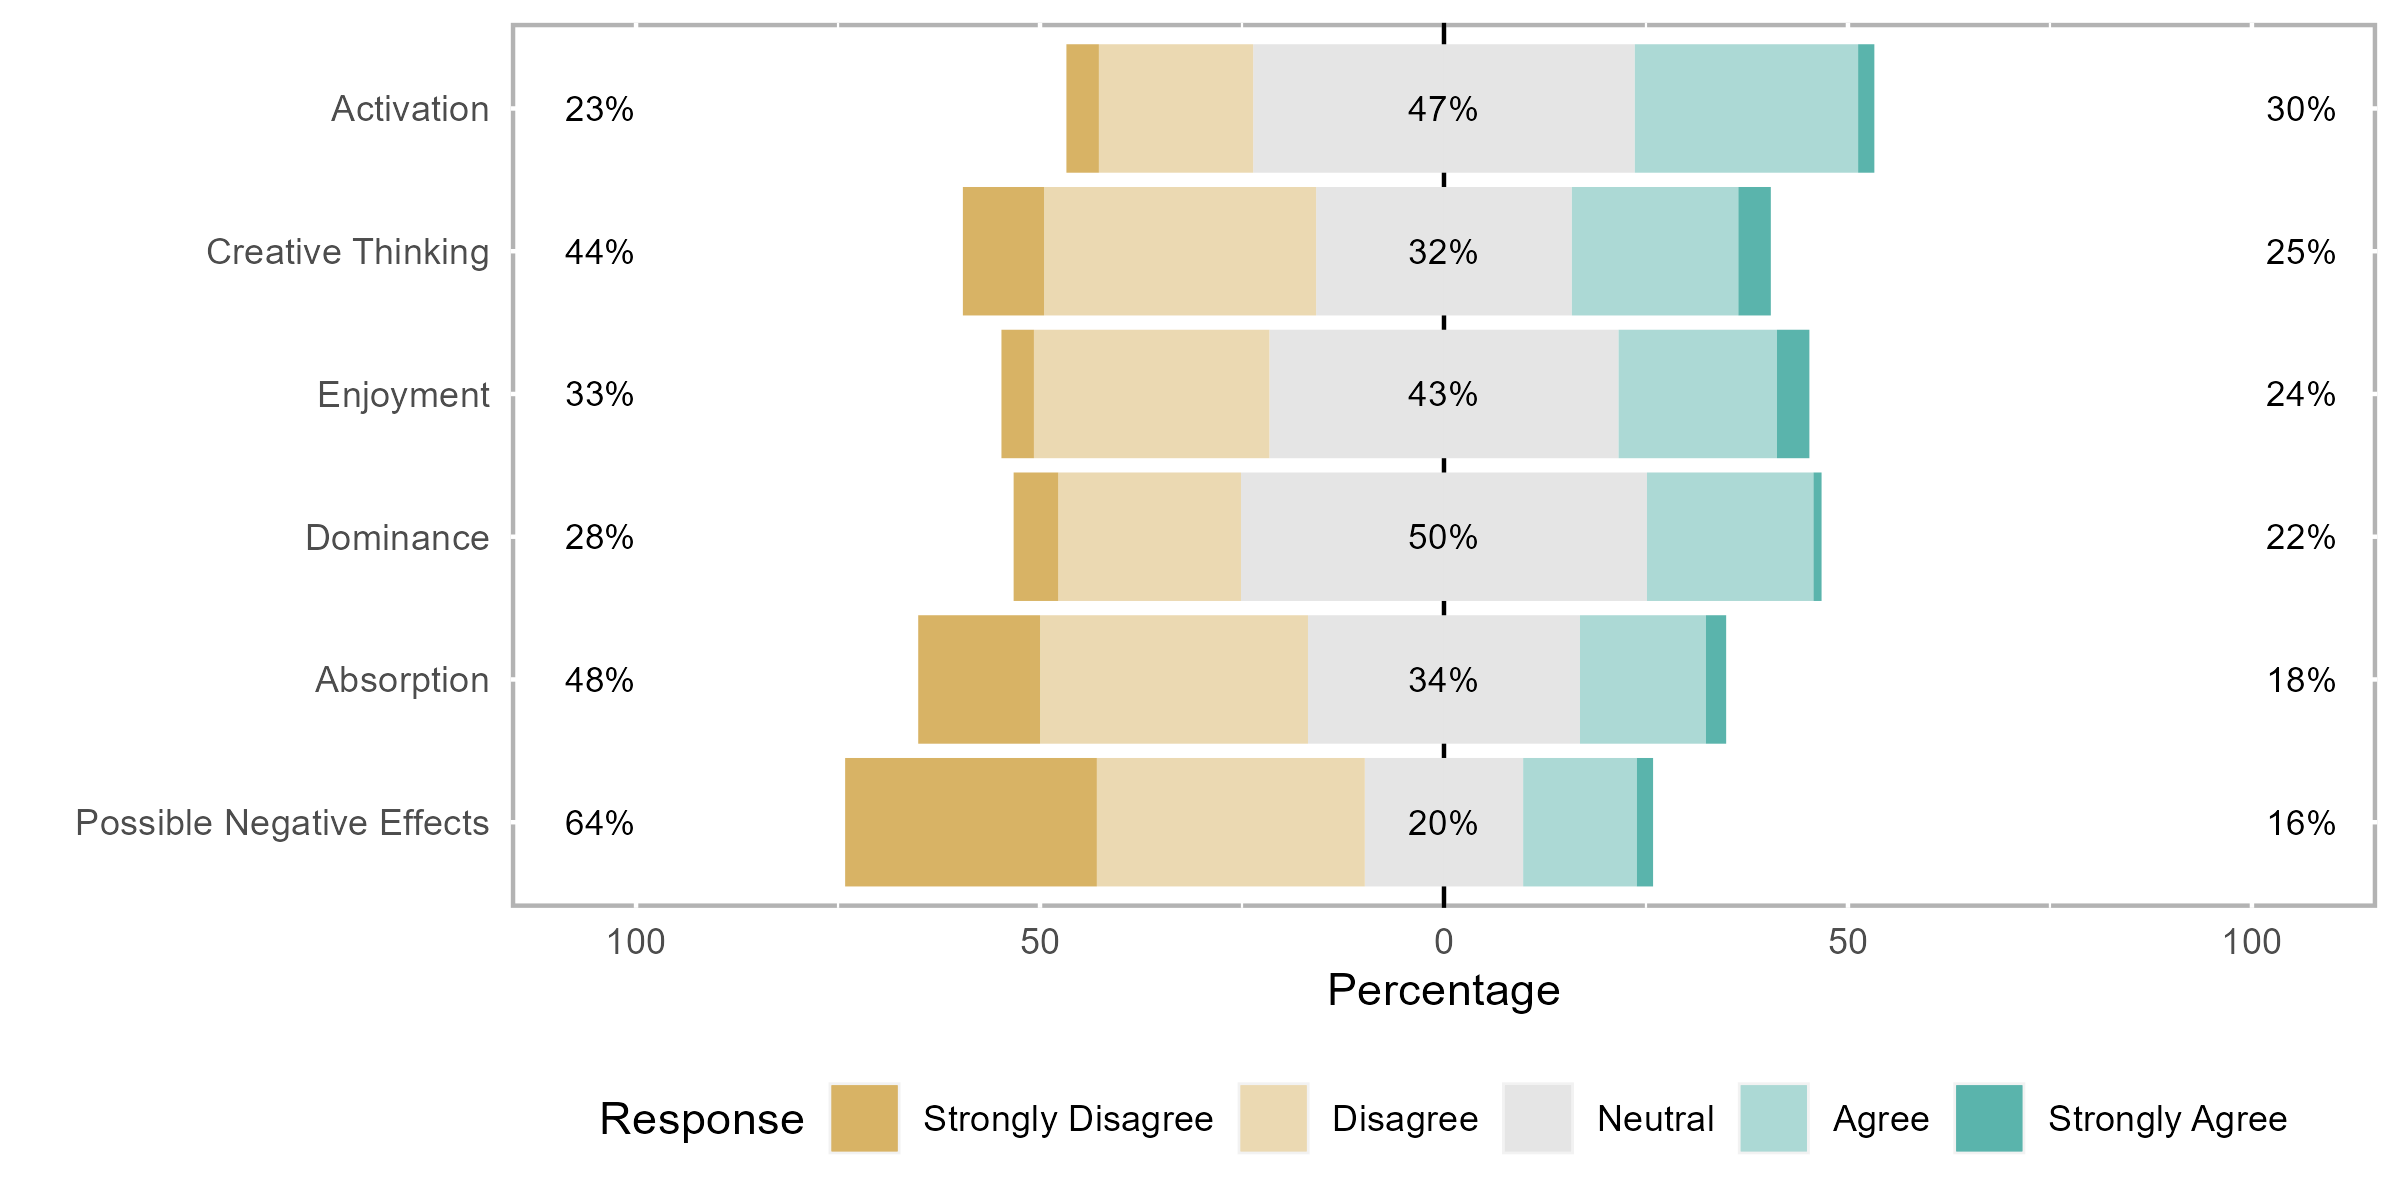
\includegraphics[width=\columnwidth]{Template_Latex_ScuDo_Tesi/Chapter3/exp_gamex.png}
\centering
\caption{Distribution of the answers to the GAMEX questionnaire}
\label{fig:m3overview}
\end{figure}

Results do not appear to be particularly positive, with \textit{Activation} being the construct with the highest percentage of students having an overall positive opinion, and said percentage being lower than one third of the participants, implying that BIPMIN was perceived as somewhat stimulating. Other constructs yield responses that go toward the neutral side, with between one third and half of the participants having an average neutral opinion for most of the constructs. It is particularly worth noting that \textit{Creative Thinking} obtained a total of 44\% negative opinions: the implication is that students did not feel that BIPMIN allowed them freedom of action and expression, and the experience may have been limiting in some ways; another particularly negative result has been obtained by the \textit{Absorption} construct, for which 48\% of the students had a negative opinion. The construct focuses on how immersive a gamified experience is, and a controlled laboratory experiment may not have been completely immersive; it is possible that allowing students to use BIPMIN in a less constrained environment may yield better results on the GAMEX aspects.

The only positive result obtained with these question is the distribution of opinions related to the \textit{Possible Negative Effects} group: with a total of 64\% disagreeing opinions it can be said that most students did not feel frustrated or upset when using the application, and that gamified BPMN modeling can be thought of as a non-antagonizing experience for students and, potentially, an engaging and fun one.

\answer{RQ3}{The answers given to the GAMEX questionnaire show that the students' perception of the experience was more toward the neutral side, with most GAMEX constructs receiving a distribution of positive opinions toward the neutral side. The main positive results paint BIPMIN as a somewhat stimulating tool that is not frustrating or hostile for students, with room for improvement.}

The remaining questions aimed at assessing whether the students had found the experience enjoyable and potentially useful through questions focused on the game mechanics and open questions asking for perceived issues and suggestions for improvement. With regards to the questions about the game mechanics, each student's opinion was computed, similarly as what was done for the GAMEX constructs, as the mean value of the answers given to the questions related to each of the four game mechanics. The resulting distribution of opinions is presented in Figure \ref{fig:m4overview}.

\begin{figure}[ht]
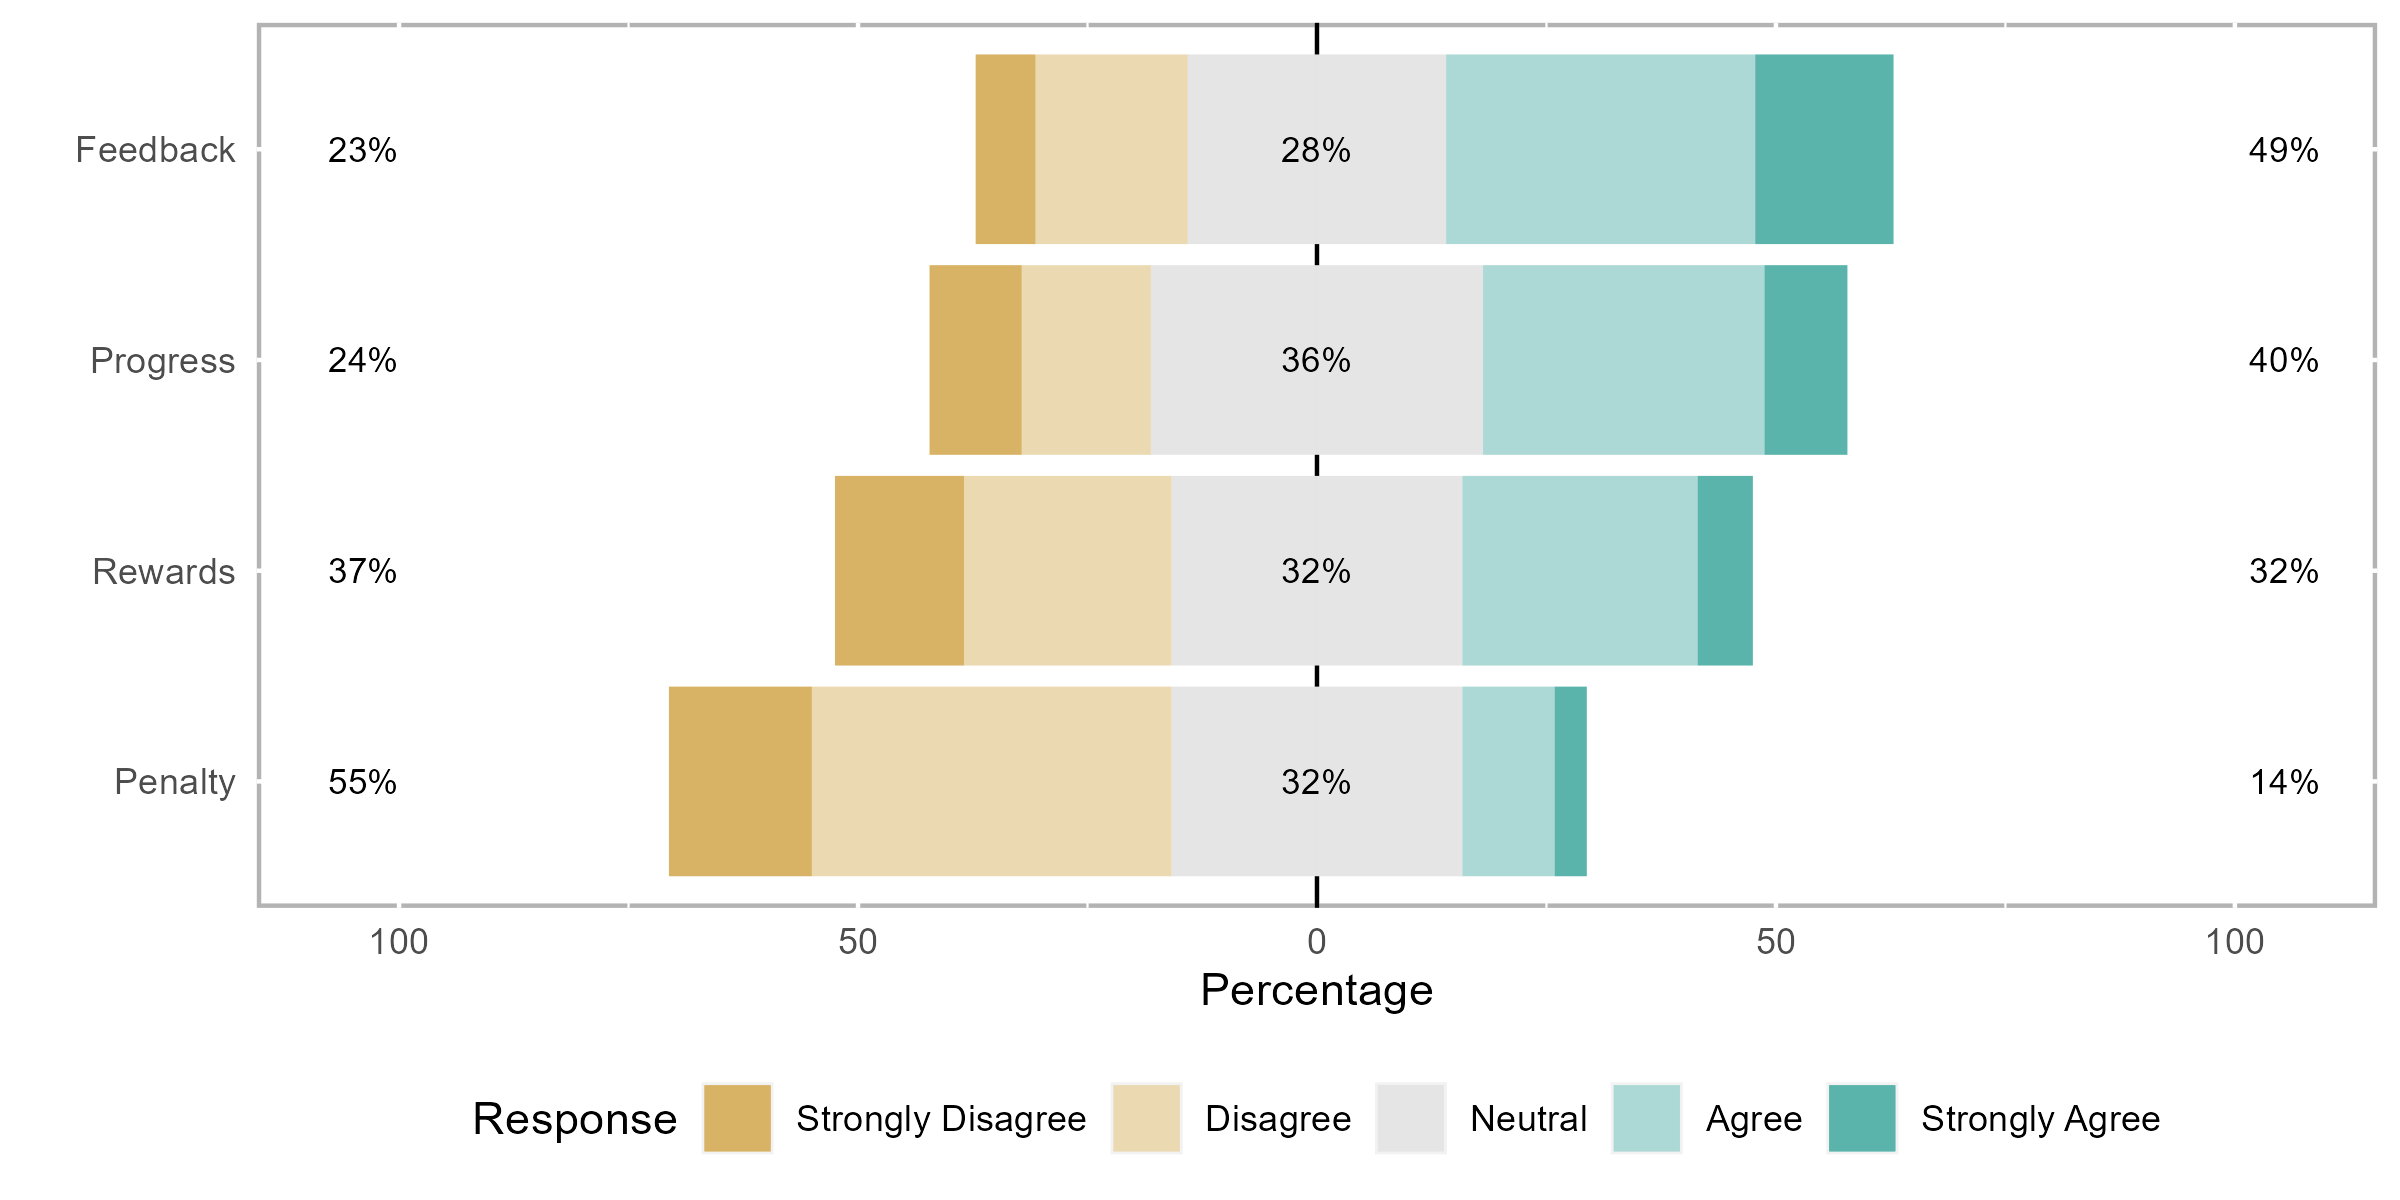
\includegraphics[width=\columnwidth]{Template_Latex_ScuDo_Tesi/Chapter3/exp_mechs.png}
\centering
\caption{Distribution of the average opinions related to the gamified mechanics' three constructs (influence, perceived usefulness, appreciation)}
\label{fig:m4overview}
\end{figure}

The most immediate result is a ranking of the four mechanics by student appreciation, with Feedback being the most appreciated, followed by Progress and Rewards, and Penalty being the least appreciated. It can be assumed that the students preferred mechanics that were helpful toward understanding the overall correctness of their diagrams by either pointing out which were the correct elements or by giving a sort of score, resulting in almost half the participants having a positive opinion of the Feedback mechanism, and 40\% of them appreciating the Progress indicator.

It is not surprising that the Penalty mechanic was the least appreciated, with 55\% of the students having a negative opinion about it, due to its implementation being tied to representing a reduction in the grade; a possible cause of concern, however, is the fact that penalties were reapplied after every check, and it was possible for students to reduce their grade very quickly, with no way to raise it back up, which may have increased even more the frustration aspect of penalization. Additionally, the grade could get reduced all the way down to 0, resulting in possible discomfort and loss of motivation; the Penalty mechanic, in combination with the single reference solution for each exercise, may have impacted negatively some students' opinion by making them believe their solution was incorrect and punishing them continuously.

Finally, and perhaps surprisingly when thinking back on the results of the preliminary assessment, the Rewards mechanic in the form of the jigsaw puzzle was ranked third among the mechanics, with a somewhat balanced distribution of opinions (32\% positive opinions, 32\% neutral, 36\% negative), making it less appreciated in comparison to how it was considered the best mechanic in the original test. A possible reason for this disapproval may come from the fact that the points needed to purchase pieces of the puzzle were tied to modeling the necessary parts in an acceptable way, and with a single solution not many students may have been able to do so.

Out of the 199 answers given to the open question related to the issues encountered during the experience, the open coding process revealed that 100 answers either mentioned no issue or had no explanation; a similar procedure was performed on the question asking for suggestion, where a total of 82 answers containing no comment were removed. The resulting topics obtained with the open coding analysis have been assigned to the various answers, and the counts of each tagged answer can be seen in Figure \ref{fig:issues_count} for the question about issues and in Figure \ref{fig:comments_count} for the one about improvement areas.


\begin{figure}[H]
    \centering
    \begin{subfigure}{0.6\linewidth}
        \centering
        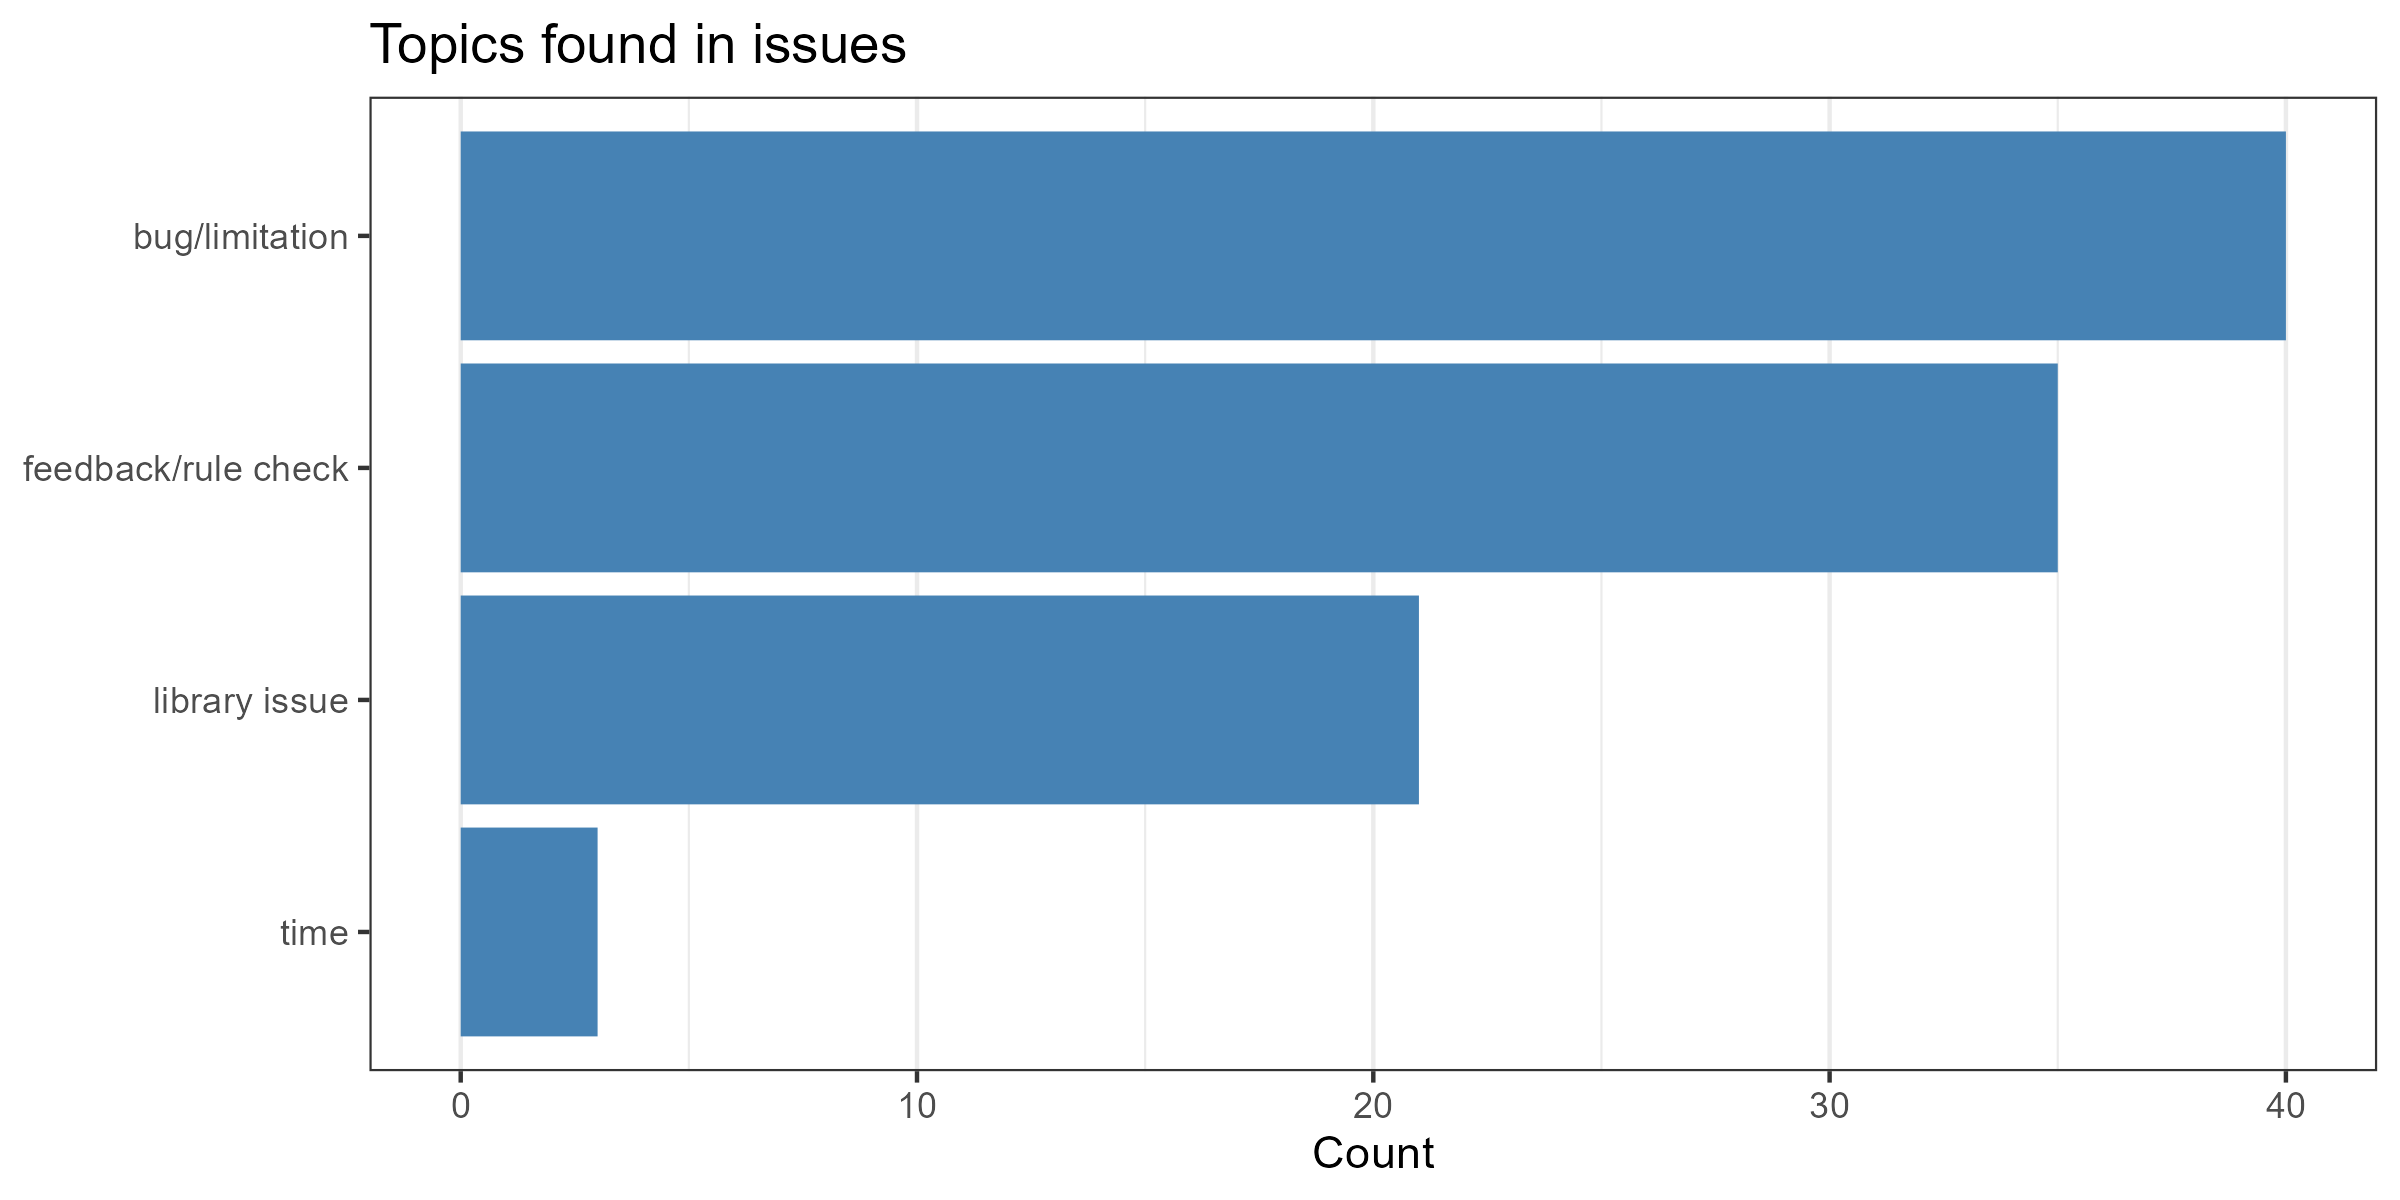
\includegraphics[width=\linewidth]{Template_Latex_ScuDo_Tesi/Chapter3/exp_issues.png}
        \caption{Topics found in the issues reported by the students}
        \label{fig:issues_count}
    \end{subfigure}\hfill
    \begin{subfigure}{0.6\linewidth}
        \centering
        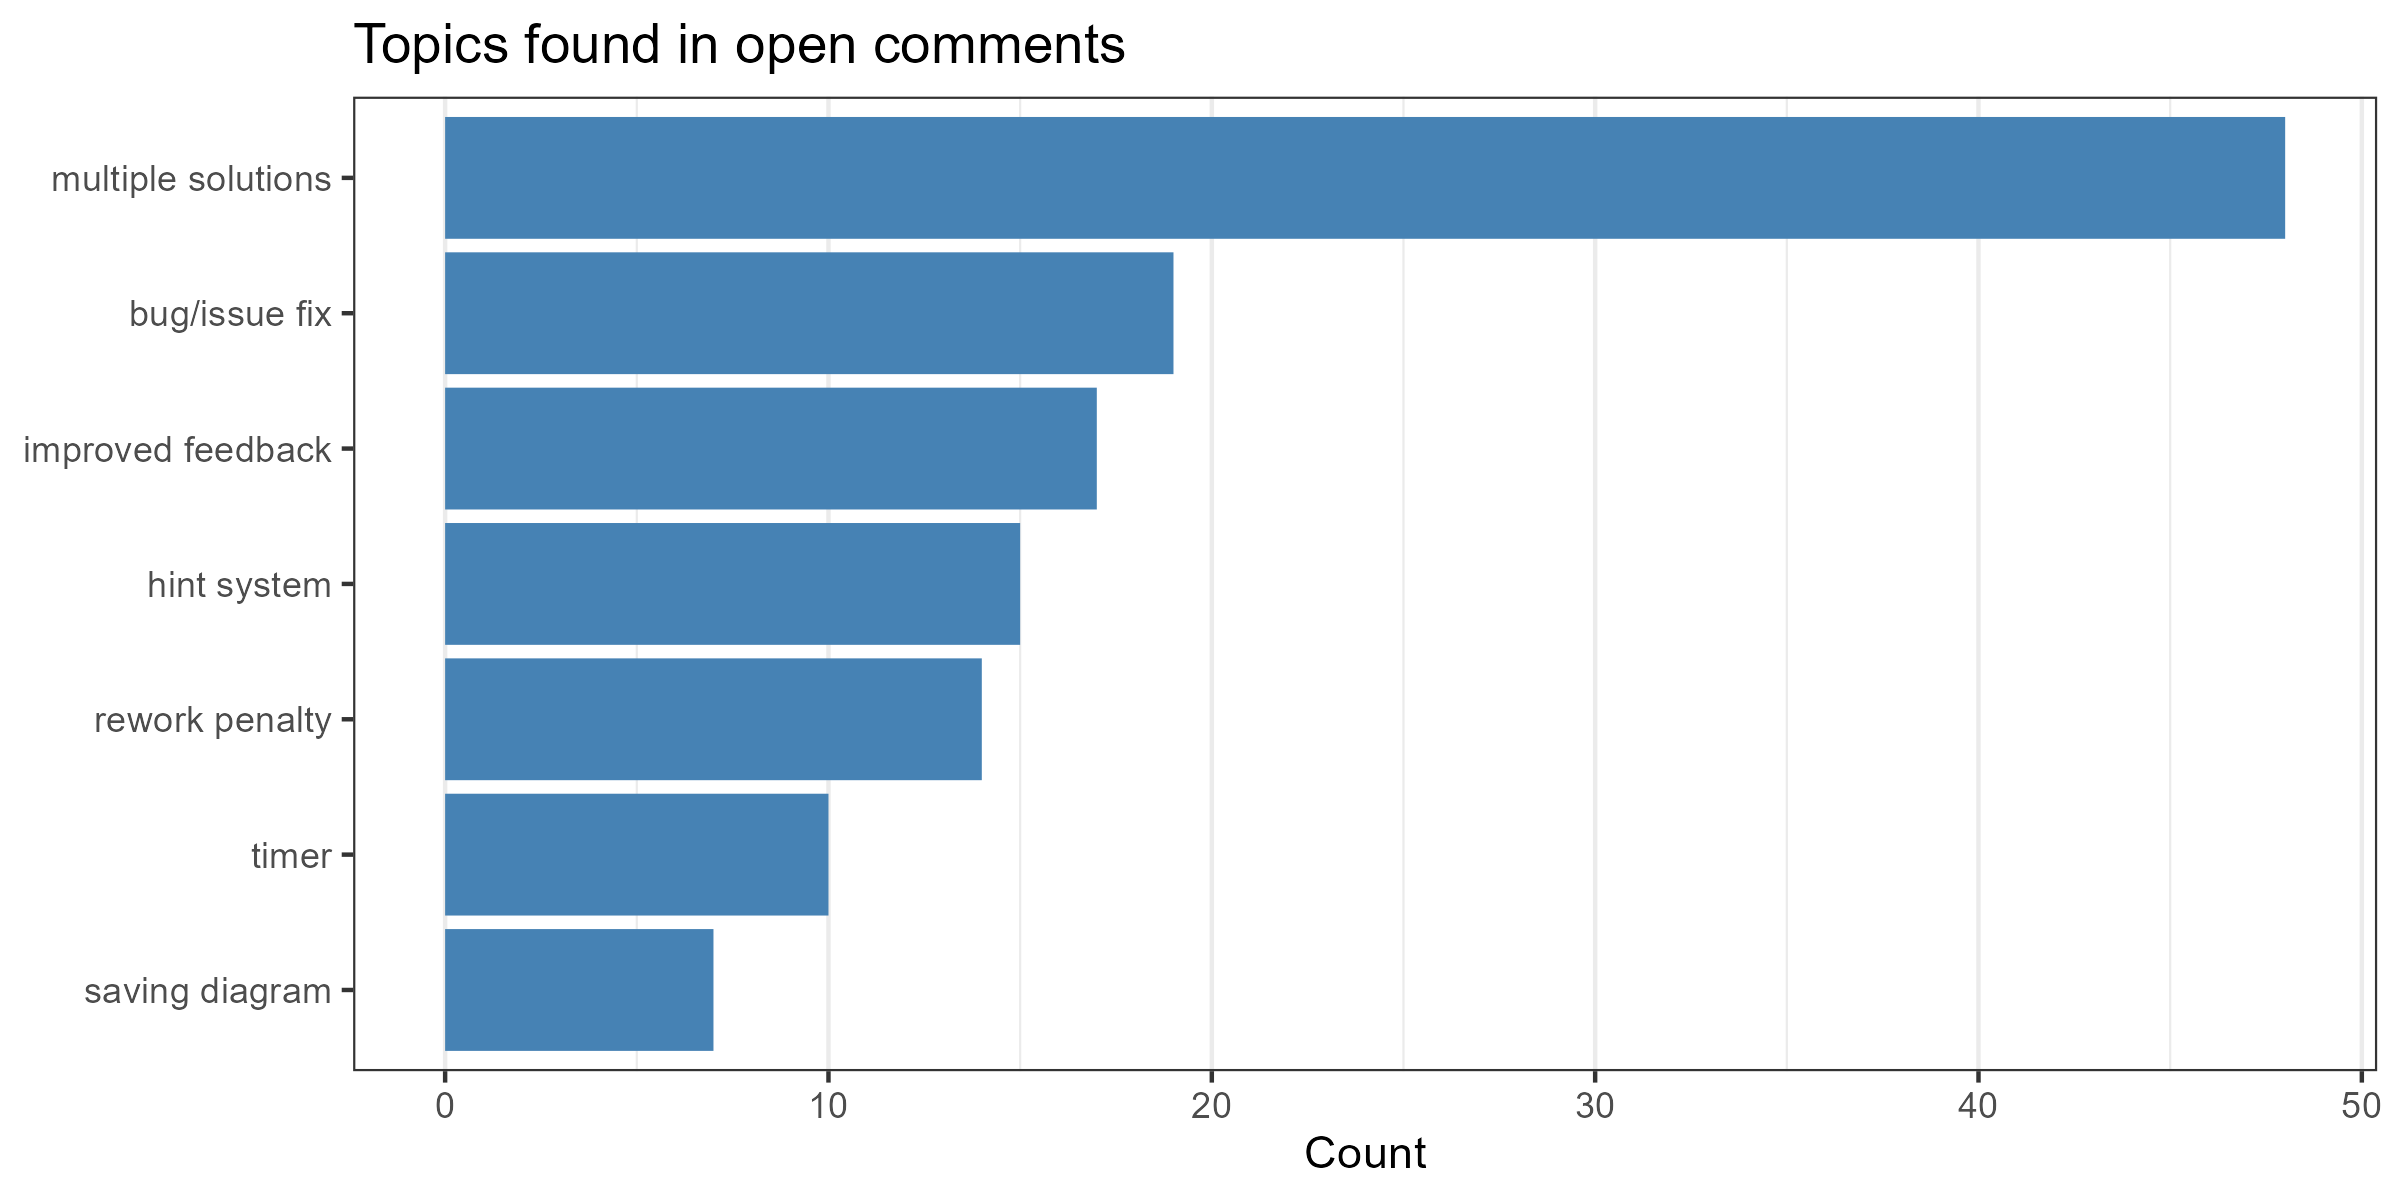
\includegraphics[width=\linewidth]{Template_Latex_ScuDo_Tesi/Chapter3/exp_comments.png}
        \caption{Topics found in the suggestions left by the students}
        \label{fig:comments_count}
    \end{subfigure}
    \caption{Results of the open coding procedure performed on the students' open answers}
    \label{fig:m4}
\end{figure}

The most common topic found among the issues relates to limitations of the way BIPMIN was implemented for the experiment such as the inability to save a BPMN diagram (the implemented version only saved data related to the game mechanics) or the problems that came from structuring the experiment as both in-person and online. Other issues were related to how the feedback mechanic was implemented and, as a consequence, with the way elements were checked for correctness matching; some issues were also caused by the libraries used to implement the BPMN modeling canvas, which showed some issues such as the inability to resize elements, or rare bugs where a drawn diagram would disappear out of view and become impossible to retrieve. Moreover, a very small issue was found in the time constraints of the experiment, with three students feeling the time allocated for each exercise was not sufficient for successful completion: time limits were enforced only due to the experimental nature, and real classroom use would not impose such constraints.

Topics found in the suggestions, instead, touch multiple details: the most common one is a request to support multiple solutions and, in general, allow more variety in the accepted ways to represent process parts, pointing to the single solution aspect being the most obvious limitation of BIPMIN. A second common topic focuses on addressing and fixing some of the bugs that had emerged, as well as the issues discussed in the preceding question, and several answers specifically suggested to add the ability for students to save their diagrams. Other suggestions focused on changing the game implementation such as adding a hint system, reworking the implementation of the Penalty mechanic to make it less strict, and expanding the feedback mechanism so that it would also give explanations on why certain elements were considered correct.

\answer{RQ4}{Students perceived favorably the gamified experience, and appreciated the most the game mechanics that were effective in guiding them toward drawing a correct BPMN model. On the other hand, mechanics that depended on producing a correct solution were less appreciated due to the strict evaluation engine that was limited to a single reference solution. The open questions reinforce this interpretation, as it was the most common suggestion and several issues derived from it.}


%After the questionnaire results were obtained, we performed an analysis of face validity and content validity of the various questions where each author expressed a rating for each question: for face validity, authors expressed whether each question was relevant or not, and for content validity authors had to choose whether questions were necessary, useful but not necessary, and not necessary. The analysis showed that questions Q2.3, Q2.4, Q5.2, and Q6.2 of the GAMEX questionnaire were unanimously considered to not be relevant and that questions Q2.3, Q2.4, and Q5.2 were unanimously judged to not be necessary; those questions were thus excluded when computing the distribution of answers to the GAMEX questionnaire. The content of each removed item can be seen in Appendix \ref{app:questionnaire} at the end of this paper. Sarà vero? E io che cazzo ne so


\subsubsection{Threats to validity}

Threats to validity are discussed following the taxonomy introduced in Section \ref{sec:empirical_methods} \cite{wohlin2012experimentation}.

\textbf{Threats to internal validity} relate mostly to the experimental design being a crossover study: the study was composed of two consecutive tasks, each with a given time limit, implying the possible presence of fatigue effects on the students. Additionally, executing two tasks in immediate sequence means that there could be possible carryover effects by administering a treatment before the effects of a different treatment have been completely received. The experiment design being a 2x2 factorial is helpful in mitigating learning biases; despite that, having students perform the tasks using two different versions of the same tool with one being enhanced means that there could be possible learning effects impacting the results of the second tasks, as a consequence of the students becoming familiar to the basic mechanics of the tool; the crossover design also implies that the second task's results may be impacted by learning and fatigue effects \cite{vegas2016crossover}.

Additionally, the two selected exercises pose another threat to the internal validity of the results, since it cannot be assumed that exercises of different difficulty would lead to comparable results. The two exercises were assumed to have a comparable level of difficulty, but the results showed that one was, in practice, slightly easier.

\textbf{Threats to external validity} concern the students who took part in the experiment, since the experiment could have different results if used by students with different skill levels (e.g., at the beginning of a course rather than toward the end) or by students of a different course with a different approach to teaching BPMN. Additionally, the results cannot be generalized to a non-educational context, meaning that BIPMIN may possibly not be effective if adopted in an industrial modeling scenario, for example.

\textbf{Threats to construct validity} for this study are connected to the metrics selected to answer RQ1 and RQ2, since other metrics may have been more suitable to represent the intended constructs.
\textit{Productivity} may have also been measured with the time spent for completing each exercise, since a maximum time of 45 minutes per exercise was defined as a study constraints, and students who were able to complete an exercise before said limit could be said to be more productive. However, since spending less time does not necessarily imply correctness, and students could possibly try to finish exercises quickly to end the study, and thus time was not measured for the analysis. 

For \textit{Correctness}, instead, the criteria that were selected for the analysis may not have been the most effective in actually measuring a diagram's correctness. The evaluator considered semantic correctness as the count of elements that satisfied predefined sets of requirements, but it could have also been measured by checking for the presence or absence of elements considered errors; additionally, the accepted elements with their modeling constraints do not cover all possible alternative representation of the same process part, for example, with the risk of some correct diagrams being considered incorrect.

\textbf{Threats to conclusion validity} derive from the statistical analysis and the experimental design. The metrics were recorded automatically by the tool, so it can be assumed that no human error impacted their collection for the analysis; additionally, the statistical analysis was performed with nonparametric statistical tests that have no prerequisites.

Furthermore, the participants were assigned randomly to one of the four groups, with no preceding assessment of the BPMN modeling expertise of the participants, meaning that the random allocation may have impacted the results of the analysis, and a different allocation may have led to different results. The high number of participants, and the fact that the study was conducted at the end of the course, when students could be assumed to have a reasonably similar BPMN modeling skill level, means that this threat can be considered improbable, although not completely dismissible.

\subsection{Key findings and lessons learned}

The empirical study performed with the improved version of BIPMIN aimed at investigating whether adding gamification elements to a BPMN modeling application could have potential benefits in terms of influencing students' performance and engagement with the discipline. The results were somewhat mixed, identifying some positive effects as well as potentially critical issues to address before deploying the application to a real classroom environment.

The first point of interest observed was the impact on student performance, measured by observing the size of the saved diagrams and the number of times students submitted their diagrams for grading to the automated evaluation engine: while size was not impacted in any way by the use of gamification, it emerged that students were more willing to perform evaluations when using the gamified version, as that version tied game mechanics to the results of the automated checks. It can be deduced that, while gamification does not cause significant changes in the students' modeling habits such as adding or removing multiple elements, it can be beneficial by guiding them toward checking more frequently whether their solutions are correct or not.

Furthermore, to measure the potential positive effects of BIPMIN, diagram correctness was measured as both syntactic and semantic. The former was not impacted by gamification, as scores were on average high among both the gamified tool and its non-gamified counterpart: this is due to the experiment being placed at the end of the course, with students having a sufficient level of knowledge to handle advanced BPMN modeling rules. Future uses of BIPMIN should focus on assessing whether it can also be effective to enhance syntax knowledge by adopting it over longer periods of time, or at the earlier parts of a course.

Semantic correctness, instead, benefited from the adoption of gamification, as it increased significantly compared to non-gamified modeling: this is undoubtedly the most important and encouraging result achieved with the experiment, as it proves that gamification of model education can be effective and, thus, should be explored more. The cause behind this positive result can probably be attributed to the implemented game mechanics and their interaction with the inner evaluation engine: by having a dedicated way to express feedback for successful modeling actions and by offering a way for students to gauge how close they are to successful completion, BIPMIN managed to enhance the way in which exercise-specific constraints were represented: furthermore, these mechanics were the most appreciated ones, implying that detailed correctness feedback and indicators were strong mechanics on which further development would have to focus on.

However, the overall perception of the experiment was not completely positive due to inherent issues in the implementation: first of all, while the evaluation engine had been improved to allow for semantic checks on the content of the diagrams under evaluation, and measures for variety in the allowed solutions had been added, the reference solution was still a single one, with almost no variability included in the possible process parts. This resulted in several scenarios where students had produced a diagram that was, to the human eye, equivalent to the expected one but that was not considered correct by the automated evaluator; in turn, this meant continuous penalization and difficulty in obtaining points, resulting in two game mechanics (Rewards, Penalty) not being appreciated as much as the other two.

The post-experiment questionnaire also highlighted the issue in the implementation: not only most of the issues and suggestions were related to the evaluation engine and its limits, but answers to the GAMEX questionnaire were on the more neutral side, presenting BIPMIN as a tool that is somewhat fun and engaging, but is not immersive and does not allow complete freedom of action and creativity. An encouraging point that emerged from the GAMEX answers, at least, is the fact that it is not perceived as a frustrating and antagonizing experience, meaning that there could be potential benefits by adopting it after improvements.

\articleSummary{
color1
}{
Summary of the BIPMIN empirical study
}{
The empirical study on BIPMIN showed that gamification can have some positive effects on the students' modeling habits, by encouraging them to evaluate their diagrams more and increasing the semantic correctness of their diagrams. However, the experience was not completely well received due to the strictness of the automated evaluator, as well as the implementation of some mechanics that could have been improved.
}

\begin{comment}

Regarding student enjoyment and perceived usefulness, answers to the questionnaire showed that students appreciated the feedback and progress mechanics present in the tool, while the same cannot be said for the rewarding aspect and the penalization, which were widely disliked. This distribution of answers, as well as the topics found in the answers to the open-ended questions, indicates that the combination of a penalty mechanism with a strict evaluation engine that only accepts a limited set of correct solutions is a severe limitation of the tool, as it makes using the tool frustrating and unfun. Keeping in mind the comments left by students, we can see that the penalty system can be improved with the addition of a hint system or a variation that penalizes only serious mistakes; the implementation of this mechanic is still in its early stages, so there is room for improvement. Another possible solution would be to remove the mechanic entirely. 


\end{comment}